
% Default to the notebook output style

    


% Inherit from the specified cell style.




    
\documentclass[11pt]{article}

    
    
    \usepackage[T1]{fontenc}
    % Nicer default font (+ math font) than Computer Modern for most use cases
    \usepackage{mathpazo}

    % Basic figure setup, for now with no caption control since it's done
    % automatically by Pandoc (which extracts ![](path) syntax from Markdown).
    \usepackage{graphicx}
    % We will generate all images so they have a width \maxwidth. This means
    % that they will get their normal width if they fit onto the page, but
    % are scaled down if they would overflow the margins.
    \makeatletter
    \def\maxwidth{\ifdim\Gin@nat@width>\linewidth\linewidth
    \else\Gin@nat@width\fi}
    \makeatother
    \let\Oldincludegraphics\includegraphics
    % Set max figure width to be 80% of text width, for now hardcoded.
    \renewcommand{\includegraphics}[1]{\Oldincludegraphics[width=.8\maxwidth]{#1}}
    % Ensure that by default, figures have no caption (until we provide a
    % proper Figure object with a Caption API and a way to capture that
    % in the conversion process - todo).
    \usepackage{caption}
    \DeclareCaptionLabelFormat{nolabel}{}
    \captionsetup{labelformat=nolabel}

    \usepackage{adjustbox} % Used to constrain images to a maximum size 
    \usepackage{xcolor} % Allow colors to be defined
    \usepackage{enumerate} % Needed for markdown enumerations to work
    \usepackage{geometry} % Used to adjust the document margins
    \usepackage{amsmath} % Equations
    \usepackage{amssymb} % Equations
    \usepackage{textcomp} % defines textquotesingle
    % Hack from http://tex.stackexchange.com/a/47451/13684:
    \AtBeginDocument{%
        \def\PYZsq{\textquotesingle}% Upright quotes in Pygmentized code
    }
    \usepackage{upquote} % Upright quotes for verbatim code
    \usepackage{eurosym} % defines \euro
    \usepackage[mathletters]{ucs} % Extended unicode (utf-8) support
    \usepackage[utf8x]{inputenc} % Allow utf-8 characters in the tex document
    \usepackage{fancyvrb} % verbatim replacement that allows latex
    \usepackage{grffile} % extends the file name processing of package graphics 
                         % to support a larger range 
    % The hyperref package gives us a pdf with properly built
    % internal navigation ('pdf bookmarks' for the table of contents,
    % internal cross-reference links, web links for URLs, etc.)
    \usepackage{hyperref}
    \usepackage{longtable} % longtable support required by pandoc >1.10
    \usepackage{booktabs}  % table support for pandoc > 1.12.2
    \usepackage[inline]{enumitem} % IRkernel/repr support (it uses the enumerate* environment)
    \usepackage[normalem]{ulem} % ulem is needed to support strikethroughs (\sout)
                                % normalem makes italics be italics, not underlines
    

    
    
    % Colors for the hyperref package
    \definecolor{urlcolor}{rgb}{0,.145,.698}
    \definecolor{linkcolor}{rgb}{.71,0.21,0.01}
    \definecolor{citecolor}{rgb}{.12,.54,.11}

    % ANSI colors
    \definecolor{ansi-black}{HTML}{3E424D}
    \definecolor{ansi-black-intense}{HTML}{282C36}
    \definecolor{ansi-red}{HTML}{E75C58}
    \definecolor{ansi-red-intense}{HTML}{B22B31}
    \definecolor{ansi-green}{HTML}{00A250}
    \definecolor{ansi-green-intense}{HTML}{007427}
    \definecolor{ansi-yellow}{HTML}{DDB62B}
    \definecolor{ansi-yellow-intense}{HTML}{B27D12}
    \definecolor{ansi-blue}{HTML}{208FFB}
    \definecolor{ansi-blue-intense}{HTML}{0065CA}
    \definecolor{ansi-magenta}{HTML}{D160C4}
    \definecolor{ansi-magenta-intense}{HTML}{A03196}
    \definecolor{ansi-cyan}{HTML}{60C6C8}
    \definecolor{ansi-cyan-intense}{HTML}{258F8F}
    \definecolor{ansi-white}{HTML}{C5C1B4}
    \definecolor{ansi-white-intense}{HTML}{A1A6B2}

    % commands and environments needed by pandoc snippets
    % extracted from the output of `pandoc -s`
    \providecommand{\tightlist}{%
      \setlength{\itemsep}{0pt}\setlength{\parskip}{0pt}}
    \DefineVerbatimEnvironment{Highlighting}{Verbatim}{commandchars=\\\{\}}
    % Add ',fontsize=\small' for more characters per line
    \newenvironment{Shaded}{}{}
    \newcommand{\KeywordTok}[1]{\textcolor[rgb]{0.00,0.44,0.13}{\textbf{{#1}}}}
    \newcommand{\DataTypeTok}[1]{\textcolor[rgb]{0.56,0.13,0.00}{{#1}}}
    \newcommand{\DecValTok}[1]{\textcolor[rgb]{0.25,0.63,0.44}{{#1}}}
    \newcommand{\BaseNTok}[1]{\textcolor[rgb]{0.25,0.63,0.44}{{#1}}}
    \newcommand{\FloatTok}[1]{\textcolor[rgb]{0.25,0.63,0.44}{{#1}}}
    \newcommand{\CharTok}[1]{\textcolor[rgb]{0.25,0.44,0.63}{{#1}}}
    \newcommand{\StringTok}[1]{\textcolor[rgb]{0.25,0.44,0.63}{{#1}}}
    \newcommand{\CommentTok}[1]{\textcolor[rgb]{0.38,0.63,0.69}{\textit{{#1}}}}
    \newcommand{\OtherTok}[1]{\textcolor[rgb]{0.00,0.44,0.13}{{#1}}}
    \newcommand{\AlertTok}[1]{\textcolor[rgb]{1.00,0.00,0.00}{\textbf{{#1}}}}
    \newcommand{\FunctionTok}[1]{\textcolor[rgb]{0.02,0.16,0.49}{{#1}}}
    \newcommand{\RegionMarkerTok}[1]{{#1}}
    \newcommand{\ErrorTok}[1]{\textcolor[rgb]{1.00,0.00,0.00}{\textbf{{#1}}}}
    \newcommand{\NormalTok}[1]{{#1}}
    
    % Additional commands for more recent versions of Pandoc
    \newcommand{\ConstantTok}[1]{\textcolor[rgb]{0.53,0.00,0.00}{{#1}}}
    \newcommand{\SpecialCharTok}[1]{\textcolor[rgb]{0.25,0.44,0.63}{{#1}}}
    \newcommand{\VerbatimStringTok}[1]{\textcolor[rgb]{0.25,0.44,0.63}{{#1}}}
    \newcommand{\SpecialStringTok}[1]{\textcolor[rgb]{0.73,0.40,0.53}{{#1}}}
    \newcommand{\ImportTok}[1]{{#1}}
    \newcommand{\DocumentationTok}[1]{\textcolor[rgb]{0.73,0.13,0.13}{\textit{{#1}}}}
    \newcommand{\AnnotationTok}[1]{\textcolor[rgb]{0.38,0.63,0.69}{\textbf{\textit{{#1}}}}}
    \newcommand{\CommentVarTok}[1]{\textcolor[rgb]{0.38,0.63,0.69}{\textbf{\textit{{#1}}}}}
    \newcommand{\VariableTok}[1]{\textcolor[rgb]{0.10,0.09,0.49}{{#1}}}
    \newcommand{\ControlFlowTok}[1]{\textcolor[rgb]{0.00,0.44,0.13}{\textbf{{#1}}}}
    \newcommand{\OperatorTok}[1]{\textcolor[rgb]{0.40,0.40,0.40}{{#1}}}
    \newcommand{\BuiltInTok}[1]{{#1}}
    \newcommand{\ExtensionTok}[1]{{#1}}
    \newcommand{\PreprocessorTok}[1]{\textcolor[rgb]{0.74,0.48,0.00}{{#1}}}
    \newcommand{\AttributeTok}[1]{\textcolor[rgb]{0.49,0.56,0.16}{{#1}}}
    \newcommand{\InformationTok}[1]{\textcolor[rgb]{0.38,0.63,0.69}{\textbf{\textit{{#1}}}}}
    \newcommand{\WarningTok}[1]{\textcolor[rgb]{0.38,0.63,0.69}{\textbf{\textit{{#1}}}}}
    
    
    % Define a nice break command that doesn't care if a line doesn't already
    % exist.
    \def\br{\hspace*{\fill} \\* }
    % Math Jax compatability definitions
    \def\gt{>}
    \def\lt{<}
    % Document parameters
    \title{Deep Learning ??? MLP ver.2.1}
    
    
    

    % Pygments definitions
    
\makeatletter
\def\PY@reset{\let\PY@it=\relax \let\PY@bf=\relax%
    \let\PY@ul=\relax \let\PY@tc=\relax%
    \let\PY@bc=\relax \let\PY@ff=\relax}
\def\PY@tok#1{\csname PY@tok@#1\endcsname}
\def\PY@toks#1+{\ifx\relax#1\empty\else%
    \PY@tok{#1}\expandafter\PY@toks\fi}
\def\PY@do#1{\PY@bc{\PY@tc{\PY@ul{%
    \PY@it{\PY@bf{\PY@ff{#1}}}}}}}
\def\PY#1#2{\PY@reset\PY@toks#1+\relax+\PY@do{#2}}

\expandafter\def\csname PY@tok@w\endcsname{\def\PY@tc##1{\textcolor[rgb]{0.73,0.73,0.73}{##1}}}
\expandafter\def\csname PY@tok@c\endcsname{\let\PY@it=\textit\def\PY@tc##1{\textcolor[rgb]{0.25,0.50,0.50}{##1}}}
\expandafter\def\csname PY@tok@cp\endcsname{\def\PY@tc##1{\textcolor[rgb]{0.74,0.48,0.00}{##1}}}
\expandafter\def\csname PY@tok@k\endcsname{\let\PY@bf=\textbf\def\PY@tc##1{\textcolor[rgb]{0.00,0.50,0.00}{##1}}}
\expandafter\def\csname PY@tok@kp\endcsname{\def\PY@tc##1{\textcolor[rgb]{0.00,0.50,0.00}{##1}}}
\expandafter\def\csname PY@tok@kt\endcsname{\def\PY@tc##1{\textcolor[rgb]{0.69,0.00,0.25}{##1}}}
\expandafter\def\csname PY@tok@o\endcsname{\def\PY@tc##1{\textcolor[rgb]{0.40,0.40,0.40}{##1}}}
\expandafter\def\csname PY@tok@ow\endcsname{\let\PY@bf=\textbf\def\PY@tc##1{\textcolor[rgb]{0.67,0.13,1.00}{##1}}}
\expandafter\def\csname PY@tok@nb\endcsname{\def\PY@tc##1{\textcolor[rgb]{0.00,0.50,0.00}{##1}}}
\expandafter\def\csname PY@tok@nf\endcsname{\def\PY@tc##1{\textcolor[rgb]{0.00,0.00,1.00}{##1}}}
\expandafter\def\csname PY@tok@nc\endcsname{\let\PY@bf=\textbf\def\PY@tc##1{\textcolor[rgb]{0.00,0.00,1.00}{##1}}}
\expandafter\def\csname PY@tok@nn\endcsname{\let\PY@bf=\textbf\def\PY@tc##1{\textcolor[rgb]{0.00,0.00,1.00}{##1}}}
\expandafter\def\csname PY@tok@ne\endcsname{\let\PY@bf=\textbf\def\PY@tc##1{\textcolor[rgb]{0.82,0.25,0.23}{##1}}}
\expandafter\def\csname PY@tok@nv\endcsname{\def\PY@tc##1{\textcolor[rgb]{0.10,0.09,0.49}{##1}}}
\expandafter\def\csname PY@tok@no\endcsname{\def\PY@tc##1{\textcolor[rgb]{0.53,0.00,0.00}{##1}}}
\expandafter\def\csname PY@tok@nl\endcsname{\def\PY@tc##1{\textcolor[rgb]{0.63,0.63,0.00}{##1}}}
\expandafter\def\csname PY@tok@ni\endcsname{\let\PY@bf=\textbf\def\PY@tc##1{\textcolor[rgb]{0.60,0.60,0.60}{##1}}}
\expandafter\def\csname PY@tok@na\endcsname{\def\PY@tc##1{\textcolor[rgb]{0.49,0.56,0.16}{##1}}}
\expandafter\def\csname PY@tok@nt\endcsname{\let\PY@bf=\textbf\def\PY@tc##1{\textcolor[rgb]{0.00,0.50,0.00}{##1}}}
\expandafter\def\csname PY@tok@nd\endcsname{\def\PY@tc##1{\textcolor[rgb]{0.67,0.13,1.00}{##1}}}
\expandafter\def\csname PY@tok@s\endcsname{\def\PY@tc##1{\textcolor[rgb]{0.73,0.13,0.13}{##1}}}
\expandafter\def\csname PY@tok@sd\endcsname{\let\PY@it=\textit\def\PY@tc##1{\textcolor[rgb]{0.73,0.13,0.13}{##1}}}
\expandafter\def\csname PY@tok@si\endcsname{\let\PY@bf=\textbf\def\PY@tc##1{\textcolor[rgb]{0.73,0.40,0.53}{##1}}}
\expandafter\def\csname PY@tok@se\endcsname{\let\PY@bf=\textbf\def\PY@tc##1{\textcolor[rgb]{0.73,0.40,0.13}{##1}}}
\expandafter\def\csname PY@tok@sr\endcsname{\def\PY@tc##1{\textcolor[rgb]{0.73,0.40,0.53}{##1}}}
\expandafter\def\csname PY@tok@ss\endcsname{\def\PY@tc##1{\textcolor[rgb]{0.10,0.09,0.49}{##1}}}
\expandafter\def\csname PY@tok@sx\endcsname{\def\PY@tc##1{\textcolor[rgb]{0.00,0.50,0.00}{##1}}}
\expandafter\def\csname PY@tok@m\endcsname{\def\PY@tc##1{\textcolor[rgb]{0.40,0.40,0.40}{##1}}}
\expandafter\def\csname PY@tok@gh\endcsname{\let\PY@bf=\textbf\def\PY@tc##1{\textcolor[rgb]{0.00,0.00,0.50}{##1}}}
\expandafter\def\csname PY@tok@gu\endcsname{\let\PY@bf=\textbf\def\PY@tc##1{\textcolor[rgb]{0.50,0.00,0.50}{##1}}}
\expandafter\def\csname PY@tok@gd\endcsname{\def\PY@tc##1{\textcolor[rgb]{0.63,0.00,0.00}{##1}}}
\expandafter\def\csname PY@tok@gi\endcsname{\def\PY@tc##1{\textcolor[rgb]{0.00,0.63,0.00}{##1}}}
\expandafter\def\csname PY@tok@gr\endcsname{\def\PY@tc##1{\textcolor[rgb]{1.00,0.00,0.00}{##1}}}
\expandafter\def\csname PY@tok@ge\endcsname{\let\PY@it=\textit}
\expandafter\def\csname PY@tok@gs\endcsname{\let\PY@bf=\textbf}
\expandafter\def\csname PY@tok@gp\endcsname{\let\PY@bf=\textbf\def\PY@tc##1{\textcolor[rgb]{0.00,0.00,0.50}{##1}}}
\expandafter\def\csname PY@tok@go\endcsname{\def\PY@tc##1{\textcolor[rgb]{0.53,0.53,0.53}{##1}}}
\expandafter\def\csname PY@tok@gt\endcsname{\def\PY@tc##1{\textcolor[rgb]{0.00,0.27,0.87}{##1}}}
\expandafter\def\csname PY@tok@err\endcsname{\def\PY@bc##1{\setlength{\fboxsep}{0pt}\fcolorbox[rgb]{1.00,0.00,0.00}{1,1,1}{\strut ##1}}}
\expandafter\def\csname PY@tok@kc\endcsname{\let\PY@bf=\textbf\def\PY@tc##1{\textcolor[rgb]{0.00,0.50,0.00}{##1}}}
\expandafter\def\csname PY@tok@kd\endcsname{\let\PY@bf=\textbf\def\PY@tc##1{\textcolor[rgb]{0.00,0.50,0.00}{##1}}}
\expandafter\def\csname PY@tok@kn\endcsname{\let\PY@bf=\textbf\def\PY@tc##1{\textcolor[rgb]{0.00,0.50,0.00}{##1}}}
\expandafter\def\csname PY@tok@kr\endcsname{\let\PY@bf=\textbf\def\PY@tc##1{\textcolor[rgb]{0.00,0.50,0.00}{##1}}}
\expandafter\def\csname PY@tok@bp\endcsname{\def\PY@tc##1{\textcolor[rgb]{0.00,0.50,0.00}{##1}}}
\expandafter\def\csname PY@tok@fm\endcsname{\def\PY@tc##1{\textcolor[rgb]{0.00,0.00,1.00}{##1}}}
\expandafter\def\csname PY@tok@vc\endcsname{\def\PY@tc##1{\textcolor[rgb]{0.10,0.09,0.49}{##1}}}
\expandafter\def\csname PY@tok@vg\endcsname{\def\PY@tc##1{\textcolor[rgb]{0.10,0.09,0.49}{##1}}}
\expandafter\def\csname PY@tok@vi\endcsname{\def\PY@tc##1{\textcolor[rgb]{0.10,0.09,0.49}{##1}}}
\expandafter\def\csname PY@tok@vm\endcsname{\def\PY@tc##1{\textcolor[rgb]{0.10,0.09,0.49}{##1}}}
\expandafter\def\csname PY@tok@sa\endcsname{\def\PY@tc##1{\textcolor[rgb]{0.73,0.13,0.13}{##1}}}
\expandafter\def\csname PY@tok@sb\endcsname{\def\PY@tc##1{\textcolor[rgb]{0.73,0.13,0.13}{##1}}}
\expandafter\def\csname PY@tok@sc\endcsname{\def\PY@tc##1{\textcolor[rgb]{0.73,0.13,0.13}{##1}}}
\expandafter\def\csname PY@tok@dl\endcsname{\def\PY@tc##1{\textcolor[rgb]{0.73,0.13,0.13}{##1}}}
\expandafter\def\csname PY@tok@s2\endcsname{\def\PY@tc##1{\textcolor[rgb]{0.73,0.13,0.13}{##1}}}
\expandafter\def\csname PY@tok@sh\endcsname{\def\PY@tc##1{\textcolor[rgb]{0.73,0.13,0.13}{##1}}}
\expandafter\def\csname PY@tok@s1\endcsname{\def\PY@tc##1{\textcolor[rgb]{0.73,0.13,0.13}{##1}}}
\expandafter\def\csname PY@tok@mb\endcsname{\def\PY@tc##1{\textcolor[rgb]{0.40,0.40,0.40}{##1}}}
\expandafter\def\csname PY@tok@mf\endcsname{\def\PY@tc##1{\textcolor[rgb]{0.40,0.40,0.40}{##1}}}
\expandafter\def\csname PY@tok@mh\endcsname{\def\PY@tc##1{\textcolor[rgb]{0.40,0.40,0.40}{##1}}}
\expandafter\def\csname PY@tok@mi\endcsname{\def\PY@tc##1{\textcolor[rgb]{0.40,0.40,0.40}{##1}}}
\expandafter\def\csname PY@tok@il\endcsname{\def\PY@tc##1{\textcolor[rgb]{0.40,0.40,0.40}{##1}}}
\expandafter\def\csname PY@tok@mo\endcsname{\def\PY@tc##1{\textcolor[rgb]{0.40,0.40,0.40}{##1}}}
\expandafter\def\csname PY@tok@ch\endcsname{\let\PY@it=\textit\def\PY@tc##1{\textcolor[rgb]{0.25,0.50,0.50}{##1}}}
\expandafter\def\csname PY@tok@cm\endcsname{\let\PY@it=\textit\def\PY@tc##1{\textcolor[rgb]{0.25,0.50,0.50}{##1}}}
\expandafter\def\csname PY@tok@cpf\endcsname{\let\PY@it=\textit\def\PY@tc##1{\textcolor[rgb]{0.25,0.50,0.50}{##1}}}
\expandafter\def\csname PY@tok@c1\endcsname{\let\PY@it=\textit\def\PY@tc##1{\textcolor[rgb]{0.25,0.50,0.50}{##1}}}
\expandafter\def\csname PY@tok@cs\endcsname{\let\PY@it=\textit\def\PY@tc##1{\textcolor[rgb]{0.25,0.50,0.50}{##1}}}

\def\PYZbs{\char`\\}
\def\PYZus{\char`\_}
\def\PYZob{\char`\{}
\def\PYZcb{\char`\}}
\def\PYZca{\char`\^}
\def\PYZam{\char`\&}
\def\PYZlt{\char`\<}
\def\PYZgt{\char`\>}
\def\PYZsh{\char`\#}
\def\PYZpc{\char`\%}
\def\PYZdl{\char`\$}
\def\PYZhy{\char`\-}
\def\PYZsq{\char`\'}
\def\PYZdq{\char`\"}
\def\PYZti{\char`\~}
% for compatibility with earlier versions
\def\PYZat{@}
\def\PYZlb{[}
\def\PYZrb{]}
\makeatother


    % Exact colors from NB
    \definecolor{incolor}{rgb}{0.0, 0.0, 0.5}
    \definecolor{outcolor}{rgb}{0.545, 0.0, 0.0}



    
    % Prevent overflowing lines due to hard-to-break entities
    \sloppy 
    % Setup hyperref package
    \hypersetup{
      breaklinks=true,  % so long urls are correctly broken across lines
      colorlinks=true,
      urlcolor=urlcolor,
      linkcolor=linkcolor,
      citecolor=citecolor,
      }
    % Slightly bigger margins than the latex defaults
    
    \geometry{verbose,tmargin=1in,bmargin=1in,lmargin=1in,rmargin=1in}
    
    

    \begin{document}
    
    
    \maketitle
    
    

    
    \hypertarget{analysis-uxacfcuxc815---deep-learning}{%
\section{Analysis 과정 - Deep
Learning}\label{analysis-uxacfcuxc815---deep-learning}}

    \hypertarget{uxac15uxc758-uxac1cuxc694}{%
\subsection{강의 개요}\label{uxac15uxc758-uxac1cuxc694}}

\begin{itemize}
\tightlist
\item
  왜 딥러닝인가?

  \begin{itemize}
  \tightlist
  \item
    통계, 머신러닝, 딥러닝의 차이
  \item
    딥러닝으로 풀 수 있는 문제
  \end{itemize}
\item
  딥러닝의 원리

  \begin{itemize}
  \tightlist
  \item
    학습이란?
  \item
    어떻게 데이터를 학습하는가
  \end{itemize}
\item
  딥러닝의 구조

  \begin{itemize}
  \tightlist
  \item
    입력 \(\rightarrow\) 모델 \(\rightarrow\) 출력
  \item
    Layer : 모델의 구성단위
  \item
    Activation : 비선형 모델로 가는 길
  \item
    Bias : 영점조절
  \end{itemize}
\item
  학습으로 돌아와서

  \begin{itemize}
  \tightlist
  \item
    Train Set : 기출 문제은행
  \item
    Batch : 모의고사
  \item
    Epoch : 1회독
  \item
    Step : 모의고사 응시횟수
  \item
    Loss : 시험점수
  \item
    Gradient : 공부방향
  \item
    Optimization : 공부방법
  \item
    Backpropagation : 오답노트, 복습
  \end{itemize}
\item
  모델 평가

  \begin{itemize}
  \tightlist
  \item
    Accuracy : 문제은행
  \item
    Batch : 모의고사
  \item
    Epoch : 1회독
  \item
    Step : 모의고사 응시횟수
  \end{itemize}
\item
  딥러닝의 발전

  \begin{itemize}
  \tightlist
  \item
    MLP : 다 엮어보자! 죄다 연결된 신경망 (Fully Connected), 빡빡한
    신경망 (Dense)
  \item
    CNN : Image를 부분으로 쪼개서 조금씩 보자!
  \item
    RNN : Data 순서에 의미가 있다면? 과거를 기억하자

    \begin{itemize}
    \tightlist
    \item
      Advanced RNN : 기억력 향상
    \end{itemize}
  \end{itemize}
\end{itemize}

    \hypertarget{uxac15uxc758-uxc9c4uxd589-uxacfcuxc815}{%
\subsubsection{강의 진행
과정}\label{uxac15uxc758-uxc9c4uxd589-uxacfcuxc815}}

\begin{itemize}
\tightlist
\item
  기본

  \begin{enumerate}
  \def\labelenumi{\arabic{enumi}.}
  \tightlist
  \item
    실습 진행 ( Code Review \& 작성 )
  \end{enumerate}

  \begin{itemize}
  \tightlist
  \item
    \texttt{keras}
  \end{itemize}

  \begin{enumerate}
  \def\labelenumi{\arabic{enumi}.}
  \setcounter{enumi}{1}
  \tightlist
  \item
    개념 설명
  \item
    개념 이해 ( Code Review )
  \end{enumerate}

  \begin{itemize}
  \tightlist
  \item
    \texttt{numpy}
  \end{itemize}
\item
  심화

  \begin{enumerate}
  \def\labelenumi{\arabic{enumi}.}
  \tightlist
  \item
    개념 반복
  \item
    실습 진행
  \end{enumerate}

  \begin{itemize}
  \tightlist
  \item
    \texttt{tensorflow}
  \end{itemize}
\end{itemize}

    \begin{center}\rule{0.5\linewidth}{\linethickness}\end{center}

\hypertarget{uxb525uxb7ecuxb2dd-uxac1cuxc694}{%
\subsection{딥러닝 개요}\label{uxb525uxb7ecuxb2dd-uxac1cuxc694}}

    \hypertarget{uxc65c-uxb525uxb7ecuxb2dduxc778uxac00}{%
\subsubsection{왜
딥러닝인가?}\label{uxc65c-uxb525uxb7ecuxb2dduxc778uxac00}}

``기계학습, 사람이 판단하기 힘든 규칙들을 데이터 양으로 극복해 보자!''

\begin{itemize}
\tightlist
\item
  M/L 기반 방법론

  \begin{itemize}
  \tightlist
  \item
    원리: 선형근사와 정규분포 가정을 기반으로 데이터를 잘 설명하는
    선형방정식을 만들어 새로운 Input에 대응하는 결과를 예측.
  \item
    학습: OLS, GLS 등 최소제곱합 또는 최대가능도추정, 분산감소기법 등의
    다소 학습이 빠른 기법들이 사용.
  \item
    목적: 변수를 최대한 활용하여 다소 복잡하고 설명력이 떨어지더라도
    좋은 예측력을 갖는 모델을 지향하며, 경우에 따라 주요 원인변수 선별도
    가능.
  \item
    평가: 오차의 크기, 정확도(Accuracy) 및 Precision/Recall 등
    예측결과에 대한 지표들이 주로 사용. 
  \end{itemize}
\end{itemize}

\begin{center}\rule{0.5\linewidth}{\linethickness}\end{center}

\begin{itemize}
\tightlist
\item
  D/L 기반 방법론

  \begin{itemize}
  \tightlist
  \item
    원리: 비선형모델을 기반으로 데이터를 잘 설명하는 고차원의 방정식을
    만들거나 데이터 자체의 분포를 학습하여 새로운 Input에 대응하는
    결과를 예측.
  \item
    학습: 고차원 학습방법 중 Gradient Descent 기반의 귀납적 방법론을
    사용.
  \item
    목적: 높은 예측력을 갖는 모델을 목표로, 선형근사로는 설명하기 힘든
    비정형 데이터 또는 복잡한 데이터 간의 관계 설명.
  \item
    평가: 오차의 크기, 정확도(Accuracy) 및 Precision/Recall 등
    예측결과에 대한 지표들이 주로 사용. 
  \end{itemize}
\end{itemize}

 딥러닝은 사실 나온 지 30년이 넘었다.\\
왜 다시 딥러닝이 각광받는 것일까?

\(\divideontimes\) 딥러닝의 재조명:

~\(\cdot\) 과적합 문제 해결\\
\hspace*{0.333em} ~ - Relu 등 Vanishing Gradient 문제를 커버하는
알고리즘과 효율적인 Optimizer의 등장으로 학습 성능 증가\\
\hspace*{0.333em} ~ - Dropout 등 효율적인 과적합 방지 기법이 등장하며
기존 모델의 한계 극복\\

\(\cdot\) 하드웨어의 발전\\
\hspace*{0.333em} ~ - 딥러닝 알고리즘의 높은 연산 부하를 커버하는
Computing Power의 증대와 GPU를 활용한 병렬 연산 아키텍처 등장\\

\(\cdot\) 빅데이터 시대의 도래\\
\hspace*{0.333em} ~ - 기존 정형 데이터 규모의 확대 + 음성, 이미지,
텍스트 등 비정형 데이터 처리 기술의 발전

    \hypertarget{uxb525uxb7ecuxb2dduxc758-uxc6d0uxb9ac}{%
\subsubsection{딥러닝의
원리}\label{uxb525uxb7ecuxb2dduxc758-uxc6d0uxb9ac}}

 우리가 무언가 배울 때를 상상해 보자.

\begin{quote}
\begin{itemize}
\tightlist
\item
  첫 주식투자 -\textgreater{} 실패 -\textgreater{} 상상과 현실의 차이
  확인\\
\item
  뉴스를 보면서 매매 노하우 학습 -\textgreater{} 실패\\
\item
  캔들차트도 보고, 추세선도 보면서 나름의 매매 노하우 업데이트
  -\textgreater{} 실패\\
\item
  재무제표 확인하며 회사의 가치를 매매 노하우에 반영 -\textgreater{}
  실패 \ldots{}\\
\item
  점차 차이를 좁혀 나간다\ldots{}
\end{itemize}
\end{quote}

\[y = f(x)\] 딥러닝도 기본 원리는 이 방식과 유사하다.\\
\texttt{Input}에 해당하는 \(X\)를 계산해서 나오는 예상 \(\hat Y\)와 진짜
정답 \(Y\)를 비교해서, 조금씩 차이를 줄여나가게 된다.\\
다양한 Case를 경험할 수록 예상이 빗나갈 확률도 낮아진다.\\
 딥러닝이란, \emph{\textbf{과거 패턴 속 규칙을 찾아 미래를 예측하는
방법이다.}}

\(\divideontimes\) 딥러닝의 원리: 수많은 Case에서 규칙성을 발견하고
학습한다. \(\space\) \(\space\)

\(\hat y = f(x)\) 일 때,

\(Real \space y와 \space 유사한 \space \hat y\)를 찾는 것.

 

    \hypertarget{uxb525uxb7ecuxb2dduxc758-uxad6cuxc870}{%
\subsubsection{딥러닝의
구조}\label{uxb525uxb7ecuxb2dduxc758-uxad6cuxc870}}

``Layer라는 함수를 여러 개 쌓은(이어붙인) 형태''

\(\divideontimes\) 딥러닝의 구조: 여러 겹의 Layer로 구성된 Function과
같은 구조 \(\space\) \(\space\)

Input \(\rightarrow\) Layer(s) \(\rightarrow\) Output

    \hypertarget{uxb525uxb7ecuxb2dduxc758-uxd559uxc2b5}{%
\subsubsection{딥러닝의
학습}\label{uxb525uxb7ecuxb2dduxc758-uxd559uxc2b5}}

``반복학습을 통한 문제유형 익히기''

\begin{quote}
\begin{enumerate}
\def\labelenumi{\arabic{enumi}.}
\tightlist
\item
  문제은행에서 문제를 골라서
\item
  나름의 방법으로 문제를 풀고
\item
  정답과 맞춰 보고
\item
  오답을 정리해서
\item
  다시 문제를 풀고\ldots{}
\end{enumerate}
\end{quote}

\(\divideontimes\) 딥러닝의 학습 프로세스: \(\space\) \(\space\)

Training Data를 반복적으로 학습하면서 모델 가중치를 Update

    \hypertarget{uxb525uxb7ecuxb2dduxc758-uxd3c9uxac00}{%
\subsubsection{딥러닝의
평가}\label{uxb525uxb7ecuxb2dduxc758-uxd3c9uxac00}}

``시험 평균으로 성적 매기기''

\begin{quote}
\begin{enumerate}
\def\labelenumi{\arabic{enumi}.}
\tightlist
\item
  정해진 횟수만큼 시험을 치르고
\item
  정답과 맞춰 보고
\item
  평균을 내서 최종 점수로 판정
\end{enumerate}
\end{quote}

\(\divideontimes\) 딥러닝의 평가 프로세스: \(\space\) \(\space\)

Test Data의 예측 결과를 평균하여 성능 판정

    \hypertarget{input}{%
\subsection{Input}\label{input}}

    \begin{Verbatim}[commandchars=\\\{\}]
{\color{incolor}In [{\color{incolor}23}]:} \PY{k+kn}{import} \PY{n+nn}{numpy} \PY{k}{as} \PY{n+nn}{np}
         \PY{k+kn}{import} \PY{n+nn}{pandas} \PY{k}{as} \PY{n+nn}{pd}
         \PY{k+kn}{from} \PY{n+nn}{pprint} \PY{k}{import} \PY{n}{pprint}
         \PY{k+kn}{from} \PY{n+nn}{unipy} \PY{k}{import} \PY{n}{aprint}\PY{p}{,} \PY{n}{lprint}
         
         \PY{k+kn}{import} \PY{n+nn}{matplotlib}\PY{n+nn}{.}\PY{n+nn}{pyplot} \PY{k}{as} \PY{n+nn}{plt}
         
         \PY{k+kn}{import} \PY{n+nn}{importlib}
         \PY{k+kn}{from} \PY{n+nn}{src} \PY{k}{import} \PY{n}{examples}
         \PY{k+kn}{from} \PY{n+nn}{src}\PY{n+nn}{.}\PY{n+nn}{utils} \PY{k}{import} \PY{n}{lprint}\PY{p}{,} \PY{n}{qprint}\PY{p}{,} \PY{n}{keras\PYZus{}lossplot}\PY{p}{,} \PY{n}{keras\PYZus{}predict\PYZus{}plot}
         \PY{k+kn}{from} \PY{n+nn}{src}\PY{n+nn}{.}\PY{n+nn}{layers} \PY{k}{import} \PY{n}{sigmoid}
         
         \PY{n}{importlib}\PY{o}{.}\PY{n}{reload}\PY{p}{(}\PY{n}{examples}\PY{p}{)}
         
         
         \PY{k+kn}{from} \PY{n+nn}{src}\PY{n+nn}{.}\PY{n+nn}{load\PYZus{}data} \PY{k}{import} \PY{n}{column\PYZus{}range\PYZus{}scaler}\PY{p}{,} \PY{n}{load\PYZus{}data}
\end{Verbatim}


    \hypertarget{loading}{%
\subsubsection{Loading}\label{loading}}

    \begin{Verbatim}[commandchars=\\\{\}]
{\color{incolor}In [{\color{incolor}24}]:} \PY{n}{rawdata} \PY{o}{=} \PY{n}{pd}\PY{o}{.}\PY{n}{read\PYZus{}csv}\PY{p}{(}
             \PY{l+s+s1}{\PYZsq{}}\PY{l+s+s1}{data/data\PYZus{}10min.csv}\PY{l+s+s1}{\PYZsq{}}\PY{p}{,}
             \PY{n}{parse\PYZus{}dates}\PY{o}{=}\PY{p}{[}\PY{l+s+s1}{\PYZsq{}}\PY{l+s+s1}{EVT\PYZus{}DTM}\PY{l+s+s1}{\PYZsq{}}\PY{p}{]}\PY{p}{,}
             \PY{n}{dtype}\PY{o}{=}\PY{p}{\PYZob{}}
                 \PY{l+s+s1}{\PYZsq{}}\PY{l+s+s1}{VEND\PYZus{}ID}\PY{l+s+s1}{\PYZsq{}}\PY{p}{:} \PY{l+s+s1}{\PYZsq{}}\PY{l+s+s1}{str}\PY{l+s+s1}{\PYZsq{}}\PY{p}{,}
                 \PY{l+s+s1}{\PYZsq{}}\PY{l+s+s1}{ENB\PYZus{}ID}\PY{l+s+s1}{\PYZsq{}}\PY{p}{:} \PY{l+s+s1}{\PYZsq{}}\PY{l+s+s1}{str}\PY{l+s+s1}{\PYZsq{}}\PY{p}{,}
                 \PY{l+s+s1}{\PYZsq{}}\PY{l+s+s1}{CELL\PYZus{}ID}\PY{l+s+s1}{\PYZsq{}}\PY{p}{:} \PY{l+s+s1}{\PYZsq{}}\PY{l+s+s1}{str}\PY{l+s+s1}{\PYZsq{}}\PY{p}{,}
                 \PY{l+s+s1}{\PYZsq{}}\PY{l+s+s1}{FREQ\PYZus{}TYP\PYZus{}CD}\PY{l+s+s1}{\PYZsq{}}\PY{p}{:} \PY{l+s+s1}{\PYZsq{}}\PY{l+s+s1}{str}\PY{l+s+s1}{\PYZsq{}}\PY{p}{,}
             \PY{p}{\PYZcb{}}
         \PY{p}{)}
         
         \PY{n}{kpi\PYZus{}list} \PY{o}{=} \PY{p}{[}\PY{l+s+s1}{\PYZsq{}}\PY{l+s+s1}{CQI}\PY{l+s+s1}{\PYZsq{}}\PY{p}{,} \PY{l+s+s1}{\PYZsq{}}\PY{l+s+s1}{UE\PYZus{}TX\PYZus{}POWER}\PY{l+s+s1}{\PYZsq{}}\PY{p}{,} \PY{l+s+s1}{\PYZsq{}}\PY{l+s+s1}{DL\PYZus{}PRB\PYZus{}USAGE\PYZus{}RATE}\PY{l+s+s1}{\PYZsq{}}\PY{p}{]}
         
         \PY{n}{rawdata}\PY{o}{.}\PY{n}{head}\PY{p}{(}\PY{l+m+mi}{20}\PY{p}{)}
\end{Verbatim}


\begin{Verbatim}[commandchars=\\\{\}]
{\color{outcolor}Out[{\color{outcolor}24}]:}                EVT\_DTM VEND\_ID ENB\_ID CELL\_ID FREQ\_TYP\_CD        CQI  \textbackslash{}
         0  2018-07-02 08:00:00      SS  28380      24          10  13.990000   
         1  2018-07-02 08:10:00      SS  28380      24          10  13.998333   
         2  2018-07-02 08:20:00      SS  28380      24          10  14.100000   
         3  2018-07-02 08:30:00      SS  28380      24          10  13.881667   
         4  2018-07-02 08:40:00      SS  28380      24          10  13.323333   
         5  2018-07-02 08:50:00      SS  28380      24          10  13.863333   
         6  2018-07-02 09:00:00      SS  28380      24          10  13.115000   
         7  2018-07-02 09:10:00      SS  28380      24          10  13.095000   
         8  2018-07-02 09:20:00      SS  28380      24          10  12.905000   
         9  2018-07-02 09:30:00      SS  28380      24          10  12.893333   
         10 2018-07-02 09:40:00      SS  28380      24          10  13.035000   
         11 2018-07-02 09:50:00      SS  28380      24          10  12.000000   
         12 2018-07-02 10:00:00      SS  28380      24          10  12.051667   
         13 2018-07-02 10:10:00      SS  28380      24          10  12.270000   
         14 2018-07-02 10:20:00      SS  28380      24          10  12.983333   
         15 2018-07-02 10:30:00      SS  28380      24          10  12.696667   
         16 2018-07-02 10:40:00      SS  28380      24          10  13.061667   
         17 2018-07-02 10:50:00      SS  28380      24          10  12.703333   
         18 2018-07-02 11:00:00      SS  28380      24          10  12.300000   
         19 2018-07-02 11:10:00      SS  28380      24          10  11.836667   
         
             DL\_PRB\_USAGE\_RATE  UE\_TX\_POWER  
         0            2.738333     9.182692  
         1            2.481667     5.597436  
         2            3.475000     7.600000  
         3            3.291667    10.550000  
         4            4.091667    11.894444  
         5            3.393333     7.707843  
         6            4.806667     7.663462  
         7            5.243333     8.254386  
         8            6.326667     7.367241  
         9            7.610000     8.555357  
         10           8.011667     7.208772  
         11          12.236667     7.740678  
         12           8.453333     8.666667  
         13           8.841667     8.438333  
         14           9.063333     6.443333  
         15           7.753333     5.628333  
         16          13.945000     6.576667  
         17          12.908333     6.480000  
         18          12.443333     6.048333  
         19          15.426667     5.103333  
\end{Verbatim}
            
    \begin{Verbatim}[commandchars=\\\{\}]
{\color{incolor}In [{\color{incolor}25}]:} \PY{n+nb}{print}\PY{p}{(}\PY{n}{rawdata}\PY{p}{[}\PY{l+s+s1}{\PYZsq{}}\PY{l+s+s1}{CQI}\PY{l+s+s1}{\PYZsq{}}\PY{p}{]}\PY{p}{[}\PY{p}{:}\PY{l+m+mi}{500}\PY{p}{]}\PY{o}{.}\PY{n}{plot}\PY{p}{(}\PY{n}{figsize}\PY{o}{=}\PY{p}{(}\PY{l+m+mi}{20}\PY{p}{,} \PY{l+m+mi}{8}\PY{p}{)}\PY{p}{)}\PY{p}{)}
\end{Verbatim}


    \begin{Verbatim}[commandchars=\\\{\}]
AxesSubplot(0.125,0.125;0.775x0.755)

    \end{Verbatim}

    \begin{center}
    \adjustimage{max size={0.9\linewidth}{0.9\paperheight}}{output_13_1.png}
    \end{center}
    { \hspace*{\fill} \\}
    
    \begin{Verbatim}[commandchars=\\\{\}]
{\color{incolor}In [{\color{incolor}26}]:} \PY{n+nb}{print}\PY{p}{(}\PY{n}{rawdata}\PY{p}{[}\PY{n}{kpi\PYZus{}list}\PY{p}{]}\PY{p}{[}\PY{p}{:}\PY{l+m+mi}{500}\PY{p}{]}\PY{o}{.}\PY{n}{plot}\PY{p}{(}\PY{n}{figsize}\PY{o}{=}\PY{p}{(}\PY{l+m+mi}{20}\PY{p}{,} \PY{l+m+mi}{8}\PY{p}{)}\PY{p}{)}\PY{p}{)}
\end{Verbatim}


    \begin{Verbatim}[commandchars=\\\{\}]
AxesSubplot(0.125,0.125;0.775x0.755)

    \end{Verbatim}

    \begin{center}
    \adjustimage{max size={0.9\linewidth}{0.9\paperheight}}{output_14_1.png}
    \end{center}
    { \hspace*{\fill} \\}
    
    \hypertarget{scaling}{%
\subsubsection{Scaling}\label{scaling}}

    \begin{Verbatim}[commandchars=\\\{\}]
{\color{incolor}In [{\color{incolor}27}]:} \PY{n}{kpi\PYZus{}range\PYZus{}dict} \PY{o}{=} \PY{p}{\PYZob{}}
             \PY{l+s+s1}{\PYZsq{}}\PY{l+s+s1}{CQI}\PY{l+s+s1}{\PYZsq{}}\PY{p}{:} \PY{p}{[}\PY{l+m+mi}{0}\PY{p}{,} \PY{l+m+mi}{15}\PY{p}{]}\PY{p}{,}
             \PY{l+s+s1}{\PYZsq{}}\PY{l+s+s1}{UE\PYZus{}TX\PYZus{}POWER}\PY{l+s+s1}{\PYZsq{}}\PY{p}{:} \PY{p}{[}\PY{o}{\PYZhy{}}\PY{l+m+mi}{17}\PY{p}{,} \PY{l+m+mi}{23}\PY{p}{]}\PY{p}{,}
             \PY{l+s+s1}{\PYZsq{}}\PY{l+s+s1}{DL\PYZus{}PRB\PYZus{}USAGE\PYZus{}RATE}\PY{l+s+s1}{\PYZsq{}}\PY{p}{:} \PY{p}{[}\PY{l+m+mi}{0}\PY{p}{,} \PY{l+m+mi}{100}\PY{p}{]}\PY{p}{,}
         \PY{p}{\PYZcb{}}
         
         \PY{n}{data\PYZus{}scaled}\PY{p}{,} \PY{n}{scaler\PYZus{}dict} \PY{o}{=} \PY{n}{column\PYZus{}range\PYZus{}scaler}\PY{p}{(}
             \PY{n}{rawdata}\PY{p}{[}\PY{n}{kpi\PYZus{}list}\PY{p}{]}\PY{p}{,}
             \PY{n}{vendor\PYZus{}name}\PY{o}{=}\PY{l+s+s1}{\PYZsq{}}\PY{l+s+s1}{SS}\PY{l+s+s1}{\PYZsq{}}\PY{p}{,}
             \PY{n}{col\PYZus{}real\PYZus{}range\PYZus{}dict}\PY{o}{=}\PY{n}{kpi\PYZus{}range\PYZus{}dict}\PY{p}{,}
             \PY{n}{feature\PYZus{}range}\PY{o}{=}\PY{p}{(}\PY{l+m+mf}{0.}\PY{p}{,} \PY{l+m+mf}{1.}\PY{p}{)}\PY{p}{,}
         \PY{p}{)}
\end{Verbatim}


    \begin{Verbatim}[commandchars=\\\{\}]
{\color{incolor}In [{\color{incolor}28}]:} \PY{n+nb}{print}\PY{p}{(}\PY{n}{data\PYZus{}scaled}\PY{p}{[}\PY{p}{:}\PY{l+m+mi}{500}\PY{p}{]}\PY{o}{.}\PY{n}{plot}\PY{p}{(}\PY{n}{figsize}\PY{o}{=}\PY{p}{(}\PY{l+m+mi}{20}\PY{p}{,} \PY{l+m+mi}{8}\PY{p}{)}\PY{p}{)}\PY{p}{)}
\end{Verbatim}


    \begin{Verbatim}[commandchars=\\\{\}]
AxesSubplot(0.125,0.125;0.775x0.755)

    \end{Verbatim}

    \begin{center}
    \adjustimage{max size={0.9\linewidth}{0.9\paperheight}}{output_17_1.png}
    \end{center}
    { \hspace*{\fill} \\}
    
    \begin{Verbatim}[commandchars=\\\{\}]
{\color{incolor}In [{\color{incolor}29}]:} \PY{n}{data\PYZus{}scaled}\PY{o}{.}\PY{n}{head}\PY{p}{(}\PY{p}{)}
\end{Verbatim}


\begin{Verbatim}[commandchars=\\\{\}]
{\color{outcolor}Out[{\color{outcolor}29}]:}         CQI  UE\_TX\_POWER  DL\_PRB\_USAGE\_RATE
         0  0.932667     0.654567           0.027383
         1  0.933222     0.564936           0.024817
         2  0.940000     0.615000           0.034750
         3  0.925444     0.688750           0.032917
         4  0.888222     0.722361           0.040917
\end{Verbatim}
            
    \hypertarget{sliding-window-mlp}{%
\subsubsection{\texorpdfstring{Sliding Window
(\texttt{MLP})}{Sliding Window (MLP)}}\label{sliding-window-mlp}}

    우선 무슨 데이터를 어떻게 예측할 것인지 정해야 한다.

\texttt{X}와 \texttt{Y}를 어떻게 정하면 좋을까? 우리가 가진 데이터는
\texttt{Time} 축과, \texttt{KPI} 축이 있다.

\begin{longtable}[]{@{}ccccl@{}}
\toprule
Case & 기준 & \texttt{Time}수 & \texttt{KPI}수 & 내용\tabularnewline
\midrule
\endhead
1 & Row & Multi & 1 & 여러 시점의 KPI로 다음 KPI 예측하기 (1
KPI)\tabularnewline
2 & Column & 1 & Multi & 한 시점에 대한 KPI 여러 개로 다음 KPI
예측하기\tabularnewline
3 & Row \& Column & Multi & Multi & 여러 시점의 KPI로 다음 KPI 예측하기
(3 KPI)\tabularnewline
\bottomrule
\end{longtable}

일단, 축별로 기준을 잡아 보자.

 \(\cdot\) Case 1: 여러 시점의 KPI로 다음 KPI 예측하기 (1 KPI)

 \(\cdot\) Case 2: 한 시점의 KPI 여러 개로 다음 KPI 예측하기

 이 중 Case 2에 대해 실습한다. (Case 1을 적용하는 경우, Case 2를 축만
바꾸면 쉽게 응용할 수 있다.)

 \(\cdot\) 데이터 구조

Section \ref{실습-mlp-in-keras}

    \hypertarget{exercise-1-basic}{%
\paragraph{Exercise 1 : Basic}\label{exercise-1-basic}}

    \begin{Verbatim}[commandchars=\\\{\}]
{\color{incolor}In [{\color{incolor}30}]:} \PY{k+kn}{from} \PY{n+nn}{ipywidgets} \PY{k}{import} \PY{n}{interact}\PY{p}{,} \PY{n}{interactive}\PY{p}{,} \PY{n}{fixed}\PY{p}{,} \PY{n}{interact\PYZus{}manual}\PY{p}{,} \PY{n}{interactive\PYZus{}output}
         \PY{k+kn}{import} \PY{n+nn}{ipywidgets} \PY{k}{as} \PY{n+nn}{widgets}
         \PY{k+kn}{from} \PY{n+nn}{IPython}\PY{n+nn}{.}\PY{n+nn}{display} \PY{k}{import} \PY{n}{display}
         \PY{k+kn}{from} \PY{n+nn}{pprint} \PY{k}{import} \PY{n}{pprint}
\end{Verbatim}


    \begin{Verbatim}[commandchars=\\\{\}]
{\color{incolor}In [{\color{incolor}31}]:} \PY{c+c1}{\PYZsh{}==== Essential ========================================================\PYZsh{}}
         
         \PY{n}{case\PYZus{}x\PYZus{}list} \PY{o}{=} \PY{p}{[}\PY{p}{]}
         \PY{n}{case\PYZus{}y\PYZus{}list} \PY{o}{=} \PY{p}{[}\PY{p}{]}
         \PY{k}{for} \PY{n}{i} \PY{o+ow}{in} \PY{n+nb}{range}\PY{p}{(}\PY{l+m+mi}{5}\PY{p}{)}\PY{p}{:}
             \PY{n}{case\PYZus{}x\PYZus{}list} \PY{o}{+}\PY{o}{=} \PY{p}{[}\PY{n}{data\PYZus{}scaled}\PY{o}{.}\PY{n}{iloc}\PY{p}{[}\PY{n}{i}\PY{p}{:}\PY{n}{i}\PY{o}{+}\PY{l+m+mi}{1}\PY{p}{,} \PY{p}{:}\PY{l+m+mi}{3}\PY{p}{]}\PY{p}{]}
             \PY{n}{case\PYZus{}y\PYZus{}list} \PY{o}{+}\PY{o}{=} \PY{p}{[}\PY{n}{data\PYZus{}scaled}\PY{o}{.}\PY{n}{iloc}\PY{p}{[}\PY{n}{i}\PY{o}{+}\PY{l+m+mi}{1}\PY{p}{:}\PY{n}{i}\PY{o}{+}\PY{l+m+mi}{2}\PY{p}{,} \PY{p}{:}\PY{l+m+mi}{2}\PY{p}{]}\PY{p}{]}
         
         \PY{c+c1}{\PYZsh{}=======================================================================\PYZsh{}}
         
         
         \PY{n+nb}{print}\PY{p}{(}\PY{l+s+s1}{\PYZsq{}}\PY{l+s+se}{\PYZbs{}n}\PY{l+s+s1}{X}\PY{l+s+s1}{\PYZsq{}}\PY{p}{,} \PY{l+s+s1}{\PYZsq{}}\PY{l+s+s1}{=}\PY{l+s+s1}{\PYZsq{}} \PY{o}{*} \PY{l+m+mi}{45}\PY{p}{)}
         \PY{n}{pprint}\PY{p}{(}\PY{n}{case\PYZus{}x\PYZus{}list}\PY{p}{)}
         \PY{n+nb}{print}\PY{p}{(}\PY{l+s+s1}{\PYZsq{}}\PY{l+s+se}{\PYZbs{}n}\PY{l+s+s1}{Y}\PY{l+s+s1}{\PYZsq{}}\PY{p}{,} \PY{l+s+s1}{\PYZsq{}}\PY{l+s+s1}{=}\PY{l+s+s1}{\PYZsq{}} \PY{o}{*} \PY{l+m+mi}{45}\PY{p}{)}
         \PY{n}{pprint}\PY{p}{(}\PY{n}{case\PYZus{}y\PYZus{}list}\PY{p}{)}
\end{Verbatim}


    \begin{Verbatim}[commandchars=\\\{\}]

X =============================================
[        CQI  UE\_TX\_POWER  DL\_PRB\_USAGE\_RATE
0  0.932667     0.654567           0.027383,
         CQI  UE\_TX\_POWER  DL\_PRB\_USAGE\_RATE
1  0.933222     0.564936           0.024817,
     CQI  UE\_TX\_POWER  DL\_PRB\_USAGE\_RATE
2  0.94        0.615            0.03475,
         CQI  UE\_TX\_POWER  DL\_PRB\_USAGE\_RATE
3  0.925444      0.68875           0.032917,
         CQI  UE\_TX\_POWER  DL\_PRB\_USAGE\_RATE
4  0.888222     0.722361           0.040917]

Y =============================================
[        CQI  UE\_TX\_POWER
1  0.933222     0.564936,
     CQI  UE\_TX\_POWER
2  0.94        0.615,
         CQI  UE\_TX\_POWER
3  0.925444      0.68875,
         CQI  UE\_TX\_POWER
4  0.888222     0.722361,
         CQI  UE\_TX\_POWER
5  0.924222     0.617696]

    \end{Verbatim}

    \hypertarget{exercise-2-sliding-window}{%
\paragraph{Exercise 2 : Sliding
Window}\label{exercise-2-sliding-window}}

    \begin{Verbatim}[commandchars=\\\{\}]
{\color{incolor}In [{\color{incolor}32}]:} \PY{n+nd}{@interact}\PY{p}{(}
             \PY{n}{case\PYZus{}num}\PY{o}{=}\PY{n}{widgets}\PY{o}{.}\PY{n}{IntSlider}\PY{p}{(}\PY{n+nb}{min}\PY{o}{=}\PY{l+m+mi}{1}\PY{p}{,} \PY{n+nb}{max}\PY{o}{=}\PY{l+m+mi}{10}\PY{p}{,} \PY{n}{step}\PY{o}{=}\PY{l+m+mi}{1}\PY{p}{,} \PY{n}{value}\PY{o}{=}\PY{l+m+mi}{2}\PY{p}{)}\PY{p}{,}
             \PY{n}{kpi\PYZus{}num}\PY{o}{=}\PY{n}{widgets}\PY{o}{.}\PY{n}{IntSlider}\PY{p}{(}\PY{n+nb}{min}\PY{o}{=}\PY{l+m+mi}{1}\PY{p}{,} \PY{n+nb}{max}\PY{o}{=}\PY{l+m+mi}{3}\PY{p}{,} \PY{n}{step}\PY{o}{=}\PY{l+m+mi}{1}\PY{p}{,} \PY{n}{value}\PY{o}{=}\PY{l+m+mi}{3}\PY{p}{)}\PY{p}{,}
         \PY{p}{)}
         \PY{k}{def} \PY{n+nf}{shape\PYZus{}print}\PY{p}{(}\PY{n}{case\PYZus{}num}\PY{p}{,} \PY{n}{kpi\PYZus{}num}\PY{p}{)}\PY{p}{:}
         
             \PY{n}{data\PYZus{}cnt} \PY{o}{=} \PY{n}{case\PYZus{}num}
             \PY{n}{input\PYZus{}dim} \PY{o}{=} \PY{n}{kpi\PYZus{}num}
         
             \PY{n+nb}{print}\PY{p}{(}
                 \PY{l+s+s1}{\PYZsq{}}\PY{l+s+s1}{=}\PY{l+s+s1}{\PYZsq{}} \PY{o}{*} \PY{l+m+mi}{40} \PY{o}{+}
                 \PY{l+s+s1}{\PYZsq{}}\PY{l+s+se}{\PYZbs{}n}\PY{l+s+s1}{ (data\PYZus{}cnt, input\PYZus{}dim)  }\PY{l+s+s1}{\PYZsq{}} \PY{o}{+}
                 \PY{l+s+s1}{\PYZsq{}}\PY{l+s+s1}{:}\PY{l+s+s1}{\PYZsq{}} \PY{o}{+}
                 \PY{n}{f}\PY{l+s+s1}{\PYZsq{}}\PY{l+s+s1}{  (}\PY{l+s+si}{\PYZob{}data\PYZus{}cnt\PYZcb{}}\PY{l+s+s1}{, }\PY{l+s+si}{\PYZob{}input\PYZus{}dim\PYZcb{}}\PY{l+s+s1}{)}\PY{l+s+se}{\PYZbs{}n}\PY{l+s+s1}{\PYZsq{}} \PY{o}{+}
                 \PY{l+s+s1}{\PYZsq{}}\PY{l+s+s1}{=}\PY{l+s+s1}{\PYZsq{}} \PY{o}{*} \PY{l+m+mi}{40} \PY{o}{+} 
                 \PY{l+s+s1}{\PYZsq{}}\PY{l+s+se}{\PYZbs{}n}\PY{l+s+s1}{\PYZsq{}}\PY{p}{,}
             \PY{p}{)}
         
             
             \PY{c+c1}{\PYZsh{}==== Essential ========================================================\PYZsh{}}
             
             \PY{n}{case\PYZus{}list} \PY{o}{=} \PY{p}{[}\PY{p}{]}
             \PY{k}{for} \PY{n}{i} \PY{o+ow}{in} \PY{n+nb}{range}\PY{p}{(}\PY{n}{data\PYZus{}cnt}\PY{p}{)}\PY{p}{:}
                 \PY{n}{case\PYZus{}list} \PY{o}{+}\PY{o}{=} \PY{p}{[}\PY{p}{(}
                     \PY{l+s+s1}{\PYZsq{}}\PY{l+s+s1}{X }\PY{l+s+s1}{\PYZsq{}} \PY{o}{+}  \PY{l+s+s1}{\PYZsq{}}\PY{l+s+s1}{=}\PY{l+s+s1}{\PYZsq{}} \PY{o}{*} \PY{l+m+mi}{40}\PY{p}{,}
                     \PY{n}{data\PYZus{}scaled}\PY{o}{.}\PY{n}{iloc}\PY{p}{[}\PY{n}{i}\PY{p}{:}\PY{n}{i}\PY{o}{+}\PY{l+m+mi}{1}\PY{p}{,} \PY{p}{:}\PY{n}{input\PYZus{}dim}\PY{p}{]}\PY{p}{,}
                 \PY{p}{)}\PY{p}{]}
         
             \PY{c+c1}{\PYZsh{}=======================================================================\PYZsh{}}
         
             
             \PY{n}{pprint}\PY{p}{(}\PY{n}{case\PYZus{}list}\PY{p}{)}
\end{Verbatim}


    
    \begin{verbatim}
interactive(children=(IntSlider(value=2, description='case_num', max=10, min=1), IntSlider(value=3, descriptio…
    \end{verbatim}

    
    \hypertarget{exercise-3-sliding-window-x-y}{%
\paragraph{\texorpdfstring{Exercise 3 : Sliding Window
\texttt{(X\ \&\ Y)}}{Exercise 3 : Sliding Window (X \& Y)}}\label{exercise-3-sliding-window-x-y}}

    \begin{Verbatim}[commandchars=\\\{\}]
{\color{incolor}In [{\color{incolor}33}]:} \PY{n+nd}{@interact}\PY{p}{(}
             \PY{n}{case\PYZus{}num}\PY{o}{=}\PY{n}{widgets}\PY{o}{.}\PY{n}{IntSlider}\PY{p}{(}\PY{n+nb}{min}\PY{o}{=}\PY{l+m+mi}{1}\PY{p}{,} \PY{n+nb}{max}\PY{o}{=}\PY{l+m+mi}{10}\PY{p}{,} \PY{n}{step}\PY{o}{=}\PY{l+m+mi}{1}\PY{p}{,} \PY{n}{value}\PY{o}{=}\PY{l+m+mi}{5}\PY{p}{)}\PY{p}{,}
             \PY{n}{x\PYZus{}kpi\PYZus{}num}\PY{o}{=}\PY{n}{widgets}\PY{o}{.}\PY{n}{IntSlider}\PY{p}{(}\PY{n+nb}{min}\PY{o}{=}\PY{l+m+mi}{1}\PY{p}{,} \PY{n+nb}{max}\PY{o}{=}\PY{l+m+mi}{3}\PY{p}{,} \PY{n}{step}\PY{o}{=}\PY{l+m+mi}{1}\PY{p}{,} \PY{n}{value}\PY{o}{=}\PY{l+m+mi}{3}\PY{p}{)}\PY{p}{,}
             \PY{n}{y\PYZus{}kpi\PYZus{}num}\PY{o}{=}\PY{n}{widgets}\PY{o}{.}\PY{n}{IntSlider}\PY{p}{(}\PY{n+nb}{min}\PY{o}{=}\PY{l+m+mi}{1}\PY{p}{,} \PY{n+nb}{max}\PY{o}{=}\PY{l+m+mi}{3}\PY{p}{,} \PY{n}{step}\PY{o}{=}\PY{l+m+mi}{1}\PY{p}{,} \PY{n}{value}\PY{o}{=}\PY{l+m+mi}{2}\PY{p}{)}\PY{p}{,}
         \PY{p}{)}
         \PY{k}{def} \PY{n+nf}{shape\PYZus{}print}\PY{p}{(}\PY{n}{case\PYZus{}num}\PY{p}{,} \PY{n}{x\PYZus{}kpi\PYZus{}num}\PY{p}{,} \PY{n}{y\PYZus{}kpi\PYZus{}num}\PY{p}{)}\PY{p}{:}
         
             \PY{n}{data\PYZus{}cnt} \PY{o}{=} \PY{n}{case\PYZus{}num}
             \PY{n}{input\PYZus{}dim} \PY{o}{=} \PY{n}{x\PYZus{}kpi\PYZus{}num}
             \PY{n}{output\PYZus{}dim} \PY{o}{=} \PY{n}{y\PYZus{}kpi\PYZus{}num}
         
             \PY{n+nb}{print}\PY{p}{(}
                 \PY{l+s+s1}{\PYZsq{}}\PY{l+s+s1}{=}\PY{l+s+s1}{\PYZsq{}} \PY{o}{*} \PY{l+m+mi}{45} \PY{o}{+}
                 \PY{l+s+s1}{\PYZsq{}}\PY{l+s+se}{\PYZbs{}n}\PY{l+s+s1}{ [X]: (data\PYZus{}cnt, input\PYZus{}dim )  }\PY{l+s+s1}{\PYZsq{}} \PY{o}{+}
                 \PY{l+s+s1}{\PYZsq{}}\PY{l+s+s1}{:}\PY{l+s+s1}{\PYZsq{}} \PY{o}{+}
                 \PY{n}{f}\PY{l+s+s1}{\PYZsq{}}\PY{l+s+s1}{  (}\PY{l+s+si}{\PYZob{}data\PYZus{}cnt\PYZcb{}}\PY{l+s+s1}{, }\PY{l+s+si}{\PYZob{}input\PYZus{}dim\PYZcb{}}\PY{l+s+s1}{)}\PY{l+s+s1}{\PYZsq{}} \PY{o}{+}
                 \PY{l+s+s1}{\PYZsq{}}\PY{l+s+se}{\PYZbs{}n}\PY{l+s+s1}{ [Y]: (data\PYZus{}cnt, output\PYZus{}dim)  }\PY{l+s+s1}{\PYZsq{}} \PY{o}{+}
                 \PY{l+s+s1}{\PYZsq{}}\PY{l+s+s1}{:}\PY{l+s+s1}{\PYZsq{}} \PY{o}{+}
                 \PY{n}{f}\PY{l+s+s1}{\PYZsq{}}\PY{l+s+s1}{  (}\PY{l+s+si}{\PYZob{}data\PYZus{}cnt\PYZcb{}}\PY{l+s+s1}{, }\PY{l+s+si}{\PYZob{}output\PYZus{}dim\PYZcb{}}\PY{l+s+s1}{)}\PY{l+s+se}{\PYZbs{}n}\PY{l+s+s1}{\PYZsq{}} \PY{o}{+}
                 \PY{l+s+s1}{\PYZsq{}}\PY{l+s+s1}{=}\PY{l+s+s1}{\PYZsq{}} \PY{o}{*} \PY{l+m+mi}{45} \PY{o}{+} 
                 \PY{l+s+s1}{\PYZsq{}}\PY{l+s+se}{\PYZbs{}n}\PY{l+s+s1}{\PYZsq{}}\PY{p}{,}
             \PY{p}{)}
             
             
             \PY{c+c1}{\PYZsh{}==== Essential ========================================================\PYZsh{}}
         
             \PY{n}{case\PYZus{}list} \PY{o}{=} \PY{p}{[}\PY{p}{]}
             \PY{k}{for} \PY{n}{i} \PY{o+ow}{in} \PY{n+nb}{range}\PY{p}{(}\PY{n}{data\PYZus{}cnt}\PY{p}{)}\PY{p}{:}
                 \PY{n}{case\PYZus{}list} \PY{o}{+}\PY{o}{=} \PY{p}{[}\PY{p}{(}
                     \PY{l+s+s1}{\PYZsq{}}\PY{l+s+s1}{X }\PY{l+s+s1}{\PYZsq{}} \PY{o}{+}  \PY{l+s+s1}{\PYZsq{}}\PY{l+s+s1}{=}\PY{l+s+s1}{\PYZsq{}} \PY{o}{*} \PY{l+m+mi}{40}\PY{p}{,}
                     \PY{n}{data\PYZus{}scaled}\PY{o}{.}\PY{n}{iloc}\PY{p}{[}\PY{n}{i}\PY{p}{:}\PY{n}{i}\PY{o}{+}\PY{l+m+mi}{1}\PY{p}{,} \PY{p}{:}\PY{n}{input\PYZus{}dim}\PY{p}{]}\PY{p}{,}
                     \PY{l+s+s1}{\PYZsq{}}\PY{l+s+s1}{Y }\PY{l+s+s1}{\PYZsq{}} \PY{o}{+}  \PY{l+s+s1}{\PYZsq{}}\PY{l+s+s1}{\PYZhy{}}\PY{l+s+s1}{\PYZsq{}} \PY{o}{*} \PY{l+m+mi}{40}\PY{p}{,}
                     \PY{n}{data\PYZus{}scaled}\PY{o}{.}\PY{n}{iloc}\PY{p}{[}\PY{n}{i}\PY{o}{+}\PY{l+m+mi}{1}\PY{p}{:}\PY{n}{i}\PY{o}{+}\PY{l+m+mi}{2}\PY{p}{,} \PY{p}{:}\PY{n}{output\PYZus{}dim}\PY{p}{]}\PY{p}{,}
                 \PY{p}{)}\PY{p}{]}
             
             \PY{c+c1}{\PYZsh{}=======================================================================\PYZsh{}}
             
          
             \PY{n}{pprint}\PY{p}{(}\PY{n}{case\PYZus{}list}\PY{p}{)}
\end{Verbatim}


    
    \begin{verbatim}
interactive(children=(IntSlider(value=5, description='case_num', max=10, min=1), IntSlider(value=3, descriptio…
    \end{verbatim}

    
    \begin{Verbatim}[commandchars=\\\{\}]
{\color{incolor}In [{\color{incolor}34}]:} \PY{k}{def} \PY{n+nf}{sliding\PYZus{}window\PYZus{}mlp}\PY{p}{(}\PY{n}{data}\PY{p}{,} \PY{n}{data\PYZus{}cnt}\PY{p}{,} \PY{n}{input\PYZus{}dim}\PY{p}{,} \PY{n}{output\PYZus{}dim}\PY{p}{)}\PY{p}{:}
         
             \PY{n}{case\PYZus{}x\PYZus{}list} \PY{o}{=} \PY{p}{[}\PY{p}{]}
             \PY{n}{case\PYZus{}y\PYZus{}list} \PY{o}{=} \PY{p}{[}\PY{p}{]}
             
             \PY{n}{data\PYZus{}rownum} \PY{o}{=} \PY{n}{data}\PY{o}{.}\PY{n}{shape}\PY{p}{[}\PY{l+m+mi}{0}\PY{p}{]}
             \PY{n}{max\PYZus{}data\PYZus{}cnt} \PY{o}{=} \PY{n}{data\PYZus{}rownum} \PY{o}{\PYZhy{}} \PY{l+m+mi}{1}
             
             \PY{k}{if} \PY{n}{data\PYZus{}cnt} \PY{o+ow}{is} \PY{k+kc}{None}\PY{p}{:}
                 \PY{n}{data\PYZus{}cnt} \PY{o}{=} \PY{n}{max\PYZus{}data\PYZus{}cnt}
             \PY{k}{else}\PY{p}{:}
                 \PY{n}{data\PYZus{}cnt} \PY{o}{=} \PY{n+nb}{min}\PY{p}{(}\PY{n}{data\PYZus{}cnt}\PY{p}{,} \PY{n}{max\PYZus{}data\PYZus{}cnt}\PY{p}{)}
             
             
             \PY{c+c1}{\PYZsh{}==== Essential ========================================================\PYZsh{}}
             
             \PY{k}{for} \PY{n}{i} \PY{o+ow}{in} \PY{n+nb}{range}\PY{p}{(}\PY{n}{data\PYZus{}cnt}\PY{p}{)}\PY{p}{:}
                 \PY{n}{case\PYZus{}x\PYZus{}list} \PY{o}{+}\PY{o}{=} \PY{p}{[}\PY{n}{data\PYZus{}scaled}\PY{o}{.}\PY{n}{iloc}\PY{p}{[}\PY{n}{i}\PY{p}{,} \PY{p}{:}\PY{n}{input\PYZus{}dim}\PY{p}{]}\PY{o}{.}\PY{n}{values}\PY{p}{]}
                 \PY{n}{case\PYZus{}y\PYZus{}list} \PY{o}{+}\PY{o}{=} \PY{p}{[}\PY{n}{data\PYZus{}scaled}\PY{o}{.}\PY{n}{iloc}\PY{p}{[}\PY{n}{i}\PY{o}{+}\PY{l+m+mi}{1}\PY{p}{,} \PY{p}{:}\PY{n}{output\PYZus{}dim}\PY{p}{]}\PY{o}{.}\PY{n}{values}\PY{p}{]}
         
             \PY{c+c1}{\PYZsh{}=======================================================================\PYZsh{}}
         
         
             \PY{n+nb}{print}\PY{p}{(}
                 \PY{l+s+s1}{\PYZsq{}}\PY{l+s+s1}{=}\PY{l+s+s1}{\PYZsq{}} \PY{o}{*} \PY{l+m+mi}{45} \PY{o}{+}
                 \PY{l+s+s1}{\PYZsq{}}\PY{l+s+se}{\PYZbs{}n}\PY{l+s+s1}{ [X]: (data\PYZus{}cnt, input\PYZus{}dim )  }\PY{l+s+s1}{\PYZsq{}} \PY{o}{+}
                 \PY{l+s+s1}{\PYZsq{}}\PY{l+s+s1}{:}\PY{l+s+s1}{\PYZsq{}} \PY{o}{+}
                 \PY{n}{f}\PY{l+s+s1}{\PYZsq{}}\PY{l+s+s1}{  (}\PY{l+s+si}{\PYZob{}data\PYZus{}cnt\PYZcb{}}\PY{l+s+s1}{, }\PY{l+s+si}{\PYZob{}input\PYZus{}dim\PYZcb{}}\PY{l+s+s1}{)}\PY{l+s+s1}{\PYZsq{}} \PY{o}{+}
                 \PY{l+s+s1}{\PYZsq{}}\PY{l+s+se}{\PYZbs{}n}\PY{l+s+s1}{ [Y]: (data\PYZus{}cnt, output\PYZus{}dim)  }\PY{l+s+s1}{\PYZsq{}} \PY{o}{+}
                 \PY{l+s+s1}{\PYZsq{}}\PY{l+s+s1}{:}\PY{l+s+s1}{\PYZsq{}} \PY{o}{+}
                 \PY{n}{f}\PY{l+s+s1}{\PYZsq{}}\PY{l+s+s1}{  (}\PY{l+s+si}{\PYZob{}data\PYZus{}cnt\PYZcb{}}\PY{l+s+s1}{, }\PY{l+s+si}{\PYZob{}output\PYZus{}dim\PYZcb{}}\PY{l+s+s1}{)}\PY{l+s+se}{\PYZbs{}n}\PY{l+s+s1}{\PYZsq{}} \PY{o}{+}
                 \PY{l+s+s1}{\PYZsq{}}\PY{l+s+s1}{=}\PY{l+s+s1}{\PYZsq{}} \PY{o}{*} \PY{l+m+mi}{45} \PY{o}{+} 
                 \PY{l+s+s1}{\PYZsq{}}\PY{l+s+se}{\PYZbs{}n}\PY{l+s+s1}{\PYZsq{}}\PY{p}{,}
             \PY{p}{)}
                 
             \PY{k}{return} \PY{n}{np}\PY{o}{.}\PY{n}{stack}\PY{p}{(}\PY{n}{case\PYZus{}x\PYZus{}list}\PY{p}{)}\PY{p}{,} \PY{n}{np}\PY{o}{.}\PY{n}{stack}\PY{p}{(}\PY{n}{case\PYZus{}y\PYZus{}list}\PY{p}{)}
         
         
         \PY{c+c1}{\PYZsh{}==== Essential ========================================================\PYZsh{}}
         
         \PY{n}{data\PYZus{}x\PYZus{}mlp}\PY{p}{,} \PY{n}{data\PYZus{}y\PYZus{}mlp} \PY{o}{=} \PY{n}{sliding\PYZus{}window\PYZus{}mlp}\PY{p}{(}
             \PY{n}{data\PYZus{}scaled}\PY{p}{,}
             \PY{n}{data\PYZus{}cnt}\PY{o}{=}\PY{n}{data\PYZus{}scaled}\PY{o}{.}\PY{n}{shape}\PY{p}{[}\PY{l+m+mi}{0}\PY{p}{]}\PY{p}{,}
             \PY{n}{input\PYZus{}dim}\PY{o}{=}\PY{l+m+mi}{3}\PY{p}{,}
             \PY{n}{output\PYZus{}dim}\PY{o}{=}\PY{l+m+mi}{2}\PY{p}{,}
         \PY{p}{)}
         
         \PY{c+c1}{\PYZsh{}=======================================================================\PYZsh{}}
         
         
         \PY{n}{aprint}\PY{p}{(}\PY{n}{data\PYZus{}x\PYZus{}mlp}\PY{p}{[}\PY{p}{:}\PY{l+m+mi}{5}\PY{p}{]}\PY{p}{,} \PY{n}{data\PYZus{}y\PYZus{}mlp}\PY{p}{[}\PY{p}{:}\PY{l+m+mi}{5}\PY{p}{]}\PY{p}{,} \PY{n}{name\PYZus{}list}\PY{o}{=}\PY{p}{[}\PY{l+s+s1}{\PYZsq{}}\PY{l+s+s1}{data\PYZus{}x\PYZus{}mlp[:5]}\PY{l+s+s1}{\PYZsq{}}\PY{p}{,} \PY{l+s+s1}{\PYZsq{}}\PY{l+s+s1}{data\PYZus{}y\PYZus{}mlp[:5]}\PY{l+s+s1}{\PYZsq{}}\PY{p}{]}\PY{p}{)}
\end{Verbatim}


    \begin{Verbatim}[commandchars=\\\{\}]
=============================================
 [X]: (data\_cnt, input\_dim )  :  (4289, 3)
 [Y]: (data\_cnt, output\_dim)  :  (4289, 2)
=============================================

=========================================================================
|  data\_x\_mlp[:5]                        |   data\_y\_mlp[:5]             |
|  (5, 3)                                |   (5, 2)                     |
=========================================================================
|  [[0.93266667 0.65456731 0.02738333]   |   [[0.93322222 0.5649359 ]   |
|   [0.93322222 0.5649359  0.02481667]   |    [0.94       0.615     ]   |
|   [0.94       0.615      0.03475   ]   |    [0.92544444 0.68875   ]   |
|   [0.92544444 0.68875    0.03291667]   |    [0.88822222 0.72236111]   |
|   [0.88822222 0.72236111 0.04091667]]  |    [0.92422222 0.61769608]]  |
=========================================================================

    \end{Verbatim}

    \hypertarget{sliding-window-rnn}{%
\subsubsection{\texorpdfstring{Sliding Window
(\texttt{RNN})}{Sliding Window (RNN)}}\label{sliding-window-rnn}}

    이번에는 \texttt{Time}축과 \texttt{KPI} 축을 모두 고려해 보자.

 \(\cdot\) Case 3: 여러 시점의 KPI로 다음 KPI 예측하기 (3 KPI)

 \(\cdot\) 데이터 구조

Section \ref{실습-rnn-in-keras-many-to-many}

    \hypertarget{exercise-1-basic}{%
\paragraph{Exercise 1 : Basic}\label{exercise-1-basic}}

    \begin{Verbatim}[commandchars=\\\{\}]
{\color{incolor}In [{\color{incolor}35}]:} \PY{n}{case\PYZus{}list} \PY{o}{=} \PY{p}{[}\PY{p}{]}
         \PY{k}{for} \PY{n}{i} \PY{o+ow}{in} \PY{n+nb}{range}\PY{p}{(}\PY{l+m+mi}{4}\PY{p}{)}\PY{p}{:}
             \PY{n}{case\PYZus{}list} \PY{o}{+}\PY{o}{=} \PY{p}{[}\PY{n}{data\PYZus{}scaled}\PY{p}{[}\PY{n}{i}\PY{p}{:}\PY{n}{i}\PY{o}{+}\PY{l+m+mi}{7}\PY{p}{]}\PY{p}{]}
         
         \PY{n}{case\PYZus{}list}
\end{Verbatim}


\begin{Verbatim}[commandchars=\\\{\}]
{\color{outcolor}Out[{\color{outcolor}35}]:} [        CQI  UE\_TX\_POWER  DL\_PRB\_USAGE\_RATE
          0  0.932667     0.654567           0.027383
          1  0.933222     0.564936           0.024817
          2  0.940000     0.615000           0.034750
          3  0.925444     0.688750           0.032917
          4  0.888222     0.722361           0.040917
          5  0.924222     0.617696           0.033933
          6  0.874333     0.616587           0.048067,
                  CQI  UE\_TX\_POWER  DL\_PRB\_USAGE\_RATE
          1  0.933222     0.564936           0.024817
          2  0.940000     0.615000           0.034750
          3  0.925444     0.688750           0.032917
          4  0.888222     0.722361           0.040917
          5  0.924222     0.617696           0.033933
          6  0.874333     0.616587           0.048067
          7  0.873000     0.631360           0.052433,
                  CQI  UE\_TX\_POWER  DL\_PRB\_USAGE\_RATE
          2  0.940000     0.615000           0.034750
          3  0.925444     0.688750           0.032917
          4  0.888222     0.722361           0.040917
          5  0.924222     0.617696           0.033933
          6  0.874333     0.616587           0.048067
          7  0.873000     0.631360           0.052433
          8  0.860333     0.609181           0.063267,
                  CQI  UE\_TX\_POWER  DL\_PRB\_USAGE\_RATE
          3  0.925444     0.688750           0.032917
          4  0.888222     0.722361           0.040917
          5  0.924222     0.617696           0.033933
          6  0.874333     0.616587           0.048067
          7  0.873000     0.631360           0.052433
          8  0.860333     0.609181           0.063267
          9  0.859556     0.638884           0.076100]
\end{Verbatim}
            
    \hypertarget{exercise-2-sliding-window}{%
\paragraph{Exercise 2 : Sliding
Window}\label{exercise-2-sliding-window}}

    \begin{Verbatim}[commandchars=\\\{\}]
{\color{incolor}In [{\color{incolor}36}]:} \PY{k+kn}{from} \PY{n+nn}{ipywidgets} \PY{k}{import} \PY{n}{interact}\PY{p}{,} \PY{n}{interactive}\PY{p}{,} \PY{n}{fixed}\PY{p}{,} \PY{n}{interact\PYZus{}manual}\PY{p}{,} \PY{n}{interactive\PYZus{}output}
         \PY{k+kn}{import} \PY{n+nn}{ipywidgets} \PY{k}{as} \PY{n+nn}{widgets}
         \PY{k+kn}{from} \PY{n+nn}{IPython}\PY{n+nn}{.}\PY{n+nn}{display} \PY{k}{import} \PY{n}{display}
         \PY{k+kn}{from} \PY{n+nn}{pprint} \PY{k}{import} \PY{n}{pprint}
\end{Verbatim}


    \begin{Verbatim}[commandchars=\\\{\}]
{\color{incolor}In [{\color{incolor}37}]:} \PY{n+nd}{@interact}\PY{p}{(}
             \PY{n}{case\PYZus{}num}\PY{o}{=}\PY{n}{widgets}\PY{o}{.}\PY{n}{IntSlider}\PY{p}{(}\PY{n+nb}{min}\PY{o}{=}\PY{l+m+mi}{1}\PY{p}{,} \PY{n+nb}{max}\PY{o}{=}\PY{l+m+mi}{10}\PY{p}{,} \PY{n}{step}\PY{o}{=}\PY{l+m+mi}{1}\PY{p}{,} \PY{n}{value}\PY{o}{=}\PY{l+m+mi}{2}\PY{p}{)}\PY{p}{,}
             \PY{n}{window\PYZus{}size}\PY{o}{=}\PY{n}{widgets}\PY{o}{.}\PY{n}{IntSlider}\PY{p}{(}\PY{n+nb}{min}\PY{o}{=}\PY{l+m+mi}{2}\PY{p}{,} \PY{n+nb}{max}\PY{o}{=}\PY{l+m+mi}{10}\PY{p}{,} \PY{n}{step}\PY{o}{=}\PY{l+m+mi}{1}\PY{p}{,} \PY{n}{value}\PY{o}{=}\PY{l+m+mi}{7}\PY{p}{)}\PY{p}{,}
             \PY{n}{kpi\PYZus{}num}\PY{o}{=}\PY{n}{widgets}\PY{o}{.}\PY{n}{IntSlider}\PY{p}{(}\PY{n+nb}{min}\PY{o}{=}\PY{l+m+mi}{1}\PY{p}{,} \PY{n+nb}{max}\PY{o}{=}\PY{l+m+mi}{3}\PY{p}{,} \PY{n}{step}\PY{o}{=}\PY{l+m+mi}{1}\PY{p}{,} \PY{n}{value}\PY{o}{=}\PY{l+m+mi}{3}\PY{p}{)}\PY{p}{,}
         \PY{p}{)}
         \PY{k}{def} \PY{n+nf}{shape\PYZus{}print}\PY{p}{(}\PY{n}{case\PYZus{}num}\PY{p}{,} \PY{n}{window\PYZus{}size}\PY{p}{,} \PY{n}{kpi\PYZus{}num}\PY{p}{)}\PY{p}{:}
         
             \PY{n}{data\PYZus{}cnt} \PY{o}{=} \PY{n}{case\PYZus{}num}
             \PY{n}{input\PYZus{}size} \PY{o}{=} \PY{n}{window\PYZus{}size}
             \PY{n}{input\PYZus{}dim} \PY{o}{=} \PY{n}{kpi\PYZus{}num}
         
             \PY{n+nb}{print}\PY{p}{(}
                 \PY{l+s+s1}{\PYZsq{}}\PY{l+s+s1}{=}\PY{l+s+s1}{\PYZsq{}} \PY{o}{*} \PY{l+m+mi}{51} \PY{o}{+}
                 \PY{l+s+s1}{\PYZsq{}}\PY{l+s+se}{\PYZbs{}n}\PY{l+s+s1}{ (data\PYZus{}cnt, input\PYZus{}size, input\PYZus{}dim)  }\PY{l+s+s1}{\PYZsq{}} \PY{o}{+}
                 \PY{l+s+s1}{\PYZsq{}}\PY{l+s+s1}{:}\PY{l+s+s1}{\PYZsq{}} \PY{o}{+}
                 \PY{n}{f}\PY{l+s+s1}{\PYZsq{}}\PY{l+s+s1}{  (}\PY{l+s+si}{\PYZob{}data\PYZus{}cnt\PYZcb{}}\PY{l+s+s1}{, }\PY{l+s+si}{\PYZob{}input\PYZus{}size\PYZcb{}}\PY{l+s+s1}{, }\PY{l+s+si}{\PYZob{}input\PYZus{}dim\PYZcb{}}\PY{l+s+s1}{)}\PY{l+s+se}{\PYZbs{}n}\PY{l+s+s1}{\PYZsq{}} \PY{o}{+}
                 \PY{l+s+s1}{\PYZsq{}}\PY{l+s+s1}{=}\PY{l+s+s1}{\PYZsq{}} \PY{o}{*} \PY{l+m+mi}{51} \PY{o}{+} 
                 \PY{l+s+s1}{\PYZsq{}}\PY{l+s+se}{\PYZbs{}n}\PY{l+s+s1}{\PYZsq{}}\PY{p}{,}
             \PY{p}{)}
         
             
             \PY{c+c1}{\PYZsh{}==== Essential ========================================================\PYZsh{}}
         
             \PY{n}{case\PYZus{}list} \PY{o}{=} \PY{p}{[}\PY{p}{]}
             \PY{k}{for} \PY{n}{i} \PY{o+ow}{in} \PY{n+nb}{range}\PY{p}{(}\PY{n}{data\PYZus{}cnt}\PY{p}{)}\PY{p}{:}
                 \PY{n}{case\PYZus{}list} \PY{o}{+}\PY{o}{=} \PY{p}{[}\PY{p}{(}
                     \PY{l+s+s1}{\PYZsq{}}\PY{l+s+s1}{X }\PY{l+s+s1}{\PYZsq{}} \PY{o}{+}  \PY{l+s+s1}{\PYZsq{}}\PY{l+s+s1}{=}\PY{l+s+s1}{\PYZsq{}} \PY{o}{*} \PY{l+m+mi}{40}\PY{p}{,}
                     \PY{n}{data\PYZus{}scaled}\PY{o}{.}\PY{n}{iloc}\PY{p}{[}\PY{n}{i}\PY{p}{:}\PY{n}{i}\PY{o}{+}\PY{n}{input\PYZus{}size}\PY{p}{,} \PY{p}{:}\PY{n}{input\PYZus{}dim}\PY{p}{]}\PY{p}{,}
                 \PY{p}{)}\PY{p}{]}
         
             \PY{c+c1}{\PYZsh{}=======================================================================\PYZsh{}}
         
         
             \PY{n}{pprint}\PY{p}{(}\PY{n}{case\PYZus{}list}\PY{p}{)}
\end{Verbatim}


    
    \begin{verbatim}
interactive(children=(IntSlider(value=2, description='case_num', max=10, min=1), IntSlider(value=7, descriptio…
    \end{verbatim}

    
    \hypertarget{exercise-3-sliding-window-x-y}{%
\paragraph{\texorpdfstring{Exercise 3 : Sliding Window
\texttt{(X\ \&\ Y)}}{Exercise 3 : Sliding Window (X \& Y)}}\label{exercise-3-sliding-window-x-y}}

    \begin{Verbatim}[commandchars=\\\{\}]
{\color{incolor}In [{\color{incolor}38}]:} \PY{o}{!}jupyter nbextension \PY{n+nb}{enable} \PYZhy{}\PYZhy{}py widgetsnbextension
\end{Verbatim}


    \begin{Verbatim}[commandchars=\\\{\}]
Enabling notebook extension jupyter-js-widgets/extension{\ldots}
      - Validating: \textcolor{ansi-green}{OK}

    \end{Verbatim}

    \begin{Verbatim}[commandchars=\\\{\}]
{\color{incolor}In [{\color{incolor}39}]:} \PY{n+nd}{@interact}\PY{p}{(}
             \PY{n}{case\PYZus{}num}\PY{o}{=}\PY{n}{widgets}\PY{o}{.}\PY{n}{IntSlider}\PY{p}{(}\PY{n+nb}{min}\PY{o}{=}\PY{l+m+mi}{1}\PY{p}{,} \PY{n+nb}{max}\PY{o}{=}\PY{l+m+mi}{10}\PY{p}{,} \PY{n}{step}\PY{o}{=}\PY{l+m+mi}{1}\PY{p}{,} \PY{n}{value}\PY{o}{=}\PY{l+m+mi}{2}\PY{p}{)}\PY{p}{,}
             \PY{n}{window\PYZus{}x}\PY{o}{=}\PY{n}{widgets}\PY{o}{.}\PY{n}{IntSlider}\PY{p}{(}\PY{n+nb}{min}\PY{o}{=}\PY{l+m+mi}{2}\PY{p}{,} \PY{n+nb}{max}\PY{o}{=}\PY{l+m+mi}{5}\PY{p}{,} \PY{n}{step}\PY{o}{=}\PY{l+m+mi}{1}\PY{p}{,} \PY{n}{value}\PY{o}{=}\PY{l+m+mi}{5}\PY{p}{)}\PY{p}{,}
             \PY{n}{window\PYZus{}y}\PY{o}{=}\PY{n}{widgets}\PY{o}{.}\PY{n}{IntSlider}\PY{p}{(}\PY{n+nb}{min}\PY{o}{=}\PY{l+m+mi}{1}\PY{p}{,} \PY{n+nb}{max}\PY{o}{=}\PY{l+m+mi}{5}\PY{p}{,} \PY{n}{step}\PY{o}{=}\PY{l+m+mi}{1}\PY{p}{,} \PY{n}{value}\PY{o}{=}\PY{l+m+mi}{2}\PY{p}{)}\PY{p}{,}
             \PY{n}{input\PYZus{}kpi\PYZus{}num}\PY{o}{=}\PY{n}{widgets}\PY{o}{.}\PY{n}{IntSlider}\PY{p}{(}\PY{n+nb}{min}\PY{o}{=}\PY{l+m+mi}{1}\PY{p}{,} \PY{n+nb}{max}\PY{o}{=}\PY{l+m+mi}{3}\PY{p}{,} \PY{n}{step}\PY{o}{=}\PY{l+m+mi}{1}\PY{p}{,} \PY{n}{value}\PY{o}{=}\PY{l+m+mi}{3}\PY{p}{)}\PY{p}{,}
             \PY{n}{output\PYZus{}kpi\PYZus{}num}\PY{o}{=}\PY{n}{widgets}\PY{o}{.}\PY{n}{IntSlider}\PY{p}{(}\PY{n+nb}{min}\PY{o}{=}\PY{l+m+mi}{1}\PY{p}{,} \PY{n+nb}{max}\PY{o}{=}\PY{l+m+mi}{3}\PY{p}{,} \PY{n}{step}\PY{o}{=}\PY{l+m+mi}{1}\PY{p}{,} \PY{n}{value}\PY{o}{=}\PY{l+m+mi}{3}\PY{p}{)}\PY{p}{,}
         \PY{p}{)}
         \PY{k}{def} \PY{n+nf}{shape\PYZus{}print}\PY{p}{(}\PY{n}{case\PYZus{}num}\PY{p}{,} \PY{n}{window\PYZus{}x}\PY{p}{,} \PY{n}{window\PYZus{}y}\PY{p}{,} \PY{n}{input\PYZus{}kpi\PYZus{}num}\PY{p}{,} \PY{n}{output\PYZus{}kpi\PYZus{}num}\PY{p}{)}\PY{p}{:}
         
             \PY{n}{data\PYZus{}cnt} \PY{o}{=} \PY{n}{case\PYZus{}num}
             \PY{n}{input\PYZus{}size} \PY{o}{=} \PY{n}{window\PYZus{}x}
             \PY{n}{output\PYZus{}size} \PY{o}{=} \PY{n}{window\PYZus{}y}
             \PY{n}{window\PYZus{}size} \PY{o}{=} \PY{n}{input\PYZus{}size} \PY{o}{+} \PY{n}{output\PYZus{}size}
             \PY{n}{input\PYZus{}dim} \PY{o}{=} \PY{n}{input\PYZus{}kpi\PYZus{}num}
             \PY{n}{output\PYZus{}dim} \PY{o}{=} \PY{n}{output\PYZus{}kpi\PYZus{}num}
         
             \PY{n+nb}{print}\PY{p}{(}
                 \PY{l+s+s1}{\PYZsq{}}\PY{l+s+s1}{=}\PY{l+s+s1}{\PYZsq{}} \PY{o}{*} \PY{l+m+mi}{60} \PY{o}{+}
                 \PY{l+s+s1}{\PYZsq{}}\PY{l+s+se}{\PYZbs{}n}\PY{l+s+s1}{ [X]: (data\PYZus{}cnt, input\PYZus{}size,  input\PYZus{}dim )  }\PY{l+s+s1}{\PYZsq{}} \PY{o}{+}
                 \PY{l+s+s1}{\PYZsq{}}\PY{l+s+s1}{:}\PY{l+s+s1}{\PYZsq{}} \PY{o}{+}
                 \PY{n}{f}\PY{l+s+s1}{\PYZsq{}}\PY{l+s+s1}{  (}\PY{l+s+si}{\PYZob{}data\PYZus{}cnt\PYZcb{}}\PY{l+s+s1}{, }\PY{l+s+si}{\PYZob{}input\PYZus{}size\PYZcb{}}\PY{l+s+s1}{, }\PY{l+s+si}{\PYZob{}input\PYZus{}dim\PYZcb{}}\PY{l+s+s1}{)}\PY{l+s+s1}{\PYZsq{}} \PY{o}{+}
                 \PY{l+s+s1}{\PYZsq{}}\PY{l+s+se}{\PYZbs{}n}\PY{l+s+s1}{ [Y]: (data\PYZus{}cnt, output\PYZus{}size, output\PYZus{}dim)  }\PY{l+s+s1}{\PYZsq{}} \PY{o}{+}
                 \PY{l+s+s1}{\PYZsq{}}\PY{l+s+s1}{:}\PY{l+s+s1}{\PYZsq{}} \PY{o}{+}
                 \PY{n}{f}\PY{l+s+s1}{\PYZsq{}}\PY{l+s+s1}{  (}\PY{l+s+si}{\PYZob{}data\PYZus{}cnt\PYZcb{}}\PY{l+s+s1}{, }\PY{l+s+si}{\PYZob{}output\PYZus{}size\PYZcb{}}\PY{l+s+s1}{, }\PY{l+s+si}{\PYZob{}output\PYZus{}dim\PYZcb{}}\PY{l+s+s1}{)}\PY{l+s+se}{\PYZbs{}n}\PY{l+s+s1}{\PYZsq{}} \PY{o}{+}
                 \PY{l+s+s1}{\PYZsq{}}\PY{l+s+s1}{=}\PY{l+s+s1}{\PYZsq{}} \PY{o}{*} \PY{l+m+mi}{60} \PY{o}{+} 
                 \PY{l+s+s1}{\PYZsq{}}\PY{l+s+se}{\PYZbs{}n}\PY{l+s+s1}{\PYZsq{}}\PY{p}{,}
             \PY{p}{)}
             
             \PY{c+c1}{\PYZsh{}==== Essential ========================================================\PYZsh{}}
         
             \PY{n}{case\PYZus{}list} \PY{o}{=} \PY{p}{[}\PY{p}{]}
             \PY{k}{for} \PY{n}{i} \PY{o+ow}{in} \PY{n+nb}{range}\PY{p}{(}\PY{n}{data\PYZus{}cnt}\PY{p}{)}\PY{p}{:}
                 \PY{n}{case\PYZus{}list} \PY{o}{+}\PY{o}{=} \PY{p}{[}\PY{p}{(}
                     \PY{l+s+s1}{\PYZsq{}}\PY{l+s+s1}{X }\PY{l+s+s1}{\PYZsq{}} \PY{o}{+}  \PY{l+s+s1}{\PYZsq{}}\PY{l+s+s1}{=}\PY{l+s+s1}{\PYZsq{}} \PY{o}{*} \PY{l+m+mi}{40}\PY{p}{,}
                     \PY{n}{data\PYZus{}scaled}\PY{o}{.}\PY{n}{iloc}\PY{p}{[}\PY{n}{i}\PY{p}{:}\PY{n}{i}\PY{o}{+}\PY{n}{input\PYZus{}size}\PY{p}{,} \PY{p}{:}\PY{n}{input\PYZus{}dim}\PY{p}{]}\PY{p}{,}
                     \PY{l+s+s1}{\PYZsq{}}\PY{l+s+s1}{Y }\PY{l+s+s1}{\PYZsq{}} \PY{o}{+}  \PY{l+s+s1}{\PYZsq{}}\PY{l+s+s1}{\PYZhy{}}\PY{l+s+s1}{\PYZsq{}} \PY{o}{*} \PY{l+m+mi}{40}\PY{p}{,}
                     \PY{n}{data\PYZus{}scaled}\PY{o}{.}\PY{n}{iloc}\PY{p}{[}\PY{n}{i}\PY{o}{+}\PY{n}{input\PYZus{}size}\PY{p}{:}\PY{n}{i}\PY{o}{+}\PY{n}{input\PYZus{}size}\PY{o}{+}\PY{n}{output\PYZus{}size}\PY{p}{,} \PY{p}{:}\PY{n}{output\PYZus{}dim}\PY{p}{]}\PY{p}{,}
                 \PY{p}{)}\PY{p}{]}
          
             \PY{c+c1}{\PYZsh{}=======================================================================\PYZsh{}}
             
         
             \PY{n}{pprint}\PY{p}{(}\PY{n}{case\PYZus{}list}\PY{p}{)}
\end{Verbatim}


    
    \begin{verbatim}
interactive(children=(IntSlider(value=2, description='case_num', max=10, min=1), IntSlider(value=5, descriptio…
    \end{verbatim}

    
    \begin{Verbatim}[commandchars=\\\{\}]
{\color{incolor}In [{\color{incolor}40}]:} \PY{k}{def} \PY{n+nf}{sliding\PYZus{}window\PYZus{}rnn}\PY{p}{(}\PY{n}{data}\PY{p}{,} \PY{n}{data\PYZus{}cnt}\PY{p}{,} \PY{n}{input\PYZus{}size}\PY{p}{,} \PY{n}{output\PYZus{}size}\PY{p}{,} \PY{n}{input\PYZus{}dim}\PY{p}{,} \PY{n}{output\PYZus{}dim}\PY{p}{)}\PY{p}{:}
         
             \PY{n}{case\PYZus{}x\PYZus{}list} \PY{o}{=} \PY{p}{[}\PY{p}{]}
             \PY{n}{case\PYZus{}y\PYZus{}list} \PY{o}{=} \PY{p}{[}\PY{p}{]}
             
             \PY{n}{data\PYZus{}rownum} \PY{o}{=} \PY{n}{data}\PY{o}{.}\PY{n}{shape}\PY{p}{[}\PY{l+m+mi}{0}\PY{p}{]}
             \PY{n}{max\PYZus{}data\PYZus{}cnt} \PY{o}{=} \PY{n}{data\PYZus{}rownum} \PY{o}{\PYZhy{}} \PY{p}{(}\PY{n}{input\PYZus{}size} \PY{o}{+} \PY{n}{output\PYZus{}size}\PY{p}{)} \PY{o}{+} \PY{l+m+mi}{1}
             
             \PY{k}{if} \PY{n}{data\PYZus{}cnt} \PY{o+ow}{is} \PY{k+kc}{None}\PY{p}{:}
                 \PY{n}{data\PYZus{}cnt} \PY{o}{=} \PY{n}{max\PYZus{}data\PYZus{}cnt}
             \PY{k}{else}\PY{p}{:}
                 \PY{n}{data\PYZus{}cnt} \PY{o}{=} \PY{n+nb}{min}\PY{p}{(}\PY{n}{data\PYZus{}cnt}\PY{p}{,} \PY{n}{max\PYZus{}data\PYZus{}cnt}\PY{p}{)}
             
             
             \PY{c+c1}{\PYZsh{}==== Essential ========================================================\PYZsh{}}
             
             \PY{k}{for} \PY{n}{i} \PY{o+ow}{in} \PY{n+nb}{range}\PY{p}{(}\PY{n}{data\PYZus{}cnt}\PY{p}{)}\PY{p}{:}
                 \PY{n}{case\PYZus{}x\PYZus{}list} \PY{o}{+}\PY{o}{=} \PY{p}{[}\PY{n}{data\PYZus{}scaled}\PY{o}{.}\PY{n}{iloc}\PY{p}{[}\PY{n}{i}\PY{p}{:}\PY{n}{i}\PY{o}{+}\PY{n}{input\PYZus{}size}\PY{p}{,} \PY{p}{:}\PY{n}{input\PYZus{}dim}\PY{p}{]}\PY{o}{.}\PY{n}{values}\PY{p}{]}
                 \PY{n}{case\PYZus{}y\PYZus{}list} \PY{o}{+}\PY{o}{=} \PY{p}{[}\PY{n}{data\PYZus{}scaled}\PY{o}{.}\PY{n}{iloc}\PY{p}{[}\PY{n}{i}\PY{o}{+}\PY{n}{input\PYZus{}size}\PY{p}{:}\PY{n}{i}\PY{o}{+}\PY{n}{input\PYZus{}size}\PY{o}{+}\PY{n}{output\PYZus{}size}\PY{p}{,} \PY{p}{:}\PY{n}{output\PYZus{}dim}\PY{p}{]}\PY{o}{.}\PY{n}{values}\PY{p}{]}
         
             \PY{c+c1}{\PYZsh{}=======================================================================\PYZsh{}}
         
         
             \PY{n+nb}{print}\PY{p}{(}
                 \PY{l+s+s1}{\PYZsq{}}\PY{l+s+s1}{=}\PY{l+s+s1}{\PYZsq{}} \PY{o}{*} \PY{l+m+mi}{60} \PY{o}{+}
                 \PY{l+s+s1}{\PYZsq{}}\PY{l+s+se}{\PYZbs{}n}\PY{l+s+s1}{ [X]: (data\PYZus{}cnt, input\PYZus{}size,  input\PYZus{}dim )  }\PY{l+s+s1}{\PYZsq{}} \PY{o}{+}
                 \PY{l+s+s1}{\PYZsq{}}\PY{l+s+s1}{:}\PY{l+s+s1}{\PYZsq{}} \PY{o}{+}
                 \PY{n}{f}\PY{l+s+s1}{\PYZsq{}}\PY{l+s+s1}{  (}\PY{l+s+si}{\PYZob{}data\PYZus{}cnt\PYZcb{}}\PY{l+s+s1}{, }\PY{l+s+si}{\PYZob{}input\PYZus{}size\PYZcb{}}\PY{l+s+s1}{, }\PY{l+s+si}{\PYZob{}input\PYZus{}dim\PYZcb{}}\PY{l+s+s1}{)}\PY{l+s+s1}{\PYZsq{}} \PY{o}{+}
                 \PY{l+s+s1}{\PYZsq{}}\PY{l+s+se}{\PYZbs{}n}\PY{l+s+s1}{ [Y]: (data\PYZus{}cnt, output\PYZus{}size, output\PYZus{}dim)  }\PY{l+s+s1}{\PYZsq{}} \PY{o}{+}
                 \PY{l+s+s1}{\PYZsq{}}\PY{l+s+s1}{:}\PY{l+s+s1}{\PYZsq{}} \PY{o}{+}
                 \PY{n}{f}\PY{l+s+s1}{\PYZsq{}}\PY{l+s+s1}{  (}\PY{l+s+si}{\PYZob{}data\PYZus{}cnt\PYZcb{}}\PY{l+s+s1}{, }\PY{l+s+si}{\PYZob{}output\PYZus{}size\PYZcb{}}\PY{l+s+s1}{, }\PY{l+s+si}{\PYZob{}output\PYZus{}dim\PYZcb{}}\PY{l+s+s1}{)}\PY{l+s+se}{\PYZbs{}n}\PY{l+s+s1}{\PYZsq{}} \PY{o}{+}
                 \PY{l+s+s1}{\PYZsq{}}\PY{l+s+s1}{=}\PY{l+s+s1}{\PYZsq{}} \PY{o}{*} \PY{l+m+mi}{60} \PY{o}{+} 
                 \PY{l+s+s1}{\PYZsq{}}\PY{l+s+se}{\PYZbs{}n}\PY{l+s+s1}{\PYZsq{}}\PY{p}{,}
             \PY{p}{)}
                 
             \PY{k}{return} \PY{n}{np}\PY{o}{.}\PY{n}{stack}\PY{p}{(}\PY{n}{case\PYZus{}x\PYZus{}list}\PY{p}{)}\PY{p}{,} \PY{n}{np}\PY{o}{.}\PY{n}{stack}\PY{p}{(}\PY{n}{case\PYZus{}y\PYZus{}list}\PY{p}{)}
         
         
         \PY{c+c1}{\PYZsh{}==== Essential ========================================================\PYZsh{}}
         
         \PY{n}{data\PYZus{}x\PYZus{}rnn}\PY{p}{,} \PY{n}{data\PYZus{}y\PYZus{}rnn} \PY{o}{=} \PY{n}{sliding\PYZus{}window\PYZus{}rnn}\PY{p}{(}
             \PY{n}{data\PYZus{}scaled}\PY{p}{,}
             \PY{n}{data\PYZus{}cnt}\PY{o}{=}\PY{n}{data\PYZus{}scaled}\PY{o}{.}\PY{n}{shape}\PY{p}{[}\PY{l+m+mi}{0}\PY{p}{]}\PY{p}{,}
             \PY{n}{input\PYZus{}size}\PY{o}{=}\PY{l+m+mi}{5}\PY{p}{,}
             \PY{n}{output\PYZus{}size}\PY{o}{=}\PY{l+m+mi}{2}\PY{p}{,}
             \PY{n}{input\PYZus{}dim}\PY{o}{=}\PY{l+m+mi}{3}\PY{p}{,}
             \PY{n}{output\PYZus{}dim}\PY{o}{=}\PY{l+m+mi}{2}\PY{p}{,}
         \PY{p}{)}
         
         \PY{c+c1}{\PYZsh{}=======================================================================\PYZsh{}}
         
         
         \PY{n}{aprint}\PY{p}{(}\PY{n}{data\PYZus{}x\PYZus{}rnn}\PY{p}{[}\PY{p}{:}\PY{l+m+mi}{5}\PY{p}{]}\PY{p}{,} \PY{n}{data\PYZus{}y\PYZus{}rnn}\PY{p}{[}\PY{p}{:}\PY{l+m+mi}{5}\PY{p}{]}\PY{p}{,} \PY{n}{name\PYZus{}list}\PY{o}{=}\PY{p}{[}\PY{l+s+s1}{\PYZsq{}}\PY{l+s+s1}{data\PYZus{}x\PYZus{}rnn[:5]}\PY{l+s+s1}{\PYZsq{}}\PY{p}{,} \PY{l+s+s1}{\PYZsq{}}\PY{l+s+s1}{data\PYZus{}y\PYZus{}rnn[:5]}\PY{l+s+s1}{\PYZsq{}}\PY{p}{]}\PY{p}{)}
\end{Verbatim}


    \begin{Verbatim}[commandchars=\\\{\}]
============================================================
 [X]: (data\_cnt, input\_size,  input\_dim )  :  (4284, 5, 3)
 [Y]: (data\_cnt, output\_size, output\_dim)  :  (4284, 2, 2)
============================================================

=============================================================================
|  data\_x\_rnn[:5]                          |   data\_y\_rnn[:5]               |
|  (5, 5, 3)                               |   (5, 2, 2)                    |
=============================================================================
|  [[[0.93266667 0.65456731 0.02738333]    |   [[[0.92422222 0.61769608]    |
|    [0.93322222 0.5649359  0.02481667]    |     [0.87433333 0.61658654]]   |
|    [0.94       0.615      0.03475   ]    |                                |
|    [0.92544444 0.68875    0.03291667]    |    [[0.87433333 0.61658654]    |
|    [0.88822222 0.72236111 0.04091667]]   |     [0.873      0.63135965]]   |
|                                          |                                |
|   [[0.93322222 0.5649359  0.02481667]    |    [[0.873      0.63135965]    |
|    [0.94       0.615      0.03475   ]    |     [0.86033333 0.60918103]]   |
|    [0.92544444 0.68875    0.03291667]    |                                |
|    [0.88822222 0.72236111 0.04091667]    |    [[0.86033333 0.60918103]    |
|    [0.92422222 0.61769608 0.03393333]]   |     [0.85955556 0.63888393]]   |
|                                          |                                |
|   [[0.94       0.615      0.03475   ]    |    [[0.85955556 0.63888393]    |
|    [0.92544444 0.68875    0.03291667]    |     [0.869      0.6052193 ]]]  |
|    [0.88822222 0.72236111 0.04091667]    |                                |
|    [0.92422222 0.61769608 0.03393333]    |                                |
|    [0.87433333 0.61658654 0.04806667]]   |                                |
|                                          |                                |
|   [[0.92544444 0.68875    0.03291667]    |                                |
|    [0.88822222 0.72236111 0.04091667]    |                                |
|    [0.92422222 0.61769608 0.03393333]    |                                |
|    [0.87433333 0.61658654 0.04806667]    |                                |
|    [0.873      0.63135965 0.05243333]]   |                                |
|                                          |                                |
|   [[0.88822222 0.72236111 0.04091667]    |                                |
|    [0.92422222 0.61769608 0.03393333]    |                                |
|    [0.87433333 0.61658654 0.04806667]    |                                |
|    [0.873      0.63135965 0.05243333]    |                                |
|    [0.86033333 0.60918103 0.06326667]]]  |                                |
=============================================================================

    \end{Verbatim}

    \hypertarget{splitting-data-train-test}{%
\subsubsection{Splitting data : Train \&
Test}\label{splitting-data-train-test}}

    \begin{Verbatim}[commandchars=\\\{\}]
{\color{incolor}In [{\color{incolor}41}]:} \PY{n}{train\PYZus{}x\PYZus{}mlp}\PY{p}{,} \PY{n}{test\PYZus{}x\PYZus{}mlp} \PY{o}{=} \PY{n}{data\PYZus{}x\PYZus{}mlp}\PY{p}{[}\PY{p}{:}\PY{l+m+mi}{4000}\PY{p}{]}\PY{p}{,} \PY{n}{data\PYZus{}x\PYZus{}mlp}\PY{p}{[}\PY{l+m+mi}{4000}\PY{p}{:}\PY{p}{]}
         \PY{n}{train\PYZus{}y\PYZus{}mlp}\PY{p}{,} \PY{n}{test\PYZus{}y\PYZus{}mlp} \PY{o}{=} \PY{n}{data\PYZus{}y\PYZus{}mlp}\PY{p}{[}\PY{p}{:}\PY{l+m+mi}{4000}\PY{p}{]}\PY{p}{,} \PY{n}{data\PYZus{}y\PYZus{}mlp}\PY{p}{[}\PY{l+m+mi}{4000}\PY{p}{:}\PY{p}{]}
         
         
         \PY{n}{train\PYZus{}x\PYZus{}rnn}\PY{p}{,} \PY{n}{test\PYZus{}x\PYZus{}rnn} \PY{o}{=} \PY{n}{data\PYZus{}x\PYZus{}rnn}\PY{p}{[}\PY{p}{:}\PY{l+m+mi}{4000}\PY{p}{]}\PY{p}{,} \PY{n}{data\PYZus{}x\PYZus{}rnn}\PY{p}{[}\PY{l+m+mi}{4000}\PY{p}{:}\PY{p}{]}
         \PY{n}{train\PYZus{}y\PYZus{}rnn}\PY{p}{,} \PY{n}{test\PYZus{}y\PYZus{}rnn} \PY{o}{=} \PY{n}{data\PYZus{}y\PYZus{}rnn}\PY{p}{[}\PY{p}{:}\PY{l+m+mi}{4000}\PY{p}{]}\PY{p}{,} \PY{n}{data\PYZus{}y\PYZus{}rnn}\PY{p}{[}\PY{l+m+mi}{4000}\PY{p}{:}\PY{p}{]}
\end{Verbatim}


    \begin{itemize}
\tightlist
\item
  Saving the data
\end{itemize}

    \begin{Verbatim}[commandchars=\\\{\}]
{\color{incolor}In [{\color{incolor}42}]:} \PY{n}{data\PYZus{}list} \PY{o}{=} \PY{p}{[}
             \PY{n}{train\PYZus{}x\PYZus{}mlp}\PY{p}{,}
             \PY{n}{train\PYZus{}y\PYZus{}mlp}\PY{p}{,}
             \PY{n}{train\PYZus{}x\PYZus{}rnn}\PY{p}{,}
             \PY{n}{train\PYZus{}y\PYZus{}rnn}\PY{p}{,}
             \PY{n}{test\PYZus{}x\PYZus{}mlp}\PY{p}{,}
             \PY{n}{test\PYZus{}y\PYZus{}mlp}\PY{p}{,}
             \PY{n}{test\PYZus{}x\PYZus{}rnn}\PY{p}{,}
             \PY{n}{test\PYZus{}y\PYZus{}rnn}\PY{p}{,}
         \PY{p}{]}
         
         
         \PY{n}{data\PYZus{}str\PYZus{}list} \PY{o}{=} \PY{p}{[}
             \PY{l+s+s1}{\PYZsq{}}\PY{l+s+s1}{train\PYZus{}x\PYZus{}mlp}\PY{l+s+s1}{\PYZsq{}}\PY{p}{,}
             \PY{l+s+s1}{\PYZsq{}}\PY{l+s+s1}{train\PYZus{}y\PYZus{}mlp}\PY{l+s+s1}{\PYZsq{}}\PY{p}{,}
             \PY{l+s+s1}{\PYZsq{}}\PY{l+s+s1}{train\PYZus{}x\PYZus{}rnn}\PY{l+s+s1}{\PYZsq{}}\PY{p}{,}
             \PY{l+s+s1}{\PYZsq{}}\PY{l+s+s1}{train\PYZus{}y\PYZus{}rnn}\PY{l+s+s1}{\PYZsq{}}\PY{p}{,}
             \PY{l+s+s1}{\PYZsq{}}\PY{l+s+s1}{test\PYZus{}x\PYZus{}mlp}\PY{l+s+s1}{\PYZsq{}}\PY{p}{,}
             \PY{l+s+s1}{\PYZsq{}}\PY{l+s+s1}{test\PYZus{}y\PYZus{}mlp}\PY{l+s+s1}{\PYZsq{}}\PY{p}{,}
             \PY{l+s+s1}{\PYZsq{}}\PY{l+s+s1}{test\PYZus{}x\PYZus{}rnn}\PY{l+s+s1}{\PYZsq{}}\PY{p}{,}
             \PY{l+s+s1}{\PYZsq{}}\PY{l+s+s1}{test\PYZus{}y\PYZus{}rnn}\PY{l+s+s1}{\PYZsq{}}\PY{p}{,}
         \PY{p}{]}
         
         
         \PY{k}{for} \PY{n}{\PYZus{}}\PY{p}{,} \PY{n}{\PYZus{}\PYZus{}} \PY{o+ow}{in} \PY{n+nb}{zip}\PY{p}{(}\PY{n}{data\PYZus{}list}\PY{p}{,} \PY{n}{data\PYZus{}str\PYZus{}list}\PY{p}{)}\PY{p}{:}
             \PY{n}{\PYZus{}tmp} \PY{o}{=} \PY{n}{\PYZus{}}\PY{o}{.}\PY{n}{astype}\PY{p}{(}\PY{n}{np}\PY{o}{.}\PY{n}{float32}\PY{p}{)}
             \PY{n+nb}{print}\PY{p}{(}\PY{n}{f}\PY{l+s+s1}{\PYZsq{}}\PY{l+s+si}{\PYZob{}\PYZus{}\PYZus{}:10\PYZcb{}}\PY{l+s+s1}{ : }\PY{l+s+si}{\PYZob{}\PYZus{}tmp.shape\PYZcb{}}\PY{l+s+s1}{\PYZsq{}}\PY{p}{)}
             \PY{n}{np}\PY{o}{.}\PY{n}{save}\PY{p}{(}\PY{n}{f}\PY{l+s+s1}{\PYZsq{}}\PY{l+s+s1}{data/}\PY{l+s+si}{\PYZob{}\PYZus{}\PYZus{}\PYZcb{}}\PY{l+s+s1}{.npy}\PY{l+s+s1}{\PYZsq{}}\PY{p}{,} \PY{n}{\PYZus{}tmp}\PY{p}{)}
\end{Verbatim}


    \begin{Verbatim}[commandchars=\\\{\}]
train\_x\_mlp : (4000, 3)
train\_y\_mlp : (4000, 2)
train\_x\_rnn : (4000, 5, 3)
train\_y\_rnn : (4000, 2, 2)
test\_x\_mlp : (289, 3)
test\_y\_mlp : (289, 2)
test\_x\_rnn : (284, 5, 3)
test\_y\_rnn : (284, 2, 2)

    \end{Verbatim}

    \begin{itemize}
\tightlist
\item
  Loading the data
\end{itemize}

    \begin{Verbatim}[commandchars=\\\{\}]
{\color{incolor}In [{\color{incolor}43}]:} \PY{n}{data\PYZus{}dict} \PY{o}{=} \PY{n}{load\PYZus{}data}\PY{p}{(}\PY{p}{)}
         
         \PY{n}{train\PYZus{}x\PYZus{}mlp} \PY{o}{=} \PY{n}{data\PYZus{}dict}\PY{p}{[}\PY{l+s+s1}{\PYZsq{}}\PY{l+s+s1}{train\PYZus{}x\PYZus{}mlp}\PY{l+s+s1}{\PYZsq{}}\PY{p}{]}
         \PY{n}{train\PYZus{}y\PYZus{}mlp} \PY{o}{=} \PY{n}{data\PYZus{}dict}\PY{p}{[}\PY{l+s+s1}{\PYZsq{}}\PY{l+s+s1}{train\PYZus{}y\PYZus{}mlp}\PY{l+s+s1}{\PYZsq{}}\PY{p}{]}
         \PY{n}{test\PYZus{}x\PYZus{}mlp} \PY{o}{=} \PY{n}{data\PYZus{}dict}\PY{p}{[}\PY{l+s+s1}{\PYZsq{}}\PY{l+s+s1}{test\PYZus{}x\PYZus{}mlp}\PY{l+s+s1}{\PYZsq{}}\PY{p}{]}
         \PY{n}{test\PYZus{}y\PYZus{}mlp} \PY{o}{=} \PY{n}{data\PYZus{}dict}\PY{p}{[}\PY{l+s+s1}{\PYZsq{}}\PY{l+s+s1}{test\PYZus{}y\PYZus{}mlp}\PY{l+s+s1}{\PYZsq{}}\PY{p}{]}
\end{Verbatim}


    \begin{Verbatim}[commandchars=\\\{\}]
Loading Data{\ldots}
train\_x\_mlp : (4000, 3)
train\_y\_mlp : (4000, 2)
train\_x\_rnn : (4000, 5, 3)
train\_y\_rnn : (4000, 2, 2)
test\_x\_mlp : (289, 3)
test\_y\_mlp : (289, 2)
test\_x\_rnn : (284, 5, 3)
test\_y\_rnn : (284, 2, 2)
Complete.

    \end{Verbatim}

    \begin{Verbatim}[commandchars=\\\{\}]
{\color{incolor}In [{\color{incolor}44}]:} \PY{n}{load\PYZus{}data}
\end{Verbatim}


\begin{Verbatim}[commandchars=\\\{\}]
{\color{outcolor}Out[{\color{outcolor}44}]:} <function src.load\_data.load\_data()>
\end{Verbatim}
            
    \hypertarget{uxc2e4uxc2b5-mlp-in-keras}{%
\subsection{\texorpdfstring{(실습) MLP in
\texttt{keras}}{(실습) MLP in keras}}\label{uxc2e4uxc2b5-mlp-in-keras}}

     \(\cdot\) Case 2: 한 시점의 KPI 여러 개로 다음 KPI 예측하기

 \(\cdot\) 계산 흐름 : MLP

 \(\cdot\) 코드 리뷰 : MLP

Section \ref{sliding-window-mlp}

    \(\divideontimes\) Unit\_num 이란 :

딥러닝 Framework에서 흔히 볼 수 있는 \texttt{unit\_num}은
\texttt{output\_shape}를 말한다.

뇌와 뉴런(뇌신경)을 생각해 보자.\\
우리가 영화를 볼 때, 뇌에서 어떤 뉴런은 영상 이미지를, 어떤 뉴런은
소리를 받아들인다.\\
하나의 화면은 수많은 뉴런들을 통해 각각의 결과를 내놓게 되고\\
최종적으로는 이 결과들을 종합하여 영화가 재미있는지 판단한다.

\texttt{unit\_num}은 입력을 처리하는 뉴런의 개수이며\\
한 화면에 대해 뉴런의 개수만큼 결과가 나오는 것 처럼,\\
Input을 바라보는 \texttt{unit}의 개수만큼 Hidden Dimension의 크기도
커지게 된다.

``\texttt{unit\_num}으로 다음 번 \texttt{Hidden\ Dimension}의 크기를
결정한다.''

 \(\cdot\) Input Dimension : \(m = 3\)

\(\cdot\) Output Dimension : \(l = 4\)

 \begin{equation}
\begin{bmatrix} n\times m \end{bmatrix}
\overbrace{ \begin{bmatrix} m\times l \end{bmatrix} }^{Layer} 
= \begin{bmatrix} n\times l \end{bmatrix}
\end{equation}

\(\space\) \(\space\)

 \begin{equation}
\overbrace{
\left({\begin{array}{cc}
\color{red}a & \color{red}b & \color{red}c \\
\color{red}d & \color{red}e & \color{red}f 
\end{array}}\right)
}^{input \_ dim \space = \space 3}
\overbrace{
\left( \begin{array}{cc}
    \color{blue}  A & \color{blue} D & \color{blue} G & \color{blue} J \\
    \color{blue} B & \color{blue} E & \color{blue} H & \color{blue} K \\
    \color{blue} C & \color{blue} F & \color{blue} I & \color{blue} L \\
\end{array} \right) }^{unit \_ num \space = \space 4}
= \overbrace{
\left(\begin{array}{cc} 
    \color{red}a \color{blue}A + \color{red}b \color{blue}B + \color{red}c \color{blue}C & 
    \color{red}a \color{blue}D + \color{red}b \color{blue}E + \color{red}c \color{blue}F &
    \color{red}a \color{blue}G + \color{red}b \color{blue}H + \color{red}c \color{blue}I &
    \color{red}a \color{blue}J + \color{red}b \color{blue}K + \color{red}c \color{blue}L
    \\
    \color{red}d \color{blue}A + \color{red}e \color{blue}B + \color{red}f \color{blue}C & 
    \color{red}d \color{blue}D + \color{red}e \color{blue}E + \color{red}f \color{blue}F & 
    \color{red}d \color{blue}G + \color{red}e \color{blue}H + \color{red}f \color{blue}I &
    \color{red}d \color{blue}J + \color{red}e \color{blue}K + \color{red}f \color{blue}L
    \\
\end{array}\right)
}^{output \_ dim \space = \space unit \_ num \space = \space 4}
\end{equation} 

    \begin{Verbatim}[commandchars=\\\{\}]
{\color{incolor}In [{\color{incolor}45}]:} \PY{k+kn}{import} \PY{n+nn}{keras}
         \PY{k+kn}{import} \PY{n+nn}{keras}\PY{n+nn}{.}\PY{n+nn}{backend} \PY{k}{as} \PY{n+nn}{K}
         \PY{k+kn}{from} \PY{n+nn}{keras} \PY{k}{import} \PY{n}{Model}\PY{p}{,} \PY{n}{Sequential}
         \PY{k+kn}{from} \PY{n+nn}{keras}\PY{n+nn}{.}\PY{n+nn}{layers} \PY{k}{import} \PY{n}{Input}\PY{p}{,} \PY{n}{Dense}\PY{p}{,} \PY{n}{SimpleRNN}\PY{p}{,} \PY{n}{LSTM}\PY{p}{,} \PY{n}{GRU}\PY{p}{,} \PY{n}{TimeDistributed}
\end{Verbatim}


    \begin{Verbatim}[commandchars=\\\{\}]
Using TensorFlow backend.

    \end{Verbatim}

    \hypertarget{mlp-modeling}{%
\subsubsection{MLP Modeling}\label{mlp-modeling}}

    \begin{Verbatim}[commandchars=\\\{\}]
{\color{incolor}In [{\color{incolor}46}]:} \PY{n}{input\PYZus{}layer} \PY{o}{=} \PY{n}{Input}\PY{p}{(}\PY{n}{shape}\PY{o}{=}\PY{p}{(}\PY{l+m+mi}{3}\PY{p}{,} \PY{p}{)}\PY{p}{)}
         \PY{n}{layer1} \PY{o}{=} \PY{n}{Dense}\PY{p}{(}\PY{l+m+mi}{4}\PY{p}{,} \PY{n}{input\PYZus{}dim}\PY{o}{=}\PY{l+m+mi}{3}\PY{p}{,} \PY{n}{activation}\PY{o}{=}\PY{l+s+s1}{\PYZsq{}}\PY{l+s+s1}{sigmoid}\PY{l+s+s1}{\PYZsq{}}\PY{p}{)}
         \PY{n}{layer2} \PY{o}{=} \PY{n}{Dense}\PY{p}{(}\PY{l+m+mi}{2}\PY{p}{,} \PY{n}{input\PYZus{}dim}\PY{o}{=}\PY{l+m+mi}{4}\PY{p}{,} \PY{n}{activation}\PY{o}{=}\PY{l+s+s1}{\PYZsq{}}\PY{l+s+s1}{sigmoid}\PY{l+s+s1}{\PYZsq{}}\PY{p}{)}
         
         \PY{n}{hidden\PYZus{}layer1} \PY{o}{=} \PY{n}{layer1}\PY{p}{(}\PY{n}{input\PYZus{}layer}\PY{p}{)}
         \PY{n}{output\PYZus{}layer} \PY{o}{=} \PY{n}{layer2}\PY{p}{(}\PY{n}{hidden\PYZus{}layer1}\PY{p}{)}
         
         \PY{n}{model} \PY{o}{=} \PY{n}{Model}\PY{p}{(}\PY{n}{inputs}\PY{o}{=}\PY{p}{[}\PY{n}{input\PYZus{}layer}\PY{p}{]}\PY{p}{,} \PY{n}{outputs}\PY{o}{=}\PY{p}{[}\PY{n}{output\PYZus{}layer}\PY{p}{]}\PY{p}{)}
         
         \PY{n}{model}\PY{o}{.}\PY{n}{summary}\PY{p}{(}\PY{p}{)}
\end{Verbatim}


    \begin{Verbatim}[commandchars=\\\{\}]
\_\_\_\_\_\_\_\_\_\_\_\_\_\_\_\_\_\_\_\_\_\_\_\_\_\_\_\_\_\_\_\_\_\_\_\_\_\_\_\_\_\_\_\_\_\_\_\_\_\_\_\_\_\_\_\_\_\_\_\_\_\_\_\_\_
Layer (type)                 Output Shape              Param \#   
=================================================================
input\_1 (InputLayer)         (None, 3)                 0         
\_\_\_\_\_\_\_\_\_\_\_\_\_\_\_\_\_\_\_\_\_\_\_\_\_\_\_\_\_\_\_\_\_\_\_\_\_\_\_\_\_\_\_\_\_\_\_\_\_\_\_\_\_\_\_\_\_\_\_\_\_\_\_\_\_
dense\_1 (Dense)              (None, 4)                 16        
\_\_\_\_\_\_\_\_\_\_\_\_\_\_\_\_\_\_\_\_\_\_\_\_\_\_\_\_\_\_\_\_\_\_\_\_\_\_\_\_\_\_\_\_\_\_\_\_\_\_\_\_\_\_\_\_\_\_\_\_\_\_\_\_\_
dense\_2 (Dense)              (None, 2)                 10        
=================================================================
Total params: 26
Trainable params: 26
Non-trainable params: 0
\_\_\_\_\_\_\_\_\_\_\_\_\_\_\_\_\_\_\_\_\_\_\_\_\_\_\_\_\_\_\_\_\_\_\_\_\_\_\_\_\_\_\_\_\_\_\_\_\_\_\_\_\_\_\_\_\_\_\_\_\_\_\_\_\_

    \end{Verbatim}

    \begin{Verbatim}[commandchars=\\\{\}]
{\color{incolor}In [{\color{incolor}86}]:} \PY{n}{input\PYZus{}layer} \PY{o}{=} \PY{n}{Input}\PY{p}{(}\PY{n}{shape}\PY{o}{=}\PY{p}{(}\PY{l+m+mi}{3}\PY{p}{,} \PY{p}{)}\PY{p}{)}
         \PY{n}{layer1} \PY{o}{=} \PY{n}{Dense}\PY{p}{(}\PY{l+m+mi}{16}\PY{p}{,} \PY{n}{input\PYZus{}dim}\PY{o}{=}\PY{l+m+mi}{3}\PY{p}{,} \PY{n}{activation}\PY{o}{=}\PY{l+s+s1}{\PYZsq{}}\PY{l+s+s1}{sigmoid}\PY{l+s+s1}{\PYZsq{}}\PY{p}{)}
         \PY{n}{layer2} \PY{o}{=} \PY{n}{Dense}\PY{p}{(}\PY{l+m+mi}{64}\PY{p}{,} \PY{n}{input\PYZus{}dim}\PY{o}{=}\PY{l+m+mi}{16}\PY{p}{,} \PY{n}{activation}\PY{o}{=}\PY{l+s+s1}{\PYZsq{}}\PY{l+s+s1}{sigmoid}\PY{l+s+s1}{\PYZsq{}}\PY{p}{)}
         \PY{n}{layer3} \PY{o}{=} \PY{n}{Dense}\PY{p}{(}\PY{l+m+mi}{16}\PY{p}{,} \PY{n}{input\PYZus{}dim}\PY{o}{=}\PY{l+m+mi}{64}\PY{p}{,} \PY{n}{activation}\PY{o}{=}\PY{l+s+s1}{\PYZsq{}}\PY{l+s+s1}{sigmoid}\PY{l+s+s1}{\PYZsq{}}\PY{p}{)}
         \PY{n}{layer4} \PY{o}{=} \PY{n}{Dense}\PY{p}{(}\PY{l+m+mi}{8}\PY{p}{,} \PY{n}{input\PYZus{}dim}\PY{o}{=}\PY{l+m+mi}{16}\PY{p}{,} \PY{n}{activation}\PY{o}{=}\PY{l+s+s1}{\PYZsq{}}\PY{l+s+s1}{sigmoid}\PY{l+s+s1}{\PYZsq{}}\PY{p}{)}
         \PY{n}{layer5} \PY{o}{=} \PY{n}{Dense}\PY{p}{(}\PY{l+m+mi}{2}\PY{p}{,} \PY{n}{input\PYZus{}dim}\PY{o}{=}\PY{l+m+mi}{8}\PY{p}{,} \PY{n}{activation}\PY{o}{=}\PY{l+s+s1}{\PYZsq{}}\PY{l+s+s1}{sigmoid}\PY{l+s+s1}{\PYZsq{}}\PY{p}{)}
         
         \PY{n}{hidden\PYZus{}layer1} \PY{o}{=} \PY{n}{layer1}\PY{p}{(}\PY{n}{input\PYZus{}layer}\PY{p}{)}
         \PY{n}{hidden\PYZus{}layer2} \PY{o}{=} \PY{n}{layer2}\PY{p}{(}\PY{n}{hidden\PYZus{}layer1}\PY{p}{)}
         \PY{n}{hidden\PYZus{}layer3} \PY{o}{=} \PY{n}{layer3}\PY{p}{(}\PY{n}{hidden\PYZus{}layer2}\PY{p}{)}
         \PY{n}{hidden\PYZus{}layer4} \PY{o}{=} \PY{n}{layer4}\PY{p}{(}\PY{n}{hidden\PYZus{}layer3}\PY{p}{)}
         \PY{n}{output\PYZus{}layer} \PY{o}{=} \PY{n}{layer5}\PY{p}{(}\PY{n}{hidden\PYZus{}layer4}\PY{p}{)}
         
         \PY{n}{model} \PY{o}{=} \PY{n}{Model}\PY{p}{(}\PY{n}{inputs}\PY{o}{=}\PY{p}{[}\PY{n}{input\PYZus{}layer}\PY{p}{]}\PY{p}{,} \PY{n}{outputs}\PY{o}{=}\PY{p}{[}\PY{n}{output\PYZus{}layer}\PY{p}{]}\PY{p}{)}
         
         \PY{n}{model}\PY{o}{.}\PY{n}{summary}\PY{p}{(}\PY{p}{)}
\end{Verbatim}


    \begin{Verbatim}[commandchars=\\\{\}]
\_\_\_\_\_\_\_\_\_\_\_\_\_\_\_\_\_\_\_\_\_\_\_\_\_\_\_\_\_\_\_\_\_\_\_\_\_\_\_\_\_\_\_\_\_\_\_\_\_\_\_\_\_\_\_\_\_\_\_\_\_\_\_\_\_
Layer (type)                 Output Shape              Param \#   
=================================================================
input\_4 (InputLayer)         (None, 3)                 0         
\_\_\_\_\_\_\_\_\_\_\_\_\_\_\_\_\_\_\_\_\_\_\_\_\_\_\_\_\_\_\_\_\_\_\_\_\_\_\_\_\_\_\_\_\_\_\_\_\_\_\_\_\_\_\_\_\_\_\_\_\_\_\_\_\_
dense\_13 (Dense)             (None, 16)                64        
\_\_\_\_\_\_\_\_\_\_\_\_\_\_\_\_\_\_\_\_\_\_\_\_\_\_\_\_\_\_\_\_\_\_\_\_\_\_\_\_\_\_\_\_\_\_\_\_\_\_\_\_\_\_\_\_\_\_\_\_\_\_\_\_\_
dense\_14 (Dense)             (None, 64)                1088      
\_\_\_\_\_\_\_\_\_\_\_\_\_\_\_\_\_\_\_\_\_\_\_\_\_\_\_\_\_\_\_\_\_\_\_\_\_\_\_\_\_\_\_\_\_\_\_\_\_\_\_\_\_\_\_\_\_\_\_\_\_\_\_\_\_
dense\_15 (Dense)             (None, 16)                1040      
\_\_\_\_\_\_\_\_\_\_\_\_\_\_\_\_\_\_\_\_\_\_\_\_\_\_\_\_\_\_\_\_\_\_\_\_\_\_\_\_\_\_\_\_\_\_\_\_\_\_\_\_\_\_\_\_\_\_\_\_\_\_\_\_\_
dense\_16 (Dense)             (None, 8)                 136       
\_\_\_\_\_\_\_\_\_\_\_\_\_\_\_\_\_\_\_\_\_\_\_\_\_\_\_\_\_\_\_\_\_\_\_\_\_\_\_\_\_\_\_\_\_\_\_\_\_\_\_\_\_\_\_\_\_\_\_\_\_\_\_\_\_
dense\_17 (Dense)             (None, 2)                 18        
=================================================================
Total params: 2,346
Trainable params: 2,346
Non-trainable params: 0
\_\_\_\_\_\_\_\_\_\_\_\_\_\_\_\_\_\_\_\_\_\_\_\_\_\_\_\_\_\_\_\_\_\_\_\_\_\_\_\_\_\_\_\_\_\_\_\_\_\_\_\_\_\_\_\_\_\_\_\_\_\_\_\_\_

    \end{Verbatim}

    \hypertarget{mlp-building}{%
\subsubsection{MLP Building}\label{mlp-building}}

\begin{itemize}
\tightlist
\item
  \texttt{optimizer} : 복습 노하우
\item
  \texttt{loss} : 모의고사 때 사용할 점수계산법 (\texttt{총점},
  \texttt{평균})
\item
  \texttt{metrics} : 실전에서 사용할 점수계산법
  (\texttt{1\ \textasciitilde{}\ 7등급},
  \texttt{A\ \textasciitilde{}\ F}, \texttt{수우미양가})
\end{itemize}

    \begin{Verbatim}[commandchars=\\\{\}]
{\color{incolor}In [{\color{incolor}87}]:} \PY{n}{model}\PY{o}{.}\PY{n}{compile}\PY{p}{(}\PY{n}{optimizer}\PY{o}{=}\PY{l+s+s1}{\PYZsq{}}\PY{l+s+s1}{adam}\PY{l+s+s1}{\PYZsq{}}\PY{p}{,} \PY{n}{loss}\PY{o}{=}\PY{l+s+s1}{\PYZsq{}}\PY{l+s+s1}{mean\PYZus{}squared\PYZus{}error}\PY{l+s+s1}{\PYZsq{}}\PY{p}{,} \PY{n}{metrics}\PY{o}{=}\PY{p}{[}\PY{l+s+s1}{\PYZsq{}}\PY{l+s+s1}{mae}\PY{l+s+s1}{\PYZsq{}}\PY{p}{]}\PY{p}{)}
\end{Verbatim}


    \hypertarget{mlp-training}{%
\subsubsection{MLP Training}\label{mlp-training}}

    Q. 모델을 학습시켜 보자.

\texttt{batch\_size}와 \texttt{epoch}를 조절해 보고, \texttt{loss} 값이
줄어들고 있는 지 Plot으로 확인해 보자.

    \begin{Verbatim}[commandchars=\\\{\}]
{\color{incolor}In [{\color{incolor}94}]:} \PY{n}{fitted} \PY{o}{=} \PY{n}{model}\PY{o}{.}\PY{n}{fit}\PY{p}{(}
             \PY{n}{train\PYZus{}x\PYZus{}mlp}\PY{p}{,}
             \PY{n}{train\PYZus{}y\PYZus{}mlp}\PY{p}{,}
             \PY{n}{batch\PYZus{}size}\PY{o}{=}\PY{l+m+mi}{64}\PY{p}{,}
             \PY{n}{epochs}\PY{o}{=}\PY{l+m+mi}{200}\PY{p}{,}
             \PY{n}{validation\PYZus{}split}\PY{o}{=}\PY{o}{.}\PY{l+m+mi}{2}\PY{p}{,}
             \PY{n}{verbose}\PY{o}{=}\PY{l+m+mi}{1}\PY{p}{,}            \PY{c+c1}{\PYZsh{} [verbose] 1: progress bar, 2: one line per epoch}
             \PY{n}{shuffle}\PY{o}{=}\PY{k+kc}{True}\PY{p}{,}
         \PY{p}{)}
\end{Verbatim}


    \begin{Verbatim}[commandchars=\\\{\}]
Train on 3200 samples, validate on 800 samples
Epoch 1/200
3200/3200 [==============================] - 0s 50us/step - loss: 0.0017 - mean\_absolute\_error: 0.0294 - val\_loss: 0.0029 - val\_mean\_absolute\_error: 0.0438
Epoch 2/200
3200/3200 [==============================] - 0s 44us/step - loss: 0.0017 - mean\_absolute\_error: 0.0295 - val\_loss: 0.0029 - val\_mean\_absolute\_error: 0.0441
Epoch 3/200
3200/3200 [==============================] - 0s 46us/step - loss: 0.0017 - mean\_absolute\_error: 0.0294 - val\_loss: 0.0027 - val\_mean\_absolute\_error: 0.0423
Epoch 4/200
3200/3200 [==============================] - 0s 41us/step - loss: 0.0017 - mean\_absolute\_error: 0.0294 - val\_loss: 0.0028 - val\_mean\_absolute\_error: 0.0423
Epoch 5/200
3200/3200 [==============================] - 0s 41us/step - loss: 0.0017 - mean\_absolute\_error: 0.0294 - val\_loss: 0.0027 - val\_mean\_absolute\_error: 0.0415
Epoch 6/200
3200/3200 [==============================] - 0s 41us/step - loss: 0.0017 - mean\_absolute\_error: 0.0295 - val\_loss: 0.0028 - val\_mean\_absolute\_error: 0.0427
Epoch 7/200
3200/3200 [==============================] - 0s 41us/step - loss: 0.0017 - mean\_absolute\_error: 0.0294 - val\_loss: 0.0027 - val\_mean\_absolute\_error: 0.0415
Epoch 8/200
3200/3200 [==============================] - 0s 45us/step - loss: 0.0017 - mean\_absolute\_error: 0.0294 - val\_loss: 0.0029 - val\_mean\_absolute\_error: 0.0436
Epoch 9/200
3200/3200 [==============================] - 0s 44us/step - loss: 0.0017 - mean\_absolute\_error: 0.0294 - val\_loss: 0.0030 - val\_mean\_absolute\_error: 0.0450
Epoch 10/200
3200/3200 [==============================] - 0s 43us/step - loss: 0.0017 - mean\_absolute\_error: 0.0294 - val\_loss: 0.0028 - val\_mean\_absolute\_error: 0.0422
Epoch 11/200
3200/3200 [==============================] - 0s 44us/step - loss: 0.0017 - mean\_absolute\_error: 0.0294 - val\_loss: 0.0028 - val\_mean\_absolute\_error: 0.0418
Epoch 12/200
3200/3200 [==============================] - 0s 45us/step - loss: 0.0017 - mean\_absolute\_error: 0.0294 - val\_loss: 0.0027 - val\_mean\_absolute\_error: 0.0413
Epoch 13/200
3200/3200 [==============================] - 0s 46us/step - loss: 0.0017 - mean\_absolute\_error: 0.0295 - val\_loss: 0.0028 - val\_mean\_absolute\_error: 0.0420
Epoch 14/200
  64/3200 [{\ldots}] - ETA: 0s - loss: 0.0017 - mean\_absolute\_error: 0.03
    \end{Verbatim}

    
    
    \begin{Verbatim}[commandchars=\\\{\}]
{\color{incolor}In [{\color{incolor}95}]:} \PY{n}{keras\PYZus{}lossplot}\PY{p}{(}\PY{n}{model}\PY{p}{)}
\end{Verbatim}

\texttt{\color{outcolor}Out[{\color{outcolor}95}]:}
    
    \begin{center}
    \adjustimage{max size={0.9\linewidth}{0.9\paperheight}}{output_59_0.png}
    \end{center}
    { \hspace*{\fill} \\}
    

    Tip:\\

\texttt{batch\_size}가 너무 커도 학습이 잘 되지 않으며, 무작정
\texttt{epoch} 수로 반복을 많이 시켜도 학습성능에 큰 도움이 되지 않는다.

\texttt{batch\_size}를 작게 하면 어떨까?

우리가 한국사 시험을 본다고 가정하자.

\begin{itemize}
\tightlist
\item
  \texttt{batch\_size} : 모의고사 1회분 출제
  범위(8=고조선\textasciitilde{}삼국시대,
  256=고조선\textasciitilde{}근현대사)
\item
  \texttt{epoch} : 모의고사 응시 횟수
\item
  \texttt{shuffle} : 문항/보기 섞기
\item
  모델의 깊이(\texttt{layer}의 개수, \texttt{hidden\ space}의 크기) :
  학업수준, IQ
\end{itemize}

학생의 학업수준에 따라 각 항목들을 적절히 배분해야 실력이 쑥쑥 늘듯이,\\
모델의 구조를 고려하여 적절한 Parameter 값을 지정해 주어야 한다.

    \hypertarget{mlp-evaluation}{%
\subsubsection{MLP Evaluation}\label{mlp-evaluation}}

    위에서는 모의고사 점수로 학습의 진행상황만을 확인할 수 있었다.\\
이제 실전으로 그동안의 노력에 대한 결과를 평가해 보자.

``Training set으로 학습한 모델을 Test set으로 평가한다.''

\texttt{model.compile}에서 설정한 \texttt{loss}와 \texttt{metrics} 값이
각각 출력된다.

\begin{longtable}[]{@{}lrl@{}}
\toprule
항목 & 내용 & 예시\tabularnewline
\midrule
\endhead
\texttt{loss} & 학습할 때 사용한 점수계산법 &
수능점수(총점)\tabularnewline
\texttt{metrics} & 평가할 때 사용하는 점수계산법 & 수능
등급제\tabularnewline
\bottomrule
\end{longtable}

Result:

\begin{verbatim}
<finished>/<total test num> [====== <progress bar> ========] - <elapsed time>/step
[<loss>, <metrics>]
\end{verbatim}

    \begin{Verbatim}[commandchars=\\\{\}]
{\color{incolor}In [{\color{incolor}96}]:} \PY{n}{model}\PY{o}{.}\PY{n}{evaluate}\PY{p}{(}\PY{n}{test\PYZus{}x\PYZus{}mlp}\PY{p}{,} \PY{n}{test\PYZus{}y\PYZus{}mlp}\PY{p}{)}
\end{Verbatim}


    \begin{Verbatim}[commandchars=\\\{\}]
289/289 [==============================] - 0s 34us/step

    \end{Verbatim}

\begin{Verbatim}[commandchars=\\\{\}]
{\color{outcolor}Out[{\color{outcolor}96}]:} [0.001410347225859916, 0.030117209498032566]
\end{Verbatim}
            
    \hypertarget{mlp-prediction}{%
\subsubsection{MLP Prediction}\label{mlp-prediction}}

이제 학습도 했고, 실전평가도 치뤘다.\\
하지만 수능을 잘 푸는 것과 일을 잘 하는 건 다른 이야기이다. 진정한
의미의 실전에 투입해 보자.

\emph{\textbf{X}} Case 1개를 골라 \emph{\textbf{Y}}값을 예측해 보자.

    Tip:\\

\begin{Shaded}
\begin{Highlighting}[]
\NormalTok{model.predict(test_x_mlp[}\DecValTok{0}\NormalTok{])}
\end{Highlighting}
\end{Shaded}

위의 코드는 돌아가지 않는다. 왜일까?

\begin{verbatim}
ValueError: Error when checking input: expected input_2 to have shape (3,) but got array with shape (1,)
\end{verbatim}

그동안 사용했던 Input은 \texttt{(N,\ 3)} 형태의 2차원 array였다.\\
1개만 선택해 버리니 \texttt{N}에 해당하는 차원을 생략하고 \texttt{3}만
남은 것이다.\\
2차원을 유지하면서 1개만 선택하려면 어떻게 넣어야 할까?

    \begin{Verbatim}[commandchars=\\\{\}]
{\color{incolor}In [{\color{incolor}97}]:} \PY{n}{model}\PY{o}{.}\PY{n}{predict}\PY{p}{(}\PY{n}{test\PYZus{}x\PYZus{}mlp}\PY{p}{[}\PY{p}{:}\PY{l+m+mi}{1}\PY{p}{]}\PY{p}{)}
\end{Verbatim}


\begin{Verbatim}[commandchars=\\\{\}]
{\color{outcolor}Out[{\color{outcolor}97}]:} array([[0.8122951 , 0.63150454]], dtype=float32)
\end{Verbatim}
            
    실제 나와야 하는 값은:

    \begin{Verbatim}[commandchars=\\\{\}]
{\color{incolor}In [{\color{incolor}98}]:} \PY{n}{test\PYZus{}y\PYZus{}mlp}\PY{p}{[}\PY{p}{:}\PY{l+m+mi}{1}\PY{p}{]}
\end{Verbatim}


\begin{Verbatim}[commandchars=\\\{\}]
{\color{outcolor}Out[{\color{outcolor}98}]:} array([[0.8277778, 0.6791667]], dtype=float32)
\end{Verbatim}
            
    \begin{Verbatim}[commandchars=\\\{\}]
{\color{incolor}In [{\color{incolor}99}]:} \PY{n}{keras\PYZus{}predict\PYZus{}plot}\PY{p}{(}\PY{n}{model}\PY{p}{,} \PY{n}{test\PYZus{}x\PYZus{}mlp}\PY{p}{,} \PY{n}{test\PYZus{}y\PYZus{}mlp}\PY{p}{,} \PY{n}{method}\PY{o}{=}\PY{l+s+s1}{\PYZsq{}}\PY{l+s+s1}{mlp}\PY{l+s+s1}{\PYZsq{}}\PY{p}{)}
\end{Verbatim}


    \begin{Verbatim}[commandchars=\\\{\}]
/opt/conda/envs/tf-py36/lib/python3.6/site-packages/matplotlib/figure.py:457: UserWarning: matplotlib is currently using a non-GUI backend, so cannot show the figure
  "matplotlib is currently using a non-GUI backend, "

    \end{Verbatim}

    \begin{center}
    \adjustimage{max size={0.9\linewidth}{0.9\paperheight}}{output_69_1.png}
    \end{center}
    { \hspace*{\fill} \\}
    
    \hypertarget{uxac1cuxb150-mlp-multi-layer-perceptron}{%
\subsection{(개념) MLP: Multi Layer
Perceptron}\label{uxac1cuxb150-mlp-multi-layer-perceptron}}

 이제 Layer를 행렬로 표현해 보자.\\
 \(\space\)

복잡해 보여도 단지 행렬연산의 응용일 뿐!

\(\space\) \begin{equation}
\overbrace{ \begin{bmatrix} \color{red}3 \end{bmatrix} }^{INPUT}
\overbrace{ \begin{bmatrix} \color{red}3 \times \color{blue}4 \end{bmatrix} }^{1st \space Layer} 
\overbrace{ \begin{bmatrix} \color{blue}4 \times 2 \end{bmatrix} }^{2nd \space Layer} 
= \begin{bmatrix} 2 \end{bmatrix}
\end{equation} \(\space\)

\begin{equation}
\overbrace{ \begin{bmatrix} Batch \times \color{red}3 \end{bmatrix} }^{INPUT}
\overbrace{ \begin{bmatrix} \color{red}3 \times \color{blue}4 \end{bmatrix} }^{1st \space Layer} 
\overbrace{ \begin{bmatrix} \color{blue}4 \times 2 \end{bmatrix} }^{2nd \space Layer} 
= \begin{bmatrix} Batch \times 2 \end{bmatrix}
\end{equation}\\
\(\space\)

\(\divideontimes\) 행렬과 사상: \([m \times n]\)은 \(n\) 차원 공간에서
\(m\) 차원 공간으로의 mapping ( \(L:N \rightarrow M\) )\\
\(\space\) \(\space\)
\[\underbrace{Y}_{ [m] } = \underbrace{A}_{ [m \times n] } \underbrace{X}_{ [n] }\]

\(m\) 차원에서 \(n\) 차원으로의 사상은,
\[\underbrace{Y}_{ [n] } = \underbrace{X}_{ [m] } \underbrace{A}_{ [m \times n] }\]

* \(y=ax\)의 순서와 다른 점에 주의.

    \hypertarget{input}{%
\subsubsection{Input}\label{input}}

 \(m\) 차원에서 \(n\) 차원으로의 사상 = 행렬 = Layer의 의미를 알았으니,
이제는 \texttt{Input} \(m\) 과 \texttt{Output} \(n\) 에 대해 알아보자.
우리의 첫 Layer \(A\) 는 한 번에 \(\color{red}3\)차원의 Data \(X\)를
소화하는 행렬이다.\\
하지만, \([2 \times \color{red}3]\) 처럼 행렬의 형태로 한 번에 병렬처리
할 수도 있다.

이 때의 Data 개수는 \texttt{Output} 까지 유지된다.

\(\space\) \begin{equation}
\overbrace{ \begin{bmatrix} Batch \times \color{red}3 \end{bmatrix} }^{INPUT}
\begin{bmatrix} \color{red}3 \times \color{blue}4 \end{bmatrix}
\begin{bmatrix} \color{blue}4 \times 2 \end{bmatrix}
= \overbrace{ \begin{bmatrix} Batch \times 2 \end{bmatrix} }^{OUTPUT}
\end{equation}\\
\(\space\)

\[\underbrace{Y}_{ [B \times \color{blue}n] } = \underbrace{X}_{ [B \times \color{red}m] } \underbrace{A}_{ [\color{red}m \times \color{blue}n] }\]

 이제 우리는 열벡터 1개씩을 처리하는 것이 아니라, Batch로 여러 Input을
한 번에 처리할 수 있다

\(\divideontimes\) Input의 형태: \([2 \times 3]\)은 \(3\)차원으로
이루어진 데이터 \(2\)개를 의미한다.
\[[2 \times 3]=[Data \space 개수, Data \space 차원]\] 

    \begin{Verbatim}[commandchars=\\\{\}]
{\color{incolor}In [{\color{incolor}54}]:} \PY{n}{arr\PYZus{}x} \PY{o}{=} \PY{n}{train\PYZus{}x\PYZus{}mlp}\PY{p}{[}\PY{p}{:}\PY{l+m+mi}{2}\PY{p}{]}\PY{o}{.}\PY{n}{round}\PY{p}{(}\PY{l+m+mi}{2}\PY{p}{)}
         \PY{n}{arr\PYZus{}x1} \PY{o}{=} \PY{n}{train\PYZus{}x\PYZus{}mlp}\PY{p}{[}\PY{p}{:}\PY{l+m+mi}{1}\PY{p}{]}\PY{o}{.}\PY{n}{round}\PY{p}{(}\PY{l+m+mi}{2}\PY{p}{)}
         
         \PY{n}{aprint}\PY{p}{(}\PY{n}{arr\PYZus{}x}\PY{p}{,} \PY{n}{arr\PYZus{}x1}\PY{p}{,} \PY{n}{name\PYZus{}list}\PY{o}{=}\PY{p}{[}\PY{l+s+s1}{\PYZsq{}}\PY{l+s+s1}{arr\PYZus{}x}\PY{l+s+s1}{\PYZsq{}}\PY{p}{,} \PY{l+s+s1}{\PYZsq{}}\PY{l+s+s1}{arr\PYZus{}x\PYZus{}one}\PY{l+s+s1}{\PYZsq{}}\PY{p}{]}\PY{p}{)}
\end{Verbatim}


    \begin{Verbatim}[commandchars=\\\{\}]
================================================
|  arr\_x               |   arr\_x\_one           |
|  (2, 3)              |   (1, 3)              |
================================================
|  [[0.93 0.65 0.03]   |   [[0.93 0.65 0.03]]  |
|   [0.93 0.56 0.02]]  |                       |
================================================

    \end{Verbatim}

    \hypertarget{output}{%
\subsubsection{Output}\label{output}}

    \begin{Verbatim}[commandchars=\\\{\}]
{\color{incolor}In [{\color{incolor}55}]:} \PY{n}{arr\PYZus{}y} \PY{o}{=} \PY{n}{train\PYZus{}y\PYZus{}mlp}\PY{p}{[}\PY{p}{:}\PY{l+m+mi}{2}\PY{p}{]}\PY{o}{.}\PY{n}{round}\PY{p}{(}\PY{l+m+mi}{2}\PY{p}{)}
         \PY{n}{arr\PYZus{}y1} \PY{o}{=} \PY{n}{train\PYZus{}y\PYZus{}mlp}\PY{p}{[}\PY{p}{:}\PY{l+m+mi}{1}\PY{p}{]}\PY{o}{.}\PY{n}{round}\PY{p}{(}\PY{l+m+mi}{2}\PY{p}{)}
         
         \PY{n}{aprint}\PY{p}{(}\PY{n}{arr\PYZus{}y}\PY{p}{,} \PY{n}{arr\PYZus{}y1}\PY{p}{,} \PY{n}{name\PYZus{}list}\PY{o}{=}\PY{p}{[}\PY{l+s+s1}{\PYZsq{}}\PY{l+s+s1}{arr\PYZus{}y}\PY{l+s+s1}{\PYZsq{}}\PY{p}{,} \PY{l+s+s1}{\PYZsq{}}\PY{l+s+s1}{arr\PYZus{}y\PYZus{}one}\PY{l+s+s1}{\PYZsq{}}\PY{p}{]}\PY{p}{)}
\end{Verbatim}


    \begin{Verbatim}[commandchars=\\\{\}]
======================================
|  arr\_y          |   arr\_y\_one      |
|  (2, 2)         |   (1, 2)         |
======================================
|  [[0.93 0.56]   |   [[0.93 0.56]]  |
|   [0.94 0.62]]  |                  |
======================================

    \end{Verbatim}

    \hypertarget{layers}{%
\subsubsection{Layers}\label{layers}}

 이제 Data도 행렬로 표현해 보자.\\
 첫째 Layer는 \(\color{red}3\)차원의 Data \(X\)를
\(\color{blue}4\)차원으로 확장하고,\\
둘째 Layer는 \(\color{blue}4\)차원을 \(\color{black}2\)차원으로 축소하게
된다.

\(\space\) \begin{equation}
\begin{bmatrix} Batch \times \color{red}3 \end{bmatrix}
\overbrace{ \begin{bmatrix} \color{red}3 \times \color{blue}4 \end{bmatrix} }^{1st \space Layer}
\overbrace{ \begin{bmatrix} \color{blue}4 \times 2 \end{bmatrix} }^{2nd \space Layer}
= \begin{bmatrix} Batch \times 2 \end{bmatrix}
\end{equation}\\
\(\space\)

\[\underbrace{Y}_{ [B \times \color{blue}n] } = \underbrace{X}_{ [B \times \color{red}m] } \underbrace{A}_{ [\color{red}m \times \color{blue}n] }\]

 이 기본 Layer의 형태를 \texttt{Fully\ Connected\ Layer} 또는
\texttt{Dense\ Layer}라고 부른다.\\
Layer를 구성하기 위해서는 \(\color{red}m\)과 \(\color{blue}n\)을 정해
주어야 한다.\\
값을 정하고 나면, 임의의 초기값으로 행렬을 만들어 Layer를 처음 구성하게
된다.

이 때, \(\color{blue}n\)에 해당하는 \$
\color{blue}4\(차원을 Hidden Layer의 차원이라고 한다. 즉 Layer는 <b>\)m\$
차원 Input으로 \(n\) 차원 Output을 만들어 내는 행렬이라고 할 수 있다.
이제 우리는, 점이 아닌 선을 Layer로 볼 수 있다.

\(\divideontimes\) Layer의 형태: \(m\) 차원 Input으로 \(n\) 차원
Output을 만들어 내는 행렬

 \[[3 \times 4]=[Input \space Data \space 차원, Hidden \space 차원]\] 

    기본 Layer는 \texttt{Fully\ Connected\ Layer} 또는
\texttt{Dense\ Layer}이며, \texttt{input}과 \texttt{output\ shape}를
변수로 받아 생성.

\begin{itemize}
\tightlist
\item
  Input Shape : \(m\)
\item
  Output Shape : \(l\)
\end{itemize}

 \begin{equation}
\begin{bmatrix} n\times m \end{bmatrix}
\overbrace{ \begin{bmatrix} m\times l \end{bmatrix} }^{Layer} 
= \begin{bmatrix} n\times l \end{bmatrix}
\end{equation}

\(\space\) \(\space\)

 \begin{equation}
\left({\begin{array}{cc} \color{red}a & \color{red}b & \color{red}c\\\color{red}d & \color{red}e & \color{red}f \end{array}}\right)
\overbrace{ \left( \begin{array}{cc} \color{blue}  A & \color{blue} D & \color{blue} G\\ \color{blue} B & \color{blue} E & \color{blue} H \\ \color{blue} C & \color{blue} F & \color{blue} I \end{array} \right) }^{Layer}
= \left(\begin{array}{cc} 
\color{red}a \color{blue}A + \color{red}b \color{blue}B + \color{red}c \color{blue}C & 
\color{red}a \color{blue}D + \color{red}b \color{blue}E + \color{red}c \color{blue}F &
\color{red}a \color{blue}G + \color{red}b \color{blue}H + \color{red}c \color{blue}I
\\
\color{red}d \color{blue}A + \color{red}e \color{blue}B + \color{red}f \color{blue}C & 
\color{red}d \color{blue}D + \color{red}e \color{blue}E + \color{red}f \color{blue}F & 
\color{red}d \color{blue}G + \color{red}e \color{blue}H + \color{red}f \color{blue}I
\\
\end{array}\right)
\end{equation} 

    \hypertarget{dense-layer-fully-connected-layer}{%
\paragraph{Dense Layer (Fully Connected
Layer)}\label{dense-layer-fully-connected-layer}}

    \begin{Verbatim}[commandchars=\\\{\}]
{\color{incolor}In [{\color{incolor}56}]:} \PY{k}{def} \PY{n+nf}{dense\PYZus{}layer}\PY{p}{(}
             \PY{n}{input\PYZus{}x}\PY{p}{,}
             \PY{n}{output\PYZus{}dim}\PY{o}{=}\PY{k+kc}{None}\PY{p}{,}
             \PY{n}{name}\PY{o}{=}\PY{k+kc}{None}\PY{p}{,}
             \PY{n}{seed}\PY{o}{=}\PY{l+m+mi}{1}\PY{p}{,}
             \PY{p}{)}\PY{p}{:}
             \PY{n}{input\PYZus{}dim} \PY{o}{=} \PY{n}{input\PYZus{}x}\PY{o}{.}\PY{n}{shape}\PY{p}{[}\PY{o}{\PYZhy{}}\PY{l+m+mi}{1}\PY{p}{]}
             \PY{n}{np}\PY{o}{.}\PY{n}{random}\PY{o}{.}\PY{n}{seed}\PY{p}{(}\PY{n}{seed}\PY{p}{)}
             
             
             \PY{c+c1}{\PYZsh{}==== Essential ========================================================\PYZsh{}}
         
             \PY{n}{weight} \PY{o}{=} \PY{n}{np}\PY{o}{.}\PY{n}{random}\PY{o}{.}\PY{n}{random}\PY{p}{(}\PY{p}{(}\PY{n}{input\PYZus{}dim}\PY{p}{,} \PY{n}{output\PYZus{}dim}\PY{p}{)}\PY{p}{)}\PY{o}{.}\PY{n}{round}\PY{p}{(}\PY{l+m+mi}{2}\PY{p}{)}
         
             \PY{n}{output} \PY{o}{=} \PY{n}{input\PYZus{}x} \PY{o}{@} \PY{n}{weight}
             
             \PY{c+c1}{\PYZsh{}=======================================================================\PYZsh{}}
             
             
             \PY{n+nb}{print}\PY{p}{(}\PY{n}{name}\PY{p}{)}
             \PY{n}{aprint}\PY{p}{(}\PY{n}{input\PYZus{}x}\PY{p}{,} \PY{n}{weight}\PY{p}{,} \PY{n}{output}\PY{p}{,} \PY{n}{name\PYZus{}list}\PY{o}{=}\PY{p}{[}\PY{l+s+s1}{\PYZsq{}}\PY{l+s+s1}{Input}\PY{l+s+s1}{\PYZsq{}}\PY{p}{,} \PY{l+s+s1}{\PYZsq{}}\PY{l+s+s1}{Weight}\PY{l+s+s1}{\PYZsq{}}\PY{p}{,} \PY{l+s+s1}{\PYZsq{}}\PY{l+s+s1}{Output}\PY{l+s+s1}{\PYZsq{}}\PY{p}{]}\PY{p}{)}
         
             \PY{k}{return} \PY{n}{output}\PY{p}{,} \PY{n}{weight}
\end{Verbatim}


    \begin{Verbatim}[commandchars=\\\{\}]
{\color{incolor}In [{\color{incolor}57}]:} \PY{n}{dense\PYZus{}layer}\PY{p}{(}\PY{n}{arr\PYZus{}x}\PY{p}{,} \PY{n}{output\PYZus{}dim}\PY{o}{=}\PY{l+m+mi}{4}\PY{p}{)}
\end{Verbatim}


    \begin{Verbatim}[commandchars=\\\{\}]
None
==========================================================================================================
|  Input               |   Weight                   |   Output                                           |
|  (2, 3)              |   (3, 4)                   |   (2, 4)                                           |
==========================================================================================================
|  [[0.93 0.65 0.03]   |   [[0.42 0.72 0.   0.3 ]   |   [[0.5001     0.7443     0.1361     0.52719999]   |
|   [0.93 0.56 0.02]]  |    [0.15 0.09 0.19 0.35]   |    [0.4826     0.73080001 0.1148     0.4888    ]]  |
|                      |    [0.4  0.54 0.42 0.69]]  |                                                    |
==========================================================================================================

    \end{Verbatim}

\begin{Verbatim}[commandchars=\\\{\}]
{\color{outcolor}Out[{\color{outcolor}57}]:} (array([[0.5001    , 0.7443    , 0.1361    , 0.52719999],
                 [0.4826    , 0.73080001, 0.1148    , 0.4888    ]]),
          array([[0.42, 0.72, 0.  , 0.3 ],
                 [0.15, 0.09, 0.19, 0.35],
                 [0.4 , 0.54, 0.42, 0.69]]))
\end{Verbatim}
            
    \hypertarget{initialization}{%
\paragraph{Initialization}\label{initialization}}

    Layer를 생성한다는 것은 행렬을 생성한다는 것과 같다.\\
이 때 임의의 값을 이용해 행렬을 생성하여야 하는데, 이 초기값을 부여하는
과정을 \texttt{Initialization} 이라고 함.

    \begin{Verbatim}[commandchars=\\\{\}]
{\color{incolor}In [{\color{incolor}58}]:} \PY{n}{np}\PY{o}{.}\PY{n}{random}\PY{o}{.}\PY{n}{seed}\PY{p}{(}\PY{l+m+mi}{1}\PY{p}{)}
         \PY{n}{np}\PY{o}{.}\PY{n}{random}\PY{o}{.}\PY{n}{random}\PY{p}{(}\PY{p}{(}\PY{l+m+mi}{3}\PY{p}{,} \PY{l+m+mi}{4}\PY{p}{)}\PY{p}{)}\PY{o}{.}\PY{n}{round}\PY{p}{(}\PY{l+m+mi}{2}\PY{p}{)}
\end{Verbatim}


\begin{Verbatim}[commandchars=\\\{\}]
{\color{outcolor}Out[{\color{outcolor}58}]:} array([[0.42, 0.72, 0.  , 0.3 ],
                [0.15, 0.09, 0.19, 0.35],
                [0.4 , 0.54, 0.42, 0.69]])
\end{Verbatim}
            
    \hypertarget{activation-function}{%
\subsubsection{Activation Function}\label{activation-function}}

    Layer 간의 선형 결합은 선형 함수(1차 함수)의 형태로만 존재한다.

\begin{equation}
y = f(x) = ax,\\  
z = g(y) = by,\\
 \\
z = g(f(x)) = b(ax) = abx
\end{equation}

\(c = ab\) 라고 하면 \[z = h(x) = cx\]

가 되어 사실상 2개를 겹친 효과가 없어진다.\\
그러므로, Layer 사이에 비선형 함수를 끼워 넣어 \(y=f(x)\) 를 비선형
관계로 만들게 된다.

또한, Output 값의 범위를 \([0, 1]\) 사이로 제한하는 효과도 있다.
(\texttt{sigmoid})

    \hypertarget{activations-its-derivatives}{%
\paragraph{Activations \& Its
Derivatives}\label{activations-its-derivatives}}

    \begin{Verbatim}[commandchars=\\\{\}]
{\color{incolor}In [{\color{incolor}59}]:} \PY{n}{examples}\PY{o}{.}\PY{n}{activation\PYZus{}plot}\PY{p}{(}\PY{p}{)}
\end{Verbatim}


    \begin{Verbatim}[commandchars=\\\{\}]
/opt/conda/envs/tf-py36/lib/python3.6/site-packages/matplotlib/figure.py:457: UserWarning: matplotlib is currently using a non-GUI backend, so cannot show the figure
  "matplotlib is currently using a non-GUI backend, "

    \end{Verbatim}

    \begin{center}
    \adjustimage{max size={0.9\linewidth}{0.9\paperheight}}{output_86_1.png}
    \end{center}
    { \hspace*{\fill} \\}
    
    \texttt{sigmoid} 함수는 \texttt{tanh}에 비해 기울기가 작다.\\
미분값의 최대치가 0.25이며, 미분값이 1인 \texttt{tanh} 함수에 비해
\(\frac {1}{4}\) 수준이다.

 이 기울기는 \(x\)값의 차이에 비해 \(y\)값의 차이가 작다는 말이며, 학습
진도가 느린 원인이 된다.

때문에, 미분값이 커서 학습 Impact가 큰 \texttt{tanh}나 \texttt{relu}가
등장하게 된다.

    \begin{Verbatim}[commandchars=\\\{\}]
{\color{incolor}In [{\color{incolor}60}]:} \PY{n}{examples}\PY{o}{.}\PY{n}{d\PYZus{}activation\PYZus{}plot}\PY{p}{(}\PY{p}{)}
\end{Verbatim}


    \begin{Verbatim}[commandchars=\\\{\}]
/opt/conda/envs/tf-py36/lib/python3.6/site-packages/matplotlib/figure.py:457: UserWarning: matplotlib is currently using a non-GUI backend, so cannot show the figure
  "matplotlib is currently using a non-GUI backend, "

    \end{Verbatim}

    \begin{center}
    \adjustimage{max size={0.9\linewidth}{0.9\paperheight}}{output_88_1.png}
    \end{center}
    { \hspace*{\fill} \\}
    
    \hypertarget{biases}{%
\paragraph{Biases}\label{biases}}

\(\divideontimes\) \texttt{bias}가 갖는 의미 \\

\texttt{weight}가 \(x\) 간의 관계를 설명한다면, \texttt{bias}는
영점조절이라고 할 수 있다.\\
\texttt{bias}가 없으면, \(x\)의 차원에 관계없이 모든 함수는 원점
\((0, 0)\) 을 지나게 되어 데이터 학습에 지장을 초래할 수 있다.

\begin{figure}
\centering
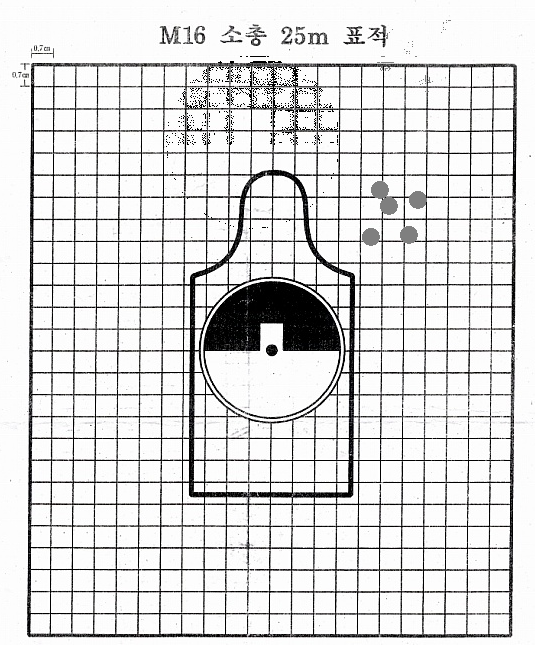
\includegraphics{images/bias_1.png}
\caption{mifeel\_gunfeel}
\end{figure}

    \begin{center}\rule{0.5\linewidth}{\linethickness}\end{center}

\begin{itemize}
\tightlist
\item
  \(y = 2x\)
\end{itemize}

    \begin{Verbatim}[commandchars=\\\{\}]
{\color{incolor}In [{\color{incolor}61}]:} \PY{n}{examples}\PY{o}{.}\PY{n}{draw\PYZus{}without\PYZus{}bias}\PY{p}{(}\PY{p}{)}
\end{Verbatim}


    \begin{center}
    \adjustimage{max size={0.9\linewidth}{0.9\paperheight}}{output_91_0.png}
    \end{center}
    { \hspace*{\fill} \\}
    
    \begin{center}\rule{0.5\linewidth}{\linethickness}\end{center}

\begin{itemize}
\tightlist
\item
  \(y=2x-4\)
\end{itemize}

    \begin{Verbatim}[commandchars=\\\{\}]
{\color{incolor}In [{\color{incolor}62}]:} \PY{n}{examples}\PY{o}{.}\PY{n}{draw\PYZus{}with\PYZus{}bias}\PY{p}{(}\PY{p}{)}
\end{Verbatim}


    \begin{center}
    \adjustimage{max size={0.9\linewidth}{0.9\paperheight}}{output_93_0.png}
    \end{center}
    { \hspace*{\fill} \\}
    
    \hypertarget{complete-network}{%
\subsubsection{Complete Network}\label{complete-network}}

    \texttt{Input}과 \texttt{Layer}, \texttt{Activation}을 활용하여 간단한
\texttt{Multi\ Layer\ Perceptron} 모델을 생성해 보자.

    \begin{Verbatim}[commandchars=\\\{\}]
{\color{incolor}In [{\color{incolor}63}]:} \PY{c+c1}{\PYZsh{} Input Layer}
         \PY{n}{input\PYZus{}layer} \PY{o}{=} \PY{n}{arr\PYZus{}x1}
         
         
         \PY{c+c1}{\PYZsh{} Hidden Layer}
         \PY{n}{hidden\PYZus{}layer\PYZus{}1}\PY{p}{,} \PY{n}{w1} \PY{o}{=} \PY{n}{dense\PYZus{}layer}\PY{p}{(}
             \PY{n}{input\PYZus{}layer}\PY{p}{,}
             \PY{n}{output\PYZus{}dim}\PY{o}{=}\PY{l+m+mi}{4}\PY{p}{,}
             \PY{n}{seed}\PY{o}{=}\PY{l+m+mi}{4}\PY{p}{,}
             \PY{n}{name}\PY{o}{=}\PY{l+s+s1}{\PYZsq{}}\PY{l+s+s1}{fc1\PYZus{}layer}\PY{l+s+s1}{\PYZsq{}}\PY{p}{,}
         \PY{p}{)}
         \PY{n}{activated\PYZus{}1} \PY{o}{=} \PY{n}{sigmoid}\PY{p}{(}\PY{n}{hidden\PYZus{}layer\PYZus{}1}\PY{p}{)}
         
         
         \PY{c+c1}{\PYZsh{} Output Layer}
         \PY{n}{hidden\PYZus{}layer\PYZus{}2}\PY{p}{,} \PY{n}{w2} \PY{o}{=} \PY{n}{dense\PYZus{}layer}\PY{p}{(}
             \PY{n}{hidden\PYZus{}layer\PYZus{}1}\PY{p}{,}
             \PY{n}{output\PYZus{}dim}\PY{o}{=}\PY{l+m+mi}{2}\PY{p}{,}
             \PY{n}{seed}\PY{o}{=}\PY{l+m+mi}{3}\PY{p}{,}
             \PY{n}{name}\PY{o}{=}\PY{l+s+s1}{\PYZsq{}}\PY{l+s+s1}{fc2\PYZus{}layer}\PY{l+s+s1}{\PYZsq{}}\PY{p}{,}
         \PY{p}{)}
         \PY{n}{activated\PYZus{}2} \PY{o}{=} \PY{n}{sigmoid}\PY{p}{(}\PY{n}{hidden\PYZus{}layer\PYZus{}2}\PY{p}{)}
\end{Verbatim}


    \begin{Verbatim}[commandchars=\\\{\}]
fc1\_layer
==========================================================================================================
|  Input               |   Weight                   |   Output                                           |
|  (1, 3)              |   (3, 4)                   |   (1, 4)                                           |
==========================================================================================================
|  [[0.93 0.65 0.03]]  |   [[0.97 0.55 0.97 0.71]   |   [[1.36459999 0.6674     1.56249998 0.6728    ]]  |
|                      |    [0.7  0.22 0.98 0.01]   |                                                    |
|                      |    [0.25 0.43 0.78 0.2 ]]  |                                                    |
==========================================================================================================
sigmoid
==========================================================================================================
|  Raw                                              |   Activated                                        |
|  (1, 4)                                           |   (1, 4)                                           |
==========================================================================================================
|  [[1.36459999 0.6674     1.56249998 0.6728    ]]  |   [[0.7965063  0.66092073 0.82671179 0.66212984]]  |
==========================================================================================================
fc2\_layer
=======================================================================================================
|  Input                                            |   Weight         |   Output                     |
|  (1, 4)                                           |   (4, 2)         |   (1, 2)                     |
=======================================================================================================
|  [[1.36459999 0.6674     1.56249998 0.6728    ]]  |   [[0.55 0.71]   |   [[2.42216498 2.85677798]]  |
|                                                   |    [0.29 0.51]   |                              |
|                                                   |    [0.89 0.9 ]   |                              |
|                                                   |    [0.13 0.21]]  |                              |
=======================================================================================================
sigmoid
==============================================================
|  Raw                        |   Activated                  |
|  (1, 2)                     |   (1, 2)                     |
==============================================================
|  [[2.42216498 2.85677798]]  |   [[0.91850195 0.94566799]]  |
==============================================================

    \end{Verbatim}

    \begin{Verbatim}[commandchars=\\\{\}]
{\color{incolor}In [{\color{incolor}64}]:} \PY{n}{hidden\PYZus{}layer\PYZus{}2}
\end{Verbatim}


\begin{Verbatim}[commandchars=\\\{\}]
{\color{outcolor}Out[{\color{outcolor}64}]:} array([[2.42216498, 2.85677798]])
\end{Verbatim}
            
    \begin{Verbatim}[commandchars=\\\{\}]
{\color{incolor}In [{\color{incolor}65}]:} \PY{n}{activated\PYZus{}2}
\end{Verbatim}


\begin{Verbatim}[commandchars=\\\{\}]
{\color{outcolor}Out[{\color{outcolor}65}]:} array([[0.91850195, 0.94566799]])
\end{Verbatim}
            
    \hypertarget{batch}{%
\subsubsection{Batch}\label{batch}}

 이제 Batch에 대해 알아보자. Batch는 한번 학습에 이용하는 샘플 단위를
말한다. 전체 Input의 개수가 10이고 \texttt{batch\_size}가 2일 경우,
\(\space\space\) \(\leftarrow\) input\_size: 10, batch\_size: 2
부분집합인 2개씩을 꺼내어 1번 학습에 활용하게 되고 \(\space\space\)
\(\leftarrow\) step\_num: 1 (누적학습횟수) 총 5번 학습하면 전체 Input을
다 학습하게 된다. \(\space\space\) \(\leftarrow\) batch\_nu: 5
(학습횟수) 이렇게 Input을 한번 다 보는 경우를 1 epoch이라 하며,
\(\space\space\) \(\leftarrow\) epoch\_num: 1

10 epoch로 학습하는 경우\\
\texttt{batch\_num}은 5, \texttt{step\_num}은 50이 된다.

 \(\space\) \(\space 1 \space Epoch,\) \begin{equation}
\begin{bmatrix} 1st \space Batch \times \color{red}3 \end{bmatrix}
\overbrace{ \begin{bmatrix} \color{red}3 \times \color{blue}4 \end{bmatrix} }^{1st Layer}
\overbrace{ \begin{bmatrix} \color{blue}4 \times 2 \end{bmatrix} }^{2nd Layer}
= \begin{bmatrix} 1st \space Batch \times 2 \end{bmatrix}
\Rightarrow 1st \space Backpropagation
\end{equation}\\
\begin{equation}
\begin{bmatrix} 2nd \space Batch \times \color{red}3 \end{bmatrix}
\overbrace{ \begin{bmatrix} \color{red}3 \times \color{blue}4 \end{bmatrix} }^{1st Layer}
\overbrace{ \begin{bmatrix} \color{blue}4 \times 2 \end{bmatrix} }^{2nd Layer}
= \begin{bmatrix} 2nd \space Batch \times 2 \end{bmatrix}
\Rightarrow 2nd \space Backpropagation
\end{equation}\\
\[\vdots\] \begin{equation}
\begin{bmatrix} 5th \space Batch \times \color{red}3 \end{bmatrix}
\overbrace{ \begin{bmatrix} \color{red}3 \times \color{blue}4 \end{bmatrix} }^{1st Layer}
\overbrace{ \begin{bmatrix} \color{blue}4 \times 2 \end{bmatrix} }^{2nd Layer}
= \begin{bmatrix} 5th \space Batch \times 2 \end{bmatrix}
\Rightarrow 5th \space Backpropagation
\end{equation} \(\space\)

학습할 때는 주어진 \texttt{input\_size}에 대해 \texttt{batch\_size}와
\texttt{epoch\_num}을 지정한다. 이제, 딥러닝 모델이 Input을 어떻게
읽어들이는 지 알 수 있다.

\(\divideontimes\) Batch란: 1번 학습에 활용하는 Input의 부분집합 단위

 \[Batch \space num = \frac {Input \space size}{Batch \space size}\]

\[1 \space Epoch = Batch \space size \times Batch \space num\]

\[ Step \space num = Epoch \space num \times Batch \space num\]\\

    \begin{Verbatim}[commandchars=\\\{\}]
{\color{incolor}In [{\color{incolor}66}]:} \PY{c+c1}{\PYZsh{} Input Layer}
         \PY{n}{input\PYZus{}layer} \PY{o}{=} \PY{n}{arr\PYZus{}x1}
         
         
         \PY{c+c1}{\PYZsh{} Hidden Layer}
         \PY{n}{hidden\PYZus{}layer\PYZus{}1}\PY{p}{,} \PY{n}{w1} \PY{o}{=} \PY{n}{dense\PYZus{}layer}\PY{p}{(}
             \PY{n}{input\PYZus{}layer}\PY{p}{,}
             \PY{n}{output\PYZus{}dim}\PY{o}{=}\PY{l+m+mi}{4}\PY{p}{,}
             \PY{n}{seed}\PY{o}{=}\PY{l+m+mi}{4}\PY{p}{,}
             \PY{n}{name}\PY{o}{=}\PY{l+s+s1}{\PYZsq{}}\PY{l+s+s1}{fc1\PYZus{}layer}\PY{l+s+s1}{\PYZsq{}}\PY{p}{,}
         \PY{p}{)}
         \PY{n}{activated\PYZus{}1} \PY{o}{=} \PY{n}{sigmoid}\PY{p}{(}\PY{n}{hidden\PYZus{}layer\PYZus{}1}\PY{p}{)}
         
         
         \PY{c+c1}{\PYZsh{} Output Layer}
         \PY{n}{hidden\PYZus{}layer\PYZus{}2}\PY{p}{,} \PY{n}{w2} \PY{o}{=} \PY{n}{dense\PYZus{}layer}\PY{p}{(}
             \PY{n}{hidden\PYZus{}layer\PYZus{}1}\PY{p}{,}
             \PY{n}{output\PYZus{}dim}\PY{o}{=}\PY{l+m+mi}{2}\PY{p}{,}
             \PY{n}{seed}\PY{o}{=}\PY{l+m+mi}{3}\PY{p}{,}
             \PY{n}{name}\PY{o}{=}\PY{l+s+s1}{\PYZsq{}}\PY{l+s+s1}{fc2\PYZus{}layer}\PY{l+s+s1}{\PYZsq{}}\PY{p}{,}
         \PY{p}{)}
         \PY{n}{activated\PYZus{}2} \PY{o}{=} \PY{n}{sigmoid}\PY{p}{(}\PY{n}{hidden\PYZus{}layer\PYZus{}2}\PY{p}{)}
\end{Verbatim}


    \begin{Verbatim}[commandchars=\\\{\}]
fc1\_layer
==========================================================================================================
|  Input               |   Weight                   |   Output                                           |
|  (1, 3)              |   (3, 4)                   |   (1, 4)                                           |
==========================================================================================================
|  [[0.93 0.65 0.03]]  |   [[0.97 0.55 0.97 0.71]   |   [[1.36459999 0.6674     1.56249998 0.6728    ]]  |
|                      |    [0.7  0.22 0.98 0.01]   |                                                    |
|                      |    [0.25 0.43 0.78 0.2 ]]  |                                                    |
==========================================================================================================
sigmoid
==========================================================================================================
|  Raw                                              |   Activated                                        |
|  (1, 4)                                           |   (1, 4)                                           |
==========================================================================================================
|  [[1.36459999 0.6674     1.56249998 0.6728    ]]  |   [[0.7965063  0.66092073 0.82671179 0.66212984]]  |
==========================================================================================================
fc2\_layer
=======================================================================================================
|  Input                                            |   Weight         |   Output                     |
|  (1, 4)                                           |   (4, 2)         |   (1, 2)                     |
=======================================================================================================
|  [[1.36459999 0.6674     1.56249998 0.6728    ]]  |   [[0.55 0.71]   |   [[2.42216498 2.85677798]]  |
|                                                   |    [0.29 0.51]   |                              |
|                                                   |    [0.89 0.9 ]   |                              |
|                                                   |    [0.13 0.21]]  |                              |
=======================================================================================================
sigmoid
==============================================================
|  Raw                        |   Activated                  |
|  (1, 2)                     |   (1, 2)                     |
==============================================================
|  [[2.42216498 2.85677798]]  |   [[0.91850195 0.94566799]]  |
==============================================================

    \end{Verbatim}

    \hypertarget{loss-function}{%
\subsubsection{Loss Function}\label{loss-function}}

    \texttt{Cost\ Function} 혹은 \texttt{Objective\ Function}으로도
불린다.\\
예측값과 실제값의 차이를 \texttt{Error} 또는 \texttt{Cost}라고 부르는데
이 \texttt{Error}의 측정방법이 곧 \texttt{Loss\ Function}이다.\\
'모델이 학습한다'는 의미는, 이 값을 최소화 하는 방향으로 \(w\) 와 \(b\)
를 업데이트 한다는 뜻이다. \\

* \texttt{accuracy}를 목적함수로 사용할 경우, 업데이트함에 따라 값이
불연속적으로 변하기 때문에 부적합.

    \hypertarget{mean-square-error}{%
\paragraph{Mean Square Error}\label{mean-square-error}}

    제일 기본적인 \texttt{Loss\ Function}이며,\\
값의 차이를 제곱하여 그 크기 값의 평균을 계산한다.

 \[loss = \mathcal{L}(\hat{y}, y) = (\hat y^{(i)} - y^{(i)})^2\]
\[MSE = \frac {1}{m} \sum_{i=1}^{m}(\hat y_{i} - y_{i})^2 \]

    \begin{Verbatim}[commandchars=\\\{\}]
{\color{incolor}In [{\color{incolor}67}]:} \PY{k}{def} \PY{n+nf}{mean\PYZus{}squared\PYZus{}error}\PY{p}{(}\PY{n}{logits}\PY{p}{,} \PY{n}{real}\PY{p}{)}\PY{p}{:}
             
             
             \PY{c+c1}{\PYZsh{}==== Essential ========================================================\PYZsh{}}
             
             \PY{n}{err} \PY{o}{=} \PY{p}{(}\PY{p}{(}\PY{n}{logits} \PY{o}{\PYZhy{}} \PY{n}{real}\PY{p}{)} \PY{o}{*}\PY{o}{*} \PY{l+m+mi}{2}\PY{p}{)}\PY{o}{.}\PY{n}{mean}\PY{p}{(}\PY{p}{)}
             
             \PY{c+c1}{\PYZsh{}=======================================================================\PYZsh{}}
         
         
             \PY{k}{return} \PY{n}{err}
\end{Verbatim}


    \begin{Verbatim}[commandchars=\\\{\}]
{\color{incolor}In [{\color{incolor}68}]:} \PY{n}{mean\PYZus{}squared\PYZus{}error}\PY{p}{(}\PY{n}{activated\PYZus{}2}\PY{p}{,} \PY{n}{arr\PYZus{}y1}\PY{p}{)}
\end{Verbatim}


\begin{Verbatim}[commandchars=\\\{\}]
{\color{outcolor}Out[{\color{outcolor}68}]:} 0.0744360007255992
\end{Verbatim}
            
    \hypertarget{training}{%
\subsubsection{Training}\label{training}}

    \hypertarget{gradient-descent}{%
\paragraph{Gradient Descent}\label{gradient-descent}}

\texttt{Gradient}는 `경사도' 라는 뜻이며, \texttt{Gradient\ Descent}를
산을 내려가는 과정에 비유할 수 있다.

산 속에서 길을 잃었다고 생각해 보자.

\begin{enumerate}
\def\labelenumi{\arabic{enumi}.}
\item
  길찾기\\
  산을 빠져나오기 위해서는 산의 경사와 반대 방향으로 내려와야 한다.\\
  이렇게 길을 찾는 방법이 `Gradient Descent' 이다.
\item
  중간 골짜기\\
  시야가 좁거나 지도가 조금밖에 없을 경우,\\
  경사에 의존해서 내려갈 수는 있지만 이대로 가면 목적지가 나올 지 확신할
  수 없다.\\
  귀퉁이 골짜기에 도착해서 영원히 헤맬 수도 있다.\\
  이 때 우리는 `국소 최적해(Local Minima)'를 찾았다고 한다.
\item
  최종 목적지\\
  시야가 넓거나 산길에 대한 정보를 잘 알고 있는 경우, 또는 운이 좋으면\\
  가야할 곳을 잘 알고 때로는 다시 봉우리를 오르기도 하면서 목적지에
  도착할 수 있다.\\
  이 때 우리는 `전역 최적해(Global Minimum)'를 찾았다고 한다.
\item
  보폭\\
  보폭이 넓으면, 성큼성큼 갈 수는 있겠지만 너무 빨라서 길을 지나칠 수
  있다.\\
  보폭이 좁으면, 목적지를 잘 알아도 너무 느려서 가다 지칠 수 있다.\\
  가야할 곳을 잘 알고 때로는 다시 봉우리를 오르기도 하면서 목적지에
  도착할 수 있다.\\
  이 보폭이 `학습률(Learning Rate)'이다.
\end{enumerate}

    \begin{Verbatim}[commandchars=\\\{\}]
{\color{incolor}In [{\color{incolor}100}]:} \PY{n}{examples}\PY{o}{.}\PY{n}{gradient\PYZus{}plot\PYZus{}a}\PY{p}{(}\PY{p}{)}
          \PY{n}{examples}\PY{o}{.}\PY{n}{gradient\PYZus{}plot\PYZus{}b}\PY{p}{(}\PY{p}{)}
\end{Verbatim}


    \begin{Verbatim}[commandchars=\\\{\}]
/opt/conda/envs/tf-py36/lib/python3.6/site-packages/matplotlib/figure.py:457: UserWarning: matplotlib is currently using a non-GUI backend, so cannot show the figure
  "matplotlib is currently using a non-GUI backend, "
/opt/conda/envs/tf-py36/lib/python3.6/site-packages/matplotlib/figure.py:457: UserWarning: matplotlib is currently using a non-GUI backend, so cannot show the figure
  "matplotlib is currently using a non-GUI backend, "

    \end{Verbatim}

    \begin{center}
    \adjustimage{max size={0.9\linewidth}{0.9\paperheight}}{output_109_1.png}
    \end{center}
    { \hspace*{\fill} \\}
    
    \begin{center}
    \adjustimage{max size={0.9\linewidth}{0.9\paperheight}}{output_109_2.png}
    \end{center}
    { \hspace*{\fill} \\}
    
    \hypertarget{forward-propagation}{%
\paragraph{Forward-propagation}\label{forward-propagation}}

    \begin{itemize}
\tightlist
\item
  Dense Layer
\end{itemize}

    \begin{itemize}
\tightlist
\item
  Activation Layer
\end{itemize}

    \hypertarget{forward-propagation}{%
\subparagraph{Forward-propagation}\label{forward-propagation}}

    \begin{Verbatim}[commandchars=\\\{\}]
{\color{incolor}In [{\color{incolor}101}]:} \PY{k+kn}{from} \PY{n+nn}{src}\PY{n+nn}{.}\PY{n+nn}{layers} \PY{k}{import} \PY{n}{dense\PYZus{}layer}\PY{p}{,} \PY{n}{sigmoid}\PY{p}{,} \PY{n}{tanh}
          
          
          \PY{k}{def} \PY{n+nf}{forward\PYZus{}propagation}\PY{p}{(}
              \PY{n}{input\PYZus{}x}\PY{p}{,}
              \PY{n}{weight\PYZus{}dict}\PY{o}{=}\PY{k+kc}{None}\PY{p}{,}
              \PY{n}{print\PYZus{}ok}\PY{o}{=}\PY{k+kc}{True}\PY{p}{,}
              \PY{p}{)}\PY{p}{:}
          
              \PY{k}{if} \PY{n}{weight\PYZus{}dict} \PY{o+ow}{is} \PY{k+kc}{None}\PY{p}{:}
                  \PY{n}{weight\PYZus{}dict} \PY{o}{=} \PY{p}{\PYZob{}}
                      \PY{l+s+s1}{\PYZsq{}}\PY{l+s+s1}{w1}\PY{l+s+s1}{\PYZsq{}}\PY{p}{:} \PY{k+kc}{None}\PY{p}{,}
                      \PY{l+s+s1}{\PYZsq{}}\PY{l+s+s1}{b1}\PY{l+s+s1}{\PYZsq{}}\PY{p}{:} \PY{k+kc}{None}\PY{p}{,}
                      \PY{l+s+s1}{\PYZsq{}}\PY{l+s+s1}{w2}\PY{l+s+s1}{\PYZsq{}}\PY{p}{:} \PY{k+kc}{None}\PY{p}{,}
                      \PY{l+s+s1}{\PYZsq{}}\PY{l+s+s1}{b2}\PY{l+s+s1}{\PYZsq{}}\PY{p}{:} \PY{k+kc}{None}\PY{p}{,}
                  \PY{p}{\PYZcb{}}
              
              \PY{n}{w1} \PY{o}{=} \PY{n}{weight\PYZus{}dict}\PY{p}{[}\PY{l+s+s1}{\PYZsq{}}\PY{l+s+s1}{w1}\PY{l+s+s1}{\PYZsq{}}\PY{p}{]}
              \PY{n}{b1} \PY{o}{=} \PY{n}{weight\PYZus{}dict}\PY{p}{[}\PY{l+s+s1}{\PYZsq{}}\PY{l+s+s1}{b1}\PY{l+s+s1}{\PYZsq{}}\PY{p}{]}
              \PY{n}{w2} \PY{o}{=} \PY{n}{weight\PYZus{}dict}\PY{p}{[}\PY{l+s+s1}{\PYZsq{}}\PY{l+s+s1}{w2}\PY{l+s+s1}{\PYZsq{}}\PY{p}{]}
              \PY{n}{b2} \PY{o}{=} \PY{n}{weight\PYZus{}dict}\PY{p}{[}\PY{l+s+s1}{\PYZsq{}}\PY{l+s+s1}{b2}\PY{l+s+s1}{\PYZsq{}}\PY{p}{]}
          
              
              \PY{c+c1}{\PYZsh{}==== Essential ========================================================\PYZsh{}}
          
              \PY{c+c1}{\PYZsh{}\PYZsh{}\PYZsh{}\PYZsh{}\PYZsh{} LAYER (Forward\PYZhy{}propagation) \PYZsh{}\PYZsh{}\PYZsh{}\PYZsh{}\PYZsh{}}
          
              \PY{c+c1}{\PYZsh{} Input Layer}
              \PY{n}{input\PYZus{}layer} \PY{o}{=} \PY{n}{input\PYZus{}x}
          
              \PY{c+c1}{\PYZsh{} Hidden Layer}
              \PY{n}{hidden\PYZus{}layer\PYZus{}1}\PY{p}{,} \PY{n}{w1}\PY{p}{,} \PY{n}{b1} \PY{o}{=} \PY{n}{dense\PYZus{}layer}\PY{p}{(}
                  \PY{n}{input\PYZus{}layer}\PY{p}{,}
                  \PY{n}{output\PYZus{}dim}\PY{o}{=}\PY{l+m+mi}{4}\PY{p}{,}
                  \PY{n}{weight}\PY{o}{=}\PY{n}{w1}\PY{p}{,}
                  \PY{n}{bias}\PY{o}{=}\PY{n}{b1}\PY{p}{,}
                  \PY{n}{seed}\PY{o}{=}\PY{l+m+mi}{4}\PY{p}{,}
                  \PY{n}{name}\PY{o}{=}\PY{l+s+s1}{\PYZsq{}}\PY{l+s+s1}{fc1\PYZus{}layer}\PY{l+s+s1}{\PYZsq{}}\PY{p}{,}
                  \PY{n}{print\PYZus{}ok}\PY{o}{=}\PY{n}{print\PYZus{}ok}\PY{p}{,}
              \PY{p}{)}
              \PY{n}{activated\PYZus{}1} \PY{o}{=} \PY{n}{sigmoid}\PY{p}{(}\PY{n}{hidden\PYZus{}layer\PYZus{}1}\PY{p}{,} \PY{n}{print\PYZus{}ok}\PY{o}{=}\PY{n}{print\PYZus{}ok}\PY{p}{)}
          
              \PY{c+c1}{\PYZsh{} Output Layer}
              \PY{n}{hidden\PYZus{}layer\PYZus{}2}\PY{p}{,} \PY{n}{w2}\PY{p}{,} \PY{n}{b2} \PY{o}{=} \PY{n}{dense\PYZus{}layer}\PY{p}{(}
                  \PY{n}{hidden\PYZus{}layer\PYZus{}1}\PY{p}{,}
                  \PY{n}{output\PYZus{}dim}\PY{o}{=}\PY{l+m+mi}{2}\PY{p}{,}
                  \PY{n}{weight}\PY{o}{=}\PY{n}{w2}\PY{p}{,}
                  \PY{n}{bias}\PY{o}{=}\PY{n}{b2}\PY{p}{,}
                  \PY{n}{seed}\PY{o}{=}\PY{l+m+mi}{3}\PY{p}{,}
                  \PY{n}{name}\PY{o}{=}\PY{l+s+s1}{\PYZsq{}}\PY{l+s+s1}{fc2\PYZus{}layer}\PY{l+s+s1}{\PYZsq{}}\PY{p}{,}
                  \PY{n}{print\PYZus{}ok}\PY{o}{=}\PY{n}{print\PYZus{}ok}\PY{p}{,}
              \PY{p}{)}
              \PY{n}{activated\PYZus{}2} \PY{o}{=} \PY{n}{sigmoid}\PY{p}{(}\PY{n}{hidden\PYZus{}layer\PYZus{}2}\PY{p}{,} \PY{n}{print\PYZus{}ok}\PY{o}{=}\PY{n}{print\PYZus{}ok}\PY{p}{)}
              
              \PY{c+c1}{\PYZsh{}=======================================================================\PYZsh{}}
              
              
              \PY{k}{if} \PY{n}{print\PYZus{}ok}\PY{p}{:}
                  \PY{n+nb}{print}\PY{p}{(}\PY{n}{f}\PY{l+s+s1}{\PYZsq{}}\PY{l+s+se}{\PYZbs{}n}\PY{l+s+s1}{= Input =}\PY{l+s+se}{\PYZbs{}n}\PY{l+s+si}{\PYZob{}input\PYZus{}layer\PYZcb{}}\PY{l+s+s1}{\PYZsq{}}\PY{p}{)}
                  \PY{n+nb}{print}\PY{p}{(}\PY{n}{f}\PY{l+s+s1}{\PYZsq{}}\PY{l+s+se}{\PYZbs{}n}\PY{l+s+s1}{= 1 Layer =}\PY{l+s+se}{\PYZbs{}n}\PY{l+s+si}{\PYZob{}hidden\PYZus{}layer\PYZus{}1\PYZcb{}}\PY{l+s+se}{\PYZbs{}n}\PY{l+s+si}{\PYZob{}activated\PYZus{}1\PYZcb{}}\PY{l+s+s1}{\PYZsq{}}\PY{p}{)}
                  \PY{n+nb}{print}\PY{p}{(}\PY{n}{f}\PY{l+s+s1}{\PYZsq{}}\PY{l+s+se}{\PYZbs{}n}\PY{l+s+s1}{= 2 Layer =}\PY{l+s+se}{\PYZbs{}n}\PY{l+s+si}{\PYZob{}hidden\PYZus{}layer\PYZus{}2\PYZcb{}}\PY{l+s+s1}{\PYZsq{}}\PY{p}{)}
                  \PY{n+nb}{print}\PY{p}{(}\PY{n}{f}\PY{l+s+s1}{\PYZsq{}}\PY{l+s+se}{\PYZbs{}n}\PY{l+s+s1}{= Output =}\PY{l+s+se}{\PYZbs{}n}\PY{l+s+si}{\PYZob{}activated\PYZus{}2\PYZcb{}}\PY{l+s+s1}{\PYZsq{}}\PY{p}{)}
          
          
              \PY{n}{weight\PYZus{}dict}\PY{p}{[}\PY{l+s+s1}{\PYZsq{}}\PY{l+s+s1}{w1}\PY{l+s+s1}{\PYZsq{}}\PY{p}{]} \PY{o}{=} \PY{n}{w1}
              \PY{n}{weight\PYZus{}dict}\PY{p}{[}\PY{l+s+s1}{\PYZsq{}}\PY{l+s+s1}{b1}\PY{l+s+s1}{\PYZsq{}}\PY{p}{]} \PY{o}{=} \PY{n}{b1}
              \PY{n}{weight\PYZus{}dict}\PY{p}{[}\PY{l+s+s1}{\PYZsq{}}\PY{l+s+s1}{l1}\PY{l+s+s1}{\PYZsq{}}\PY{p}{]} \PY{o}{=} \PY{n}{hidden\PYZus{}layer\PYZus{}1}
              \PY{n}{weight\PYZus{}dict}\PY{p}{[}\PY{l+s+s1}{\PYZsq{}}\PY{l+s+s1}{a1}\PY{l+s+s1}{\PYZsq{}}\PY{p}{]} \PY{o}{=} \PY{n}{activated\PYZus{}1}
              
              
              \PY{n}{weight\PYZus{}dict}\PY{p}{[}\PY{l+s+s1}{\PYZsq{}}\PY{l+s+s1}{w2}\PY{l+s+s1}{\PYZsq{}}\PY{p}{]} \PY{o}{=} \PY{n}{w2}
              \PY{n}{weight\PYZus{}dict}\PY{p}{[}\PY{l+s+s1}{\PYZsq{}}\PY{l+s+s1}{b2}\PY{l+s+s1}{\PYZsq{}}\PY{p}{]} \PY{o}{=} \PY{n}{b2}
              \PY{n}{weight\PYZus{}dict}\PY{p}{[}\PY{l+s+s1}{\PYZsq{}}\PY{l+s+s1}{l2}\PY{l+s+s1}{\PYZsq{}}\PY{p}{]} \PY{o}{=} \PY{n}{hidden\PYZus{}layer\PYZus{}2}
              \PY{n}{weight\PYZus{}dict}\PY{p}{[}\PY{l+s+s1}{\PYZsq{}}\PY{l+s+s1}{a2}\PY{l+s+s1}{\PYZsq{}}\PY{p}{]} \PY{o}{=} \PY{n}{activated\PYZus{}2}
          
              \PY{k}{return} \PY{n}{activated\PYZus{}2}\PY{p}{,} \PY{n}{weight\PYZus{}dict}
\end{Verbatim}


    \begin{Verbatim}[commandchars=\\\{\}]
{\color{incolor}In [{\color{incolor}102}]:} \PY{n}{output}\PY{p}{,} \PY{n}{w\PYZus{}dict} \PY{o}{=} \PY{n}{forward\PYZus{}propagation}\PY{p}{(}\PY{n}{arr\PYZus{}x1}\PY{p}{)}
\end{Verbatim}


    \begin{Verbatim}[commandchars=\\\{\}]
fc1\_layer:	(1, 3) -> (1, 4)
sigmoid
==========================================================================================================
|  Raw                                              |   Activated                                        |
|  (1, 4)                                           |   (1, 4)                                           |
==========================================================================================================
|  [[2.22459999 1.6474     1.72249998 1.2728    ]]  |   [[0.90243695 0.83853934 0.84845057 0.78122169]]  |
==========================================================================================================
fc2\_layer:	(1, 4) -> (1, 2)
sigmoid
==============================================================
|  Raw                        |   Activated                  |
|  (1, 2)                     |   (1, 2)                     |
==============================================================
|  [[3.44976498 4.67717798]]  |   [[0.96922413 0.99078055]]  |
==============================================================

= Input =
[[0.93 0.65 0.03]]

= 1 Layer =
[[2.22459999 1.6474     1.72249998 1.2728    ]]
[[0.90243695 0.83853934 0.84845057 0.78122169]]

= 2 Layer =
[[3.44976498 4.67717798]]

= Output =
[[0.96922413 0.99078055]]

    \end{Verbatim}

    \hypertarget{backpropagation}{%
\paragraph{Backpropagation}\label{backpropagation}}

\(\divideontimes\) 역전파(Backpropagation):

마지막 Output과 실제 값과의 차이( \(Loss\) )로 배운 경험을\\
내부 \(Weight\)에 골고루 Feedback하는 과정.

\(\divideontimes\) Chain Rule: 합성함수의 도함수에 대한 공식이다. \[
z = g(f((x)) \space 일 \space 때 \\
\space \\
\frac{\partial z}{\partial x} = \frac{\partial z}{\partial y}\frac{\partial y}{\partial x}
\]

모델은 Layer들 간의 합성으로 이루어져 있다.\\
즉, 모델 전체를 미분한 값은 Layer 각각 미분값의 곱과 같다.

\[
\frac{\partial z}{\partial w} = \frac{\partial z}{\partial y}\frac{\partial y}{\partial x}\frac{\partial x}{\partial w}
\]


\[ \frac{\partial J}{\partial \theta} = \lim_{\varepsilon \to 0} \frac{J(\theta + \varepsilon) - J(\theta - \varepsilon)}{2 \varepsilon}\]

\(J\)는 \(Error\)를, \(\theta\)는 \(Weight\)를 의미한다.\\
즉, \(\frac{\partial J}{\partial \theta}\)는 \(Weight\) 변화량 대비
\(Error\) 값의 변화량을 의미한다.

 \[
J = MSE = \frac{1}{m}\sum\limits_{i=1}^m {(\hat{y} - y)^2}
\]

    \(\divideontimes\) Derivative of Sigmoid 비선형함수로 `sigmoid'가 자주
쓰이는 이유 중 하나는 도함수가 간단하기 때문이다.

\begin{array}{ll} \hline
Name
&
Formula
&
Derivative
\\ \hline
sigmoid
&
\sigma(x) = \dfrac{1}{1+e^{-x}}
&
\sigma(x)(1 - \sigma(x))
\\ \hline
tanh
&
2\sigma(2x) - 1
&
1-\tanh(x)^2
\\ \hline
\end{array}

    \begin{Verbatim}[commandchars=\\\{\}]
{\color{incolor}In [{\color{incolor}103}]:} \PY{k}{def} \PY{n+nf}{d\PYZus{}sigmoid}\PY{p}{(}\PY{n}{y}\PY{p}{)}\PY{p}{:}
              \PY{k}{return} \PY{n}{y} \PY{o}{*} \PY{p}{(}\PY{l+m+mi}{1} \PY{o}{\PYZhy{}} \PY{n}{y}\PY{p}{)}
\end{Verbatim}


    \hypertarget{backpropagation-scratch}{%
\subparagraph{Backpropagation (Scratch)}\label{backpropagation-scratch}}

    \begin{Verbatim}[commandchars=\\\{\}]
{\color{incolor}In [{\color{incolor}104}]:} \PY{k+kn}{from} \PY{n+nn}{src}\PY{n+nn}{.}\PY{n+nn}{layers} \PY{k}{import} \PY{n}{d\PYZus{}sigmoid}\PY{p}{,} \PY{n}{d\PYZus{}tanh}
          
          
          \PY{k}{def} \PY{n+nf}{backward\PYZus{}propagation\PYZus{}scratch}\PY{p}{(}
              \PY{n}{input\PYZus{}x}\PY{p}{,}
              \PY{n}{input\PYZus{}y}\PY{p}{,}
              \PY{n}{weight\PYZus{}dict}\PY{o}{=}\PY{k+kc}{None}\PY{p}{,}
              \PY{n}{learning\PYZus{}rate}\PY{o}{=}\PY{l+m+mf}{5e\PYZhy{}2}\PY{p}{,}
              \PY{n}{print\PYZus{}ok}\PY{o}{=}\PY{k+kc}{True}\PY{p}{,}
              \PY{p}{)}\PY{p}{:}
              
              \PY{n}{m} \PY{o}{=} \PY{n}{input\PYZus{}dim} \PY{o}{=} \PY{n}{input\PYZus{}x}\PY{o}{.}\PY{n}{shape}\PY{p}{[}\PY{o}{\PYZhy{}}\PY{l+m+mi}{1}\PY{p}{]}
          
              \PY{n}{w1} \PY{o}{=} \PY{n}{weight\PYZus{}dict}\PY{p}{[}\PY{l+s+s1}{\PYZsq{}}\PY{l+s+s1}{w1}\PY{l+s+s1}{\PYZsq{}}\PY{p}{]}
              \PY{n}{b1} \PY{o}{=} \PY{n}{weight\PYZus{}dict}\PY{p}{[}\PY{l+s+s1}{\PYZsq{}}\PY{l+s+s1}{b1}\PY{l+s+s1}{\PYZsq{}}\PY{p}{]}
              \PY{n}{l1} \PY{o}{=} \PY{n}{weight\PYZus{}dict}\PY{p}{[}\PY{l+s+s1}{\PYZsq{}}\PY{l+s+s1}{l1}\PY{l+s+s1}{\PYZsq{}}\PY{p}{]}
              \PY{n}{a1} \PY{o}{=} \PY{n}{weight\PYZus{}dict}\PY{p}{[}\PY{l+s+s1}{\PYZsq{}}\PY{l+s+s1}{a1}\PY{l+s+s1}{\PYZsq{}}\PY{p}{]}
              
              \PY{n}{w2} \PY{o}{=} \PY{n}{weight\PYZus{}dict}\PY{p}{[}\PY{l+s+s1}{\PYZsq{}}\PY{l+s+s1}{w2}\PY{l+s+s1}{\PYZsq{}}\PY{p}{]}
              \PY{n}{b2} \PY{o}{=} \PY{n}{weight\PYZus{}dict}\PY{p}{[}\PY{l+s+s1}{\PYZsq{}}\PY{l+s+s1}{b2}\PY{l+s+s1}{\PYZsq{}}\PY{p}{]}
              \PY{n}{l2} \PY{o}{=} \PY{n}{weight\PYZus{}dict}\PY{p}{[}\PY{l+s+s1}{\PYZsq{}}\PY{l+s+s1}{l2}\PY{l+s+s1}{\PYZsq{}}\PY{p}{]}
              \PY{n}{a2} \PY{o}{=} \PY{n}{weight\PYZus{}dict}\PY{p}{[}\PY{l+s+s1}{\PYZsq{}}\PY{l+s+s1}{a2}\PY{l+s+s1}{\PYZsq{}}\PY{p}{]}
              
              
              \PY{c+c1}{\PYZsh{}==== Essential ========================================================\PYZsh{}}
          
              \PY{c+c1}{\PYZsh{}\PYZsh{}\PYZsh{}\PYZsh{}\PYZsh{} LAYER (Back\PYZhy{}propagation) \PYZsh{}\PYZsh{}\PYZsh{}\PYZsh{}\PYZsh{}}
          
              \PY{c+c1}{\PYZsh{} Calculate Gradients}
              \PY{n}{err} \PY{o}{=} \PY{n}{a2} \PY{o}{\PYZhy{}} \PY{n}{input\PYZus{}y}
              \PY{n}{d\PYZus{}a2} \PY{o}{=} \PY{n}{err} \PY{o}{/} \PY{n}{d\PYZus{}sigmoid}\PY{p}{(}\PY{n}{a2}\PY{p}{)}
              \PY{n}{d\PYZus{}l2} \PY{o}{=} \PY{n}{a2} \PY{o}{\PYZhy{}} \PY{n}{input\PYZus{}y}
              \PY{n}{d\PYZus{}b2} \PY{o}{=} \PY{l+m+mf}{1.}\PY{o}{/}\PY{n}{m} \PY{o}{*} \PY{n}{np}\PY{o}{.}\PY{n}{sum}\PY{p}{(}\PY{n}{d\PYZus{}l2}\PY{o}{.}\PY{n}{T}\PY{p}{,} \PY{n}{axis}\PY{o}{=}\PY{l+m+mi}{1}\PY{p}{,} \PY{n}{keepdims}\PY{o}{=}\PY{k+kc}{False}\PY{p}{)}
              \PY{n}{d\PYZus{}o2} \PY{o}{=} \PY{n}{d\PYZus{}l2}
          
              \PY{n}{d\PYZus{}w2} \PY{o}{=} \PY{l+m+mf}{1.}\PY{o}{/}\PY{n}{m} \PY{o}{*} \PY{p}{(}\PY{n}{a1}\PY{o}{.}\PY{n}{T} \PY{o}{@} \PY{n}{d\PYZus{}o2}\PY{p}{)}
              \PY{n}{d\PYZus{}a1} \PY{o}{=} \PY{n}{d\PYZus{}o2} \PY{o}{@} \PY{n}{w2}\PY{o}{.}\PY{n}{T}
              \PY{n}{d\PYZus{}l1} \PY{o}{=} \PY{n}{d\PYZus{}sigmoid}\PY{p}{(}\PY{n}{a1}\PY{p}{)}
              \PY{n}{d\PYZus{}b1} \PY{o}{=} \PY{l+m+mf}{1.}\PY{o}{/}\PY{n}{m} \PY{o}{*} \PY{n}{np}\PY{o}{.}\PY{n}{sum}\PY{p}{(}\PY{n}{d\PYZus{}l1}\PY{o}{.}\PY{n}{T}\PY{p}{,} \PY{n}{axis}\PY{o}{=}\PY{l+m+mi}{1}\PY{p}{,} \PY{n}{keepdims}\PY{o}{=}\PY{k+kc}{False}\PY{p}{)}
              \PY{n}{d\PYZus{}o1} \PY{o}{=} \PY{n}{d\PYZus{}l1}
              \PY{n}{d\PYZus{}w1} \PY{o}{=} \PY{l+m+mf}{1.}\PY{o}{/}\PY{n}{m} \PY{o}{*} \PY{p}{(}\PY{n}{input\PYZus{}x}\PY{o}{.}\PY{n}{T} \PY{o}{@} \PY{n}{d\PYZus{}o1}\PY{p}{)}
          
              
              \PY{c+c1}{\PYZsh{} Update}
              \PY{n}{new\PYZus{}w1} \PY{o}{=} \PY{n}{w1} \PY{o}{\PYZhy{}} \PY{p}{(}\PY{n}{learning\PYZus{}rate} \PY{o}{*} \PY{n}{d\PYZus{}w1}\PY{p}{)}
              \PY{n}{new\PYZus{}b1} \PY{o}{=} \PY{n}{b1} \PY{o}{\PYZhy{}} \PY{p}{(}\PY{n}{learning\PYZus{}rate} \PY{o}{*} \PY{n}{d\PYZus{}b1}\PY{p}{)}
              \PY{n}{new\PYZus{}w2} \PY{o}{=} \PY{n}{w2} \PY{o}{\PYZhy{}} \PY{p}{(}\PY{n}{learning\PYZus{}rate} \PY{o}{*} \PY{n}{d\PYZus{}w2}\PY{p}{)}
              \PY{n}{new\PYZus{}b2} \PY{o}{=} \PY{n}{b2} \PY{o}{\PYZhy{}} \PY{p}{(}\PY{n}{learning\PYZus{}rate} \PY{o}{*} \PY{n}{d\PYZus{}b2}\PY{p}{)}
          
              \PY{c+c1}{\PYZsh{}=======================================================================\PYZsh{}}
          
              
              \PY{k}{if} \PY{n}{print\PYZus{}ok}\PY{p}{:}
                  \PY{n+nb}{print}\PY{p}{(}\PY{l+s+s1}{\PYZsq{}}\PY{l+s+se}{\PYZbs{}n}\PY{l+s+se}{\PYZbs{}n}\PY{l+s+s1}{Result: Backpropagation}\PY{l+s+s1}{\PYZsq{}}\PY{p}{)}
                  \PY{n}{aprint}\PY{p}{(}\PY{n}{w2}\PY{p}{,} \PY{n}{new\PYZus{}w2}\PY{p}{,} \PY{n}{name\PYZus{}list}\PY{o}{=}\PY{p}{[}\PY{l+s+s1}{\PYZsq{}}\PY{l+s+s1}{w2}\PY{l+s+s1}{\PYZsq{}}\PY{p}{,} \PY{l+s+s1}{\PYZsq{}}\PY{l+s+s1}{new\PYZus{}w2}\PY{l+s+s1}{\PYZsq{}}\PY{p}{]}\PY{p}{)}
                  \PY{n}{aprint}\PY{p}{(}\PY{n}{b2}\PY{p}{,} \PY{n}{new\PYZus{}b2}\PY{p}{,} \PY{n}{name\PYZus{}list}\PY{o}{=}\PY{p}{[}\PY{l+s+s1}{\PYZsq{}}\PY{l+s+s1}{b2}\PY{l+s+s1}{\PYZsq{}}\PY{p}{,} \PY{l+s+s1}{\PYZsq{}}\PY{l+s+s1}{new\PYZus{}b2}\PY{l+s+s1}{\PYZsq{}}\PY{p}{]}\PY{p}{)}
                  \PY{n}{aprint}\PY{p}{(}\PY{n}{w1}\PY{p}{,} \PY{n}{new\PYZus{}w1}\PY{p}{,} \PY{n}{name\PYZus{}list}\PY{o}{=}\PY{p}{[}\PY{l+s+s1}{\PYZsq{}}\PY{l+s+s1}{w1}\PY{l+s+s1}{\PYZsq{}}\PY{p}{,} \PY{l+s+s1}{\PYZsq{}}\PY{l+s+s1}{new\PYZus{}w1}\PY{l+s+s1}{\PYZsq{}}\PY{p}{]}\PY{p}{)}
                  \PY{n}{aprint}\PY{p}{(}\PY{n}{b1}\PY{p}{,} \PY{n}{new\PYZus{}b1}\PY{p}{,} \PY{n}{name\PYZus{}list}\PY{o}{=}\PY{p}{[}\PY{l+s+s1}{\PYZsq{}}\PY{l+s+s1}{b1}\PY{l+s+s1}{\PYZsq{}}\PY{p}{,} \PY{l+s+s1}{\PYZsq{}}\PY{l+s+s1}{new\PYZus{}b1}\PY{l+s+s1}{\PYZsq{}}\PY{p}{]}\PY{p}{)}
          
              \PY{n}{w1} \PY{o}{=} \PY{n}{new\PYZus{}w1}
              \PY{n}{b1} \PY{o}{=} \PY{n}{new\PYZus{}b1}
              \PY{n}{w2} \PY{o}{=} \PY{n}{new\PYZus{}w2}
              \PY{n}{b2} \PY{o}{=} \PY{n}{new\PYZus{}b2}
          
          
              \PY{n}{gradient\PYZus{}dict} \PY{o}{=} \PY{p}{\PYZob{}}
                  \PY{l+s+s1}{\PYZsq{}}\PY{l+s+s1}{d\PYZus{}w1}\PY{l+s+s1}{\PYZsq{}}\PY{p}{:} \PY{n}{d\PYZus{}w1}\PY{p}{,}
                  \PY{l+s+s1}{\PYZsq{}}\PY{l+s+s1}{d\PYZus{}b1}\PY{l+s+s1}{\PYZsq{}}\PY{p}{:} \PY{n}{d\PYZus{}b1}\PY{p}{,}
                  \PY{l+s+s1}{\PYZsq{}}\PY{l+s+s1}{d\PYZus{}l1}\PY{l+s+s1}{\PYZsq{}}\PY{p}{:} \PY{n}{d\PYZus{}l1}\PY{p}{,}
                  \PY{l+s+s1}{\PYZsq{}}\PY{l+s+s1}{d\PYZus{}a1}\PY{l+s+s1}{\PYZsq{}}\PY{p}{:} \PY{n}{d\PYZus{}a1}\PY{p}{,}
                  
                  \PY{l+s+s1}{\PYZsq{}}\PY{l+s+s1}{d\PYZus{}w2}\PY{l+s+s1}{\PYZsq{}}\PY{p}{:} \PY{n}{d\PYZus{}w2}\PY{p}{,}
                  \PY{l+s+s1}{\PYZsq{}}\PY{l+s+s1}{d\PYZus{}b2}\PY{l+s+s1}{\PYZsq{}}\PY{p}{:} \PY{n}{d\PYZus{}b2}\PY{p}{,}
                  \PY{l+s+s1}{\PYZsq{}}\PY{l+s+s1}{d\PYZus{}l2}\PY{l+s+s1}{\PYZsq{}}\PY{p}{:} \PY{n}{d\PYZus{}l2}\PY{p}{,}
                  \PY{l+s+s1}{\PYZsq{}}\PY{l+s+s1}{d\PYZus{}a2}\PY{l+s+s1}{\PYZsq{}}\PY{p}{:} \PY{n}{d\PYZus{}a2}\PY{p}{,}
              \PY{p}{\PYZcb{}}
          
              \PY{n}{weight\PYZus{}dict}\PY{p}{[}\PY{l+s+s1}{\PYZsq{}}\PY{l+s+s1}{w1}\PY{l+s+s1}{\PYZsq{}}\PY{p}{]} \PY{o}{=} \PY{n}{new\PYZus{}w1}
              \PY{n}{weight\PYZus{}dict}\PY{p}{[}\PY{l+s+s1}{\PYZsq{}}\PY{l+s+s1}{b1}\PY{l+s+s1}{\PYZsq{}}\PY{p}{]} \PY{o}{=} \PY{n}{new\PYZus{}b1}
              
              \PY{n}{weight\PYZus{}dict}\PY{p}{[}\PY{l+s+s1}{\PYZsq{}}\PY{l+s+s1}{w2}\PY{l+s+s1}{\PYZsq{}}\PY{p}{]} \PY{o}{=} \PY{n}{new\PYZus{}w2}
              \PY{n}{weight\PYZus{}dict}\PY{p}{[}\PY{l+s+s1}{\PYZsq{}}\PY{l+s+s1}{b2}\PY{l+s+s1}{\PYZsq{}}\PY{p}{]} \PY{o}{=} \PY{n}{new\PYZus{}b2}
              
              \PY{k}{return} \PY{n}{gradient\PYZus{}dict}\PY{p}{,} \PY{n}{weight\PYZus{}dict}
\end{Verbatim}


    \begin{Verbatim}[commandchars=\\\{\}]
{\color{incolor}In [{\color{incolor}105}]:} \PY{n}{output}\PY{p}{,} \PY{n}{w\PYZus{}dict} \PY{o}{=} \PY{n}{forward\PYZus{}propagation}\PY{p}{(}\PY{n}{arr\PYZus{}x1}\PY{p}{)}
          \PY{n}{grad\PYZus{}dict}\PY{p}{,} \PY{n}{new\PYZus{}w\PYZus{}dict} \PY{o}{=} \PY{n}{backward\PYZus{}propagation\PYZus{}scratch}\PY{p}{(}\PY{n}{arr\PYZus{}x1}\PY{p}{,} \PY{n}{arr\PYZus{}y1}\PY{p}{,} \PY{n}{weight\PYZus{}dict}\PY{o}{=}\PY{n}{w\PYZus{}dict}\PY{p}{)}
\end{Verbatim}


    \begin{Verbatim}[commandchars=\\\{\}]
fc1\_layer:	(1, 3) -> (1, 4)
sigmoid
==========================================================================================================
|  Raw                                              |   Activated                                        |
|  (1, 4)                                           |   (1, 4)                                           |
==========================================================================================================
|  [[2.22459999 1.6474     1.72249998 1.2728    ]]  |   [[0.90243695 0.83853934 0.84845057 0.78122169]]  |
==========================================================================================================
fc2\_layer:	(1, 4) -> (1, 2)
sigmoid
==============================================================
|  Raw                        |   Activated                  |
|  (1, 2)                     |   (1, 2)                     |
==============================================================
|  [[3.44976498 4.67717798]]  |   [[0.96922413 0.99078055]]  |
==============================================================

= Input =
[[0.93 0.65 0.03]]

= 1 Layer =
[[2.22459999 1.6474     1.72249998 1.2728    ]]
[[0.90243695 0.83853934 0.84845057 0.78122169]]

= 2 Layer =
[[3.44976498 4.67717798]]

= Output =
[[0.96922413 0.99078055]]


Result: Backpropagation
==================================================
|  w2             |   new\_w2                     |
|  (4, 2)         |   (4, 2)                     |
==================================================
|  [[0.55 0.71]   |   [[0.54941005 0.7035208 ]   |
|   [0.29 0.51]   |    [0.28945182 0.50397956]   |
|   [0.89 0.9 ]   |    [0.88944534 0.8939084 ]   |
|   [0.13 0.21]]  |    [0.12948929 0.20439108]]  |
==================================================
==============================================
|  b2           |   new\_b2                   |
|  (2,)         |   (2,)                     |
==============================================
|  [0.05 0.44]  |   [0.04934626 0.43282032]  |
==============================================
==================================================================================
|  w1                       |   new\_w1                                           |
|  (3, 4)                   |   (3, 4)                                           |
==================================================================================
|  [[0.97 0.55 0.97 0.71]   |   [[0.96681802 0.54673363 0.9667465  0.70666091]   |
|   [0.7  0.22 0.98 0.01]   |    [0.69777604 0.21771705 0.97772605 0.00766623]   |
|   [0.25 0.43 0.78 0.2 ]]  |    [0.24989736 0.42989463 0.77989505 0.19989229]]  |
==================================================================================
==============================================================================
|  b1                     |   new\_b1                                         |
|  (4,)                   |   (4,)                                           |
==============================================================================
|  [0.86 0.98 0.16 0.6 ]  |   [0.85657852 0.97648777 0.15650161 0.59640958]  |
==============================================================================

    \end{Verbatim}

    \hypertarget{optimization}{%
\paragraph{Optimization}\label{optimization}}

\(\divideontimes\) Optimizer: 지름길을 잘 찾는 방법

 눈앞의 이득(Local Minima)에 빠지지 않고, 최적의 답(Global Minima)을 잘
찾아야 한다!

함수의 극대값 또는 극소값을 구하기 위해 현재 위치에서 함수값의 변화가
가장 큰 방향으로 이동한다.\\
함수값의 변화가 가장 큰 방향을 구할 수만 있다면 다양한 문제에 똑같은
개념을 적용할 수 있다.

 

    \hypertarget{exercise-backprop-optimizer}{%
\paragraph{Exercise : Backprop +
Optimizer}\label{exercise-backprop-optimizer}}

이제 다양한 Optimizer를 적용해서 Backpropagation을 수행해 보자.

    \begin{Verbatim}[commandchars=\\\{\}]
{\color{incolor}In [{\color{incolor}106}]:} \PY{k+kn}{from} \PY{n+nn}{src}\PY{n+nn}{.}\PY{n+nn}{optimizer} \PY{k}{import} \PY{n}{sgd}\PY{p}{,} \PY{n}{sgd\PYZus{}momentum}\PY{p}{,} \PY{n}{adagrad}\PY{p}{,} \PY{n}{rmsprop}\PY{p}{,} \PY{n}{adam}
          
          
          \PY{k}{def} \PY{n+nf}{backward\PYZus{}propagation}\PY{p}{(}
              \PY{n}{input\PYZus{}x}\PY{p}{,}
              \PY{n}{input\PYZus{}y}\PY{p}{,}
              \PY{n}{weight\PYZus{}dict}\PY{o}{=}\PY{k+kc}{None}\PY{p}{,}
              \PY{n}{param\PYZus{}dict}\PY{o}{=}\PY{k+kc}{None}\PY{p}{,}
              \PY{n}{loss\PYZus{}func}\PY{o}{=}\PY{n}{mean\PYZus{}squared\PYZus{}error}\PY{p}{,}
              \PY{n}{optimizer}\PY{o}{=}\PY{n}{sgd}\PY{p}{,}
              \PY{n}{print\PYZus{}ok}\PY{o}{=}\PY{k+kc}{True}\PY{p}{,}
              \PY{p}{)}\PY{p}{:}
          
              \PY{k}{if} \PY{n}{param\PYZus{}dict} \PY{o+ow}{is} \PY{k+kc}{None}\PY{p}{:}
                  \PY{n}{param\PYZus{}dict} \PY{o}{=} \PY{p}{\PYZob{}}\PY{p}{\PYZcb{}}
              \PY{n}{learning\PYZus{}rate} \PY{o}{=} \PY{n}{param\PYZus{}dict}\PY{p}{[}\PY{l+s+s1}{\PYZsq{}}\PY{l+s+s1}{learning\PYZus{}rate}\PY{l+s+s1}{\PYZsq{}}\PY{p}{]}
              \PY{n}{step\PYZus{}num} \PY{o}{=} \PY{n}{param\PYZus{}dict}\PY{p}{[}\PY{l+s+s1}{\PYZsq{}}\PY{l+s+s1}{step\PYZus{}num}\PY{l+s+s1}{\PYZsq{}}\PY{p}{]}
              
              \PY{n}{m} \PY{o}{=} \PY{n}{input\PYZus{}dim} \PY{o}{=} \PY{n}{input\PYZus{}x}\PY{o}{.}\PY{n}{shape}\PY{p}{[}\PY{o}{\PYZhy{}}\PY{l+m+mi}{1}\PY{p}{]}
          
              \PY{n}{w1} \PY{o}{=} \PY{n}{weight\PYZus{}dict}\PY{p}{[}\PY{l+s+s1}{\PYZsq{}}\PY{l+s+s1}{w1}\PY{l+s+s1}{\PYZsq{}}\PY{p}{]}
              \PY{n}{b1} \PY{o}{=} \PY{n}{weight\PYZus{}dict}\PY{p}{[}\PY{l+s+s1}{\PYZsq{}}\PY{l+s+s1}{b1}\PY{l+s+s1}{\PYZsq{}}\PY{p}{]}
              \PY{n}{l1} \PY{o}{=} \PY{n}{weight\PYZus{}dict}\PY{p}{[}\PY{l+s+s1}{\PYZsq{}}\PY{l+s+s1}{l1}\PY{l+s+s1}{\PYZsq{}}\PY{p}{]}
              \PY{n}{a1} \PY{o}{=} \PY{n}{weight\PYZus{}dict}\PY{p}{[}\PY{l+s+s1}{\PYZsq{}}\PY{l+s+s1}{a1}\PY{l+s+s1}{\PYZsq{}}\PY{p}{]}
              
              \PY{n}{w2} \PY{o}{=} \PY{n}{weight\PYZus{}dict}\PY{p}{[}\PY{l+s+s1}{\PYZsq{}}\PY{l+s+s1}{w2}\PY{l+s+s1}{\PYZsq{}}\PY{p}{]}
              \PY{n}{b2} \PY{o}{=} \PY{n}{weight\PYZus{}dict}\PY{p}{[}\PY{l+s+s1}{\PYZsq{}}\PY{l+s+s1}{b2}\PY{l+s+s1}{\PYZsq{}}\PY{p}{]}
              \PY{n}{l2} \PY{o}{=} \PY{n}{weight\PYZus{}dict}\PY{p}{[}\PY{l+s+s1}{\PYZsq{}}\PY{l+s+s1}{l2}\PY{l+s+s1}{\PYZsq{}}\PY{p}{]}
              \PY{n}{a2} \PY{o}{=} \PY{n}{weight\PYZus{}dict}\PY{p}{[}\PY{l+s+s1}{\PYZsq{}}\PY{l+s+s1}{a2}\PY{l+s+s1}{\PYZsq{}}\PY{p}{]}
              
              \PY{c+c1}{\PYZsh{}==== Essential 1 ======================================================\PYZsh{}}
          
              \PY{c+c1}{\PYZsh{}\PYZsh{}\PYZsh{}\PYZsh{}\PYZsh{} LAYER (Back\PYZhy{}propagation) \PYZsh{}\PYZsh{}\PYZsh{}\PYZsh{}\PYZsh{}}
          
              \PY{c+c1}{\PYZsh{} Calculate Gradients}
              \PY{n}{err} \PY{o}{=} \PY{n}{loss\PYZus{}func}\PY{p}{(}\PY{n}{a2}\PY{p}{,} \PY{n}{input\PYZus{}y}\PY{p}{)}
              \PY{n}{d\PYZus{}a2} \PY{o}{=} \PY{n}{err} \PY{o}{/} \PY{n}{d\PYZus{}sigmoid}\PY{p}{(}\PY{n}{a2}\PY{p}{)}
              \PY{n}{d\PYZus{}l2} \PY{o}{=} \PY{n}{a2} \PY{o}{\PYZhy{}} \PY{n}{input\PYZus{}y}
              \PY{n}{d\PYZus{}b2} \PY{o}{=} \PY{l+m+mf}{1.}\PY{o}{/}\PY{n}{m} \PY{o}{*} \PY{n}{np}\PY{o}{.}\PY{n}{sum}\PY{p}{(}\PY{n}{d\PYZus{}l2}\PY{o}{.}\PY{n}{T}\PY{p}{,} \PY{n}{axis}\PY{o}{=}\PY{l+m+mi}{1}\PY{p}{,} \PY{n}{keepdims}\PY{o}{=}\PY{k+kc}{False}\PY{p}{)}
              \PY{n}{d\PYZus{}o2} \PY{o}{=} \PY{n}{d\PYZus{}l2}
          
              \PY{n}{d\PYZus{}w2} \PY{o}{=} \PY{l+m+mf}{1.}\PY{o}{/}\PY{n}{m} \PY{o}{*} \PY{p}{(}\PY{n}{a1}\PY{o}{.}\PY{n}{T} \PY{o}{@} \PY{n}{d\PYZus{}o2}\PY{p}{)}
              \PY{n}{d\PYZus{}a1} \PY{o}{=} \PY{n}{d\PYZus{}o2} \PY{o}{@} \PY{n}{w2}\PY{o}{.}\PY{n}{T}
              \PY{n}{d\PYZus{}l1} \PY{o}{=} \PY{n}{d\PYZus{}sigmoid}\PY{p}{(}\PY{n}{a1}\PY{p}{)}
              \PY{n}{d\PYZus{}b1} \PY{o}{=} \PY{l+m+mf}{1.}\PY{o}{/}\PY{n}{m} \PY{o}{*} \PY{n}{np}\PY{o}{.}\PY{n}{sum}\PY{p}{(}\PY{n}{d\PYZus{}l1}\PY{o}{.}\PY{n}{T}\PY{p}{,} \PY{n}{axis}\PY{o}{=}\PY{l+m+mi}{1}\PY{p}{,} \PY{n}{keepdims}\PY{o}{=}\PY{k+kc}{False}\PY{p}{)}
              \PY{n}{d\PYZus{}o1} \PY{o}{=} \PY{n}{d\PYZus{}l1}
              \PY{n}{d\PYZus{}w1} \PY{o}{=} \PY{l+m+mf}{1.}\PY{o}{/}\PY{n}{m} \PY{o}{*} \PY{p}{(}\PY{n}{input\PYZus{}x}\PY{o}{.}\PY{n}{T} \PY{o}{@} \PY{n}{d\PYZus{}o1}\PY{p}{)}
          
              \PY{c+c1}{\PYZsh{}=======================================================================\PYZsh{}}
          
              \PY{n}{delta\PYZus{}dict} \PY{o}{=} \PY{p}{\PYZob{}}
                  \PY{l+s+s1}{\PYZsq{}}\PY{l+s+s1}{w2}\PY{l+s+s1}{\PYZsq{}}\PY{p}{:} \PY{n}{d\PYZus{}w2}\PY{p}{,}
                  \PY{l+s+s1}{\PYZsq{}}\PY{l+s+s1}{b2}\PY{l+s+s1}{\PYZsq{}}\PY{p}{:} \PY{n}{d\PYZus{}b2}\PY{p}{,}
                  \PY{l+s+s1}{\PYZsq{}}\PY{l+s+s1}{w1}\PY{l+s+s1}{\PYZsq{}}\PY{p}{:} \PY{n}{d\PYZus{}w1}\PY{p}{,}
                  \PY{l+s+s1}{\PYZsq{}}\PY{l+s+s1}{b1}\PY{l+s+s1}{\PYZsq{}}\PY{p}{:} \PY{n}{d\PYZus{}b1}\PY{p}{,}
              \PY{p}{\PYZcb{}}
          
              \PY{n}{step\PYZus{}num} \PY{o}{+}\PY{o}{=} \PY{l+m+mi}{1}
          
              \PY{k}{for} \PY{n}{w\PYZus{}name} \PY{o+ow}{in} \PY{n}{delta\PYZus{}dict}\PY{p}{:}
                  \PY{n}{param\PYZus{}dict}\PY{p}{[}\PY{n}{w\PYZus{}name}\PY{p}{]} \PY{o}{=} \PY{p}{\PYZob{}}\PY{p}{\PYZcb{}}
                  \PY{n}{param\PYZus{}dict}\PY{p}{[}\PY{n}{w\PYZus{}name}\PY{p}{]}\PY{p}{[}\PY{l+s+s1}{\PYZsq{}}\PY{l+s+s1}{learning\PYZus{}rate}\PY{l+s+s1}{\PYZsq{}}\PY{p}{]} \PY{o}{=} \PY{n}{learning\PYZus{}rate}
                  \PY{n}{param\PYZus{}dict}\PY{p}{[}\PY{n}{w\PYZus{}name}\PY{p}{]}\PY{p}{[}\PY{l+s+s1}{\PYZsq{}}\PY{l+s+s1}{step\PYZus{}num}\PY{l+s+s1}{\PYZsq{}}\PY{p}{]} \PY{o}{=} \PY{n}{step\PYZus{}num}
          
          
              \PY{c+c1}{\PYZsh{}==== Essential 2 ======================================================\PYZsh{}}
          
              \PY{c+c1}{\PYZsh{} Update}
              \PY{n}{new\PYZus{}w\PYZus{}list} \PY{o}{=} \PY{p}{[}\PY{p}{]}
              \PY{k}{for} \PY{n}{w\PYZus{}name} \PY{o+ow}{in} \PY{n}{delta\PYZus{}dict}\PY{p}{:}
                  \PY{n}{w}\PY{p}{,} \PY{n}{dw} \PY{o}{=} \PY{n}{w\PYZus{}dict}\PY{p}{[}\PY{n}{w\PYZus{}name}\PY{p}{]}\PY{p}{,} \PY{n}{delta\PYZus{}dict}\PY{p}{[}\PY{n}{w\PYZus{}name}\PY{p}{]}
          
                  \PY{n}{new\PYZus{}w}\PY{p}{,} \PY{n}{param\PYZus{}dict}\PY{p}{[}\PY{n}{w\PYZus{}name}\PY{p}{]} \PY{o}{=} \PY{n}{optimizer}\PY{p}{(}\PY{n}{w}\PY{p}{,} \PY{n}{dw}\PY{p}{,} \PY{n}{param\PYZus{}dict}\PY{o}{=}\PY{n}{param\PYZus{}dict}\PY{p}{[}\PY{n}{w\PYZus{}name}\PY{p}{]}\PY{p}{)}
                  \PY{n}{new\PYZus{}w\PYZus{}list} \PY{o}{+}\PY{o}{=} \PY{p}{[}\PY{n}{new\PYZus{}w}\PY{p}{]}
          
              \PY{n}{new\PYZus{}w2}\PY{p}{,} \PY{n}{new\PYZus{}b2}\PY{p}{,} \PY{n}{new\PYZus{}w1}\PY{p}{,} \PY{n}{new\PYZus{}b1} \PY{o}{=} \PY{n}{new\PYZus{}w\PYZus{}list}
          
              \PY{c+c1}{\PYZsh{}=======================================================================\PYZsh{}}
              
              
              \PY{k}{if} \PY{n}{print\PYZus{}ok}\PY{p}{:}
                  \PY{n+nb}{print}\PY{p}{(}\PY{n}{f}\PY{l+s+s2}{\PYZdq{}}\PY{l+s+se}{\PYZbs{}n}\PY{l+s+se}{\PYZbs{}n}\PY{l+s+s2}{Result: Backpropagation }\PY{l+s+si}{\PYZob{}step\PYZus{}num\PYZcb{}}\PY{l+s+s2}{, Optimizer = }\PY{l+s+s2}{\PYZsq{}}\PY{l+s+si}{\PYZob{}optimizer.\PYZus{}\PYZus{}name\PYZus{}\PYZus{}\PYZcb{}}\PY{l+s+s2}{\PYZsq{}}\PY{l+s+s2}{\PYZdq{}}\PY{p}{)}
                  \PY{n}{aprint}\PY{p}{(}\PY{n}{w2}\PY{p}{,} \PY{n}{new\PYZus{}w2}\PY{p}{,} \PY{n}{name\PYZus{}list}\PY{o}{=}\PY{p}{[}\PY{l+s+s1}{\PYZsq{}}\PY{l+s+s1}{w2}\PY{l+s+s1}{\PYZsq{}}\PY{p}{,} \PY{l+s+s1}{\PYZsq{}}\PY{l+s+s1}{new\PYZus{}w2}\PY{l+s+s1}{\PYZsq{}}\PY{p}{]}\PY{p}{)}
                  \PY{n}{aprint}\PY{p}{(}\PY{n}{b2}\PY{p}{,} \PY{n}{new\PYZus{}b2}\PY{p}{,} \PY{n}{name\PYZus{}list}\PY{o}{=}\PY{p}{[}\PY{l+s+s1}{\PYZsq{}}\PY{l+s+s1}{b2}\PY{l+s+s1}{\PYZsq{}}\PY{p}{,} \PY{l+s+s1}{\PYZsq{}}\PY{l+s+s1}{new\PYZus{}b2}\PY{l+s+s1}{\PYZsq{}}\PY{p}{]}\PY{p}{)}
                  \PY{n}{aprint}\PY{p}{(}\PY{n}{w1}\PY{p}{,} \PY{n}{new\PYZus{}w1}\PY{p}{,} \PY{n}{name\PYZus{}list}\PY{o}{=}\PY{p}{[}\PY{l+s+s1}{\PYZsq{}}\PY{l+s+s1}{w1}\PY{l+s+s1}{\PYZsq{}}\PY{p}{,} \PY{l+s+s1}{\PYZsq{}}\PY{l+s+s1}{new\PYZus{}w1}\PY{l+s+s1}{\PYZsq{}}\PY{p}{]}\PY{p}{)}
                  \PY{n}{aprint}\PY{p}{(}\PY{n}{b1}\PY{p}{,} \PY{n}{new\PYZus{}b1}\PY{p}{,} \PY{n}{name\PYZus{}list}\PY{o}{=}\PY{p}{[}\PY{l+s+s1}{\PYZsq{}}\PY{l+s+s1}{b1}\PY{l+s+s1}{\PYZsq{}}\PY{p}{,} \PY{l+s+s1}{\PYZsq{}}\PY{l+s+s1}{new\PYZus{}b1}\PY{l+s+s1}{\PYZsq{}}\PY{p}{]}\PY{p}{)}
          
              \PY{n}{weight\PYZus{}dict}\PY{p}{[}\PY{l+s+s1}{\PYZsq{}}\PY{l+s+s1}{w1}\PY{l+s+s1}{\PYZsq{}}\PY{p}{]} \PY{o}{=} \PY{n}{new\PYZus{}w1}
              \PY{n}{weight\PYZus{}dict}\PY{p}{[}\PY{l+s+s1}{\PYZsq{}}\PY{l+s+s1}{b1}\PY{l+s+s1}{\PYZsq{}}\PY{p}{]} \PY{o}{=} \PY{n}{new\PYZus{}b1}
              
              \PY{n}{weight\PYZus{}dict}\PY{p}{[}\PY{l+s+s1}{\PYZsq{}}\PY{l+s+s1}{w2}\PY{l+s+s1}{\PYZsq{}}\PY{p}{]} \PY{o}{=} \PY{n}{new\PYZus{}w2}
              \PY{n}{weight\PYZus{}dict}\PY{p}{[}\PY{l+s+s1}{\PYZsq{}}\PY{l+s+s1}{b2}\PY{l+s+s1}{\PYZsq{}}\PY{p}{]} \PY{o}{=} \PY{n}{new\PYZus{}b2}
              
              \PY{n}{param\PYZus{}dict}\PY{p}{[}\PY{l+s+s1}{\PYZsq{}}\PY{l+s+s1}{step\PYZus{}num}\PY{l+s+s1}{\PYZsq{}}\PY{p}{]} \PY{o}{=} \PY{n}{step\PYZus{}num}
              \PY{n}{param\PYZus{}dict}\PY{p}{[}\PY{l+s+s1}{\PYZsq{}}\PY{l+s+s1}{learning\PYZus{}rate}\PY{l+s+s1}{\PYZsq{}}\PY{p}{]} \PY{o}{=} \PY{n}{learning\PYZus{}rate}
              
          
              \PY{k}{return} \PY{n}{weight\PYZus{}dict}\PY{p}{,} \PY{n}{param\PYZus{}dict}
\end{Verbatim}


    \hypertarget{exercise-training}{%
\paragraph{Exercise : Training}\label{exercise-training}}

    \begin{Verbatim}[commandchars=\\\{\}]
{\color{incolor}In [{\color{incolor}107}]:} \PY{c+c1}{\PYZsh{}\PYZhy{}\PYZhy{}\PYZhy{}\PYZhy{}\PYZhy{}\PYZhy{}\PYZhy{}\PYZhy{}\PYZhy{}\PYZhy{}\PYZhy{}\PYZhy{}\PYZhy{}\PYZhy{}\PYZhy{}\PYZhy{}\PYZhy{}\PYZhy{}\PYZhy{}\PYZhy{}\PYZsh{}}
          
          \PY{l+s+sd}{\PYZdq{}\PYZdq{}\PYZdq{}Parameter Setting.}
          \PY{l+s+sd}{\PYZdq{}\PYZdq{}\PYZdq{}}
          
          \PY{c+c1}{\PYZsh{} OPTIMIZER = sgd}
          \PY{c+c1}{\PYZsh{} OPTIMIZER = sgd\PYZus{}momentum}
          \PY{n}{OPTIMIZER} \PY{o}{=} \PY{n}{adagrad}
          \PY{c+c1}{\PYZsh{} OPTIMIZER = rmsprop}
          \PY{c+c1}{\PYZsh{} OPTIMIZER = adam}
          
          \PY{n}{MAX\PYZus{}STEP} \PY{o}{=} \PY{l+m+mi}{100}
          \PY{n}{LEARNING\PYZus{}RATE} \PY{o}{=} \PY{l+m+mf}{0.005}
          
          \PY{c+c1}{\PYZsh{}\PYZhy{}\PYZhy{}\PYZhy{}\PYZhy{}\PYZhy{}\PYZhy{}\PYZhy{}\PYZhy{}\PYZhy{}\PYZhy{}\PYZhy{}\PYZhy{}\PYZhy{}\PYZhy{}\PYZhy{}\PYZhy{}\PYZhy{}\PYZhy{}\PYZhy{}\PYZhy{}\PYZsh{}}
          
          
          \PY{n}{print\PYZus{}ok} \PY{o}{=} \PY{k+kc}{False}
          \PY{n}{p\PYZus{}dict} \PY{o}{=} \PY{p}{\PYZob{}}\PY{p}{\PYZcb{}}
          \PY{n}{p\PYZus{}dict}\PY{p}{[}\PY{l+s+s1}{\PYZsq{}}\PY{l+s+s1}{learning\PYZus{}rate}\PY{l+s+s1}{\PYZsq{}}\PY{p}{]} \PY{o}{=} \PY{n}{LEARNING\PYZus{}RATE}
          \PY{n}{p\PYZus{}dict}\PY{p}{[}\PY{l+s+s1}{\PYZsq{}}\PY{l+s+s1}{step\PYZus{}num}\PY{l+s+s1}{\PYZsq{}}\PY{p}{]} \PY{o}{=} \PY{l+m+mi}{0}
          \PY{n}{w\PYZus{}dict} \PY{o}{=} \PY{k+kc}{None}
          \PY{n}{output\PYZus{}list} \PY{o}{=} \PY{p}{[}\PY{p}{]}
          
          
          \PY{c+c1}{\PYZsh{}==== Essential ========================================================\PYZsh{}}
          
          \PY{k}{for} \PY{n}{\PYZus{}} \PY{o+ow}{in} \PY{n+nb}{range}\PY{p}{(}\PY{n}{MAX\PYZus{}STEP}\PY{p}{)}\PY{p}{:}
              \PY{n}{output}\PY{p}{,} \PY{n}{w\PYZus{}dict} \PY{o}{=} \PY{n}{forward\PYZus{}propagation}\PY{p}{(}
                  \PY{n}{arr\PYZus{}x1}\PY{p}{,}
                  \PY{n}{weight\PYZus{}dict}\PY{o}{=}\PY{n}{w\PYZus{}dict}\PY{p}{,}
                  \PY{n}{print\PYZus{}ok}\PY{o}{=}\PY{n}{print\PYZus{}ok}\PY{p}{,}
              \PY{p}{)}
              \PY{n}{w\PYZus{}dict}\PY{p}{,} \PY{n}{p\PYZus{}dict} \PY{o}{=} \PY{n}{backward\PYZus{}propagation}\PY{p}{(}
                  \PY{n}{arr\PYZus{}x1}\PY{p}{,}
                  \PY{n}{arr\PYZus{}y1}\PY{p}{,}
                  \PY{n}{loss\PYZus{}func}\PY{o}{=}\PY{n}{mean\PYZus{}squared\PYZus{}error}\PY{p}{,}
                  \PY{n}{weight\PYZus{}dict}\PY{o}{=}\PY{n}{w\PYZus{}dict}\PY{p}{,}
                  \PY{n}{param\PYZus{}dict}\PY{o}{=}\PY{n}{p\PYZus{}dict}\PY{p}{,}
                  \PY{n}{optimizer}\PY{o}{=}\PY{n}{OPTIMIZER}\PY{p}{,}
                  \PY{n}{print\PYZus{}ok}\PY{o}{=}\PY{n}{print\PYZus{}ok}\PY{p}{,}
              \PY{p}{)}
              \PY{n}{output\PYZus{}list} \PY{o}{+}\PY{o}{=} \PY{p}{[}\PY{n}{output}\PY{p}{]}
              
          \PY{c+c1}{\PYZsh{}=======================================================================\PYZsh{}}
          
          
              \PY{k}{if} \PY{n}{\PYZus{}} \PY{o}{\PYZpc{}} \PY{p}{(}\PY{n}{MAX\PYZus{}STEP} \PY{o}{/}\PY{o}{/} \PY{l+m+mi}{10}\PY{p}{)} \PY{o}{\PYZgt{}}\PY{o}{=} \PY{l+m+mi}{9}\PY{p}{:}
                  \PY{n+nb}{print}\PY{p}{(}\PY{l+s+s1}{\PYZsq{}}\PY{l+s+s1}{Step\PYZus{}num :}\PY{l+s+s1}{\PYZsq{}}\PY{p}{,} \PY{n}{p\PYZus{}dict}\PY{p}{[}\PY{l+s+s1}{\PYZsq{}}\PY{l+s+s1}{step\PYZus{}num}\PY{l+s+s1}{\PYZsq{}}\PY{p}{]}\PY{p}{)}
                  \PY{n}{aprint}\PY{p}{(}
                      \PY{n}{output\PYZus{}list}\PY{p}{[}\PY{l+m+mi}{0}\PY{p}{]}\PY{p}{,}
                      \PY{n}{output}\PY{p}{,}
                      \PY{n}{arr\PYZus{}y1}\PY{p}{,}
                      \PY{n}{name\PYZus{}list}\PY{o}{=}\PY{p}{[}\PY{l+s+s1}{\PYZsq{}}\PY{l+s+s1}{1st OUTPUT}\PY{l+s+s1}{\PYZsq{}}\PY{p}{,} \PY{l+s+s1}{\PYZsq{}}\PY{l+s+s1}{LAST OUTPUT}\PY{l+s+s1}{\PYZsq{}}\PY{p}{,} \PY{l+s+s1}{\PYZsq{}}\PY{l+s+s1}{GROUND TRUTH}\PY{l+s+s1}{\PYZsq{}}\PY{p}{]}\PY{p}{,}
                      \PY{n}{decimals}\PY{o}{=}\PY{l+m+mi}{3}\PY{p}{,}
                  \PY{p}{)}
                  \PY{n+nb}{print}\PY{p}{(}\PY{l+s+s1}{\PYZsq{}}\PY{l+s+s1}{\PYZsq{}}\PY{p}{)}
          
          \PY{n}{last\PYZus{}output}\PY{p}{,} \PY{n}{\PYZus{}} \PY{o}{=} \PY{n}{forward\PYZus{}propagation}\PY{p}{(}
              \PY{n}{arr\PYZus{}x1}\PY{p}{,}
              \PY{n}{weight\PYZus{}dict}\PY{o}{=}\PY{n}{w\PYZus{}dict}\PY{p}{,}
              \PY{n}{print\PYZus{}ok}\PY{o}{=}\PY{k+kc}{False}\PY{p}{,}
          \PY{p}{)}
\end{Verbatim}


    \begin{Verbatim}[commandchars=\\\{\}]
Step\_num : 10
=============================================================
|  1st OUTPUT       |   LAST OUTPUT      |   GROUND TRUTH   |
|  (1, 2)           |   (1, 2)           |   (1, 2)         |
=============================================================
|  [[0.969 0.991]]  |   [[0.948 0.983]]  |   [[0.93 0.56]]  |
=============================================================

Step\_num : 20
=============================================================
|  1st OUTPUT       |   LAST OUTPUT      |   GROUND TRUTH   |
|  (1, 2)           |   (1, 2)           |   (1, 2)         |
=============================================================
|  [[0.969 0.991]]  |   [[0.927 0.969]]  |   [[0.93 0.56]]  |
=============================================================

Step\_num : 30
=============================================================
|  1st OUTPUT       |   LAST OUTPUT      |   GROUND TRUTH   |
|  (1, 2)           |   (1, 2)           |   (1, 2)         |
=============================================================
|  [[0.969 0.991]]  |   [[0.93  0.947]]  |   [[0.93 0.56]]  |
=============================================================

Step\_num : 40
=============================================================
|  1st OUTPUT       |   LAST OUTPUT      |   GROUND TRUTH   |
|  (1, 2)           |   (1, 2)           |   (1, 2)         |
=============================================================
|  [[0.969 0.991]]  |   [[0.93  0.913]]  |   [[0.93 0.56]]  |
=============================================================

Step\_num : 50
=============================================================
|  1st OUTPUT       |   LAST OUTPUT      |   GROUND TRUTH   |
|  (1, 2)           |   (1, 2)           |   (1, 2)         |
=============================================================
|  [[0.969 0.991]]  |   [[0.928 0.868]]  |   [[0.93 0.56]]  |
=============================================================

Step\_num : 60
=============================================================
|  1st OUTPUT       |   LAST OUTPUT      |   GROUND TRUTH   |
|  (1, 2)           |   (1, 2)           |   (1, 2)         |
=============================================================
|  [[0.969 0.991]]  |   [[0.926 0.813]]  |   [[0.93 0.56]]  |
=============================================================

Step\_num : 70
=============================================================
|  1st OUTPUT       |   LAST OUTPUT      |   GROUND TRUTH   |
|  (1, 2)           |   (1, 2)           |   (1, 2)         |
=============================================================
|  [[0.969 0.991]]  |   [[0.92  0.752]]  |   [[0.93 0.56]]  |
=============================================================

Step\_num : 80
=============================================================
|  1st OUTPUT       |   LAST OUTPUT      |   GROUND TRUTH   |
|  (1, 2)           |   (1, 2)           |   (1, 2)         |
=============================================================
|  [[0.969 0.991]]  |   [[0.909 0.689]]  |   [[0.93 0.56]]  |
=============================================================

Step\_num : 90
=============================================================
|  1st OUTPUT       |   LAST OUTPUT      |   GROUND TRUTH   |
|  (1, 2)           |   (1, 2)           |   (1, 2)         |
=============================================================
|  [[0.969 0.991]]  |   [[0.892 0.631]]  |   [[0.93 0.56]]  |
=============================================================

Step\_num : 100
=============================================================
|  1st OUTPUT       |   LAST OUTPUT      |   GROUND TRUTH   |
|  (1, 2)           |   (1, 2)           |   (1, 2)         |
=============================================================
|  [[0.969 0.991]]  |   [[0.866 0.582]]  |   [[0.93 0.56]]  |
=============================================================


    \end{Verbatim}

    \hypertarget{mlp-summary}{%
\subsubsection{MLP Summary}\label{mlp-summary}}

RNN으로 넘어가기 전에, MLP 작동 프로세스를 한번 더 확인해 보자.

 \(\cdot\) 계산 흐름 : MLP 

    \hypertarget{references}{%
\section{References}\label{references}}

https://wiseodd.github.io/techblog/2016/06/22/nn-optimization/\\
https://towardsdatascience.com/illustrated-guide-to-lstms-and-gru-s-a-step-by-step-explanation-44e9eb85bf21


    % Add a bibliography block to the postdoc
    
    
    
    \end{document}
